% preample
\documentclass[12pt, letterpaper]{article}
\title{Senior Design I Research Paper}
%\author{Morgan Synder \and Matthew Morello \and Tobiah Bower}

% packages
\usepackage[left=1.5in, right=1in, bottom=1in, top=1in]{geometry}
\usepackage{fancyhdr}
\usepackage{graphicx}
\usepackage{nicematrix}
\usepackage{amsmath}
\usepackage{setspace}
\usepackage{fontspec}
\usepackage{helvet}
\usepackage{float}
\usepackage[T1]{fontenc}
\usepackage[font={small,it}]{caption}
\usepackage{nameref}
% folowing  must be in this order
\usepackage{varioref}
\usepackage{hyperref}
\usepackage{cleveref}
\usepackage{environ}
\usepackage{caption}

\usepackage[table]{xcolor}
\definecolor{maroon}{cmyk}{0,0.87,0.68,0.32}
\definecolor{blizzardblue}{rgb}{0.67, 0.9, 0.93}

% commands
\renewcommand*\contentsname{Table of Contents} % rename contents
\setmainfont{Arial}

\begin{document}
	\sloppy % increases interword spaces to prevent hyphenated words as end of lines
	\pagenumbering{roman}
	
	\begin{singlespace}
	
\begin{titlepage}
	%\begin{overpic}[width=8in,height=8in]{overpic.jpg}
	%	\maketitle
	%\end{overpic}
	
	\maketitle
	\thispagestyle{empty}
	\begin{center}
		
\includegraphics[width=0.7\textwidth]{./Images/FORWARD_logo_type_blue.png}
	\end{center}

	\hfill \break \\[\baselineskip]

	\begin{center}
		Review Committee: Dr. Wasfy Mikhael, Dr. Chinwendu Enyioha, [PENDING THIRD REVIEWER]
	\end{center}
	
	\centering
	\hfill \break \\[2\baselineskip]
	
	\fancyhf
	\rfoot{
\includegraphics[scale=0.4]{./Images/ucfece.png}}
	
\end{titlepage}

	\tableofcontents
	\newpage
	\listoffigures
	\newpage
	\listoftables
	\setcounter{secnumdepth}{3}

	\newpage
	% 1 page
	% done
	\pagenumbering{arabic}
	\section{Executive Summary}
	\noindent{FORWARD (Feedback Oriented Routing and Walker Assistance with Responsive Direction) is an assistive walker enhanced with obstacle avoidance and adaptive speed control, designed to extend the mobility of its users. By harnessing the power of sensors, motors, and microprocessors, FORWARD brings the latest of electrical and computer technology to those who are in need, so that walkers can become more beneficial for not only the traditional user, but for those who are sensorily impaired.}


	
	% 5 pages
	% done
	\newpage
	\section{Project Description}
	\subsection*{Project Background}
\noindent Walkers are a mobility aid commonly deployed in the environment of medical institutions such as hospitals and assisted living homes. They are also used daily by patients not just in the medical setting, but in neighborhoods, parks, shopping malls, and just about anywhere you can stroll. There is a sizeable market for these support tools. If you include other devices such as canes, the market valuation exceeds \$1 billion. There is a great need for these as the US elderly population continues to grow. Currently there are over 50 million people who are considered elderly, and some studies suggest that a quarter of these utilize walkers or canes. Additionally, there are 1 million people with blindness or severe visual impairment in the United States.\\

\noindent The goal of this project is to use the latest of electrical and computer engineering technologies to develop a solution that vastly improves the functionality of walkers and to improve their user experience. We want to implement functionality that will be useful for both users with physical injury and users with sensory impairments. For instance, a blind person will greatly benefit from audio feedback that warns them of hazards or obstacles ahead. Additionally, a deaf person will be blessed by haptic feedback for the same purpose. In short, FORWARD helps to keep people safe independently of the user’s own spatial awareness.\\

	\subsection{Project Motivations}
\indent This project has the ability to help those who are physically impaired as a result of surgery recovery or have a more permanent hindrance such as blindness or deafness. This is also especially useful for people who both have a visual impairment and have also suffered a physical injury. In addition, FORWARD is a much cheaper option than a wheelchair so that the users have an affordable way to get around. 
\\

\noindent At the core, conventional walkers do little to assist the user outside of bearing their weight and providing a barrier between them and any obstacles. The user is still susceptible to tripping and falling because of an obstruction the walker collides with. This is especially harmful for those with sensory impairments because, if they are injured, they will not be able to have the same mobility as before. For example, people who are blind use a white cane to feel the ground in front of them while walking, which is not feasible to do when both hands are being used to support their weight. 
\\


\noindent It will be a great learning experience for learning how to implement a variety of different technologies that we are not yet accustomed to, including computer vision, sensor fusion, and guidance systems. We will also be able to gain more practical experience to apply what we have learned in our classes about embedded systems, programming, and control systems. There are even aspects of linear circuits that we will be able to apply, such as power limitations between components and wiring a PCB. 
\\


\noindent With the technology available today, the opportunity exists to improve the quality of life and safety for walker users and enable them to have a faster and more secure lifestyle while travelling. Spend less time worrying about injury and more time enjoying the company of family and friends. \\
	\subsection{Project Objectives and Goals}
\noindent Our goals can be divided into three categories: basic goals, advanced goals, and stretch goals. The basic goals for our project include object detection, obstacle identification, and obstacle avoidance, which will also define our major subsystems and work division. Below the objectives are listed, along with our advanced and stretch goals. \\

\noindent \textbf{Basic Goals - Objectives} \newline
\noindent \underline{\textit{Object Detection}} - FORWARD shall be able to recognize obstacles present and by using sensor fusion to resolve the measurements by the LiDAR and Sonar sensors, determine an accurate reading of the range to the obstacle. This ranging system must be able to work regardless of the material properties or nature of the obstacle, whether incline, decline, or freestanding object. The ranging subsystem should also transmit the LiDAR and Sonar sensor data to the MCU and a turn-on signal to the system camera to capture a photograph of the current surroundings to send to the computer vision/AI image processing model. \\

\noindent \underline{\textit{Obstacle Identification}} - FORWARD obstacle identification (CV) shall be able to implement AI Image processing and Computer Vision to correctly identify the current obstacle as well as the threat level presented to the user. The model shall take as an input a photo captured by the system camera and process this photo to correctly identify the item in the path of the user. The system shall classify the item into one of three categories: 1) Emergency Stop – meaning a continuance could put the user’s life in danger, 2) A Reroute - meaning without guidance the user will run into the identified obstacle, and 3) Non-threatening - meaning the item can be ignored. The system will then send the needed information to the necessary outputs, such as guidance control and audio feedback. \\

\noindent \underline{\textit{Obstacle Avoidance}} - FORWARD must be able to avoid obstacles detected within the sensor range accurately and safely, finding another path for the walker to take when there is an obstacle in the way of the current path. Initially, the FORWARD system will be moving forward at a steady walking pace with the use of DC motors all operating at a constant pace. Once an obstacle is both detected and identified, the speed will decrease on either the left or right DC motors, and the walker will steer toward the side in which the motors are running slower. Thus, once finding a safe path to avoid the obstacle, the FORWARD will go around the obstacle and then return to the normal walking pace. If the FORWARD is unable to safely go around the obstacle, instead the motors will slow down to a stop, indicating to the user that they need to stop as well. The way that the motors will be driven is by an MCU coupled with a motor shield, which will use data from the sensor system to decide the speed of each motor. When programming the MCU, it will be necessary to implement pulse width modulation (PWM) to adjust the motor speeds.\\

\noindent \textbf{Advanced Goals - Objectives} \newline
\noindent \underline{\textit{Headlights}} - As an advanced feature, FORWARD will also activate headlights in lowlight environments, fulfilling similar requirements to what is required by law for bicycles at night. We will use a photoresistor to detect the surrounding lighting conditions, so when darkness is detected for a certain duration, the LED headlights will illuminate the ground in front of the walker. This involves a simple reading and processing of the light input by the MCU and setting the output LED to on. \\

\noindent \underline{\textit{Affordability}} - FORWARD should be affordable. Currently, other smart walkers cost thousands of dollars. Oftentimes their physical footprint is obstructive, and they are laborious and heavy. Our system will provide a solution that is minimally noticeable and does not add an excessive amount of weight. It also will drastically reduce the cost by making more efficient use of the component technologies available. \\

\noindent \underline{\textit{Audio Feedback}} - FORWARD shall implement audio feedback to inform the user of the current surroundings and hazards. When a hazard is identified, the CV model will detect the hazard and transmit the object audibly over Bluetooth to the ambient hearing piece. The hearing piece will be in one ear only to maximize user hearing in our efforts to prioritize safety. \\

\noindent \textbf{Stretch Goals - Objectives} \newline
\noindent \underline{\textit{Depth Perception}} - By using a higher quality camera, an additional range reading can be supplied. Taking into account this different angle and the camera’s unique perspective, it can be combined with the other range data from the sonar and LiDAR sensors in order to resolve an enhanced measurement. Artificial intelligence modeling and filters may be key in this instrumentation. \\

\noindent \underline{\textit{Tip-over Prevention}} - As a stretch requirement, we would like to implement tip-over prevention, which is a stabilization protocol. If the IMU detects the tilt limit is exceeded, thus indicating instability of the user, a motor command is sent that will turn the wheels to restabilize the walker, or an emergency brake activates to stop the wheels so that friction can allow the walker to support the falling user. So, whenever the user falls forward, there will be an attempt made by the walker to prevent them from scraping their knees. \\

	\subsection{Project Requirement Specifications}
\noindent The table below contains constraints for 1) hardware functionality, 2) software techniques, 3) system performance metrics, and 4) physical footprint. Some of these requirements will be further defined and derived in the longer research paper. The main constraint is time, as this project needs to be completed in the 8-month period concurrent with the senior design I \& II courses. One other constraint is the use of a pre-built walker. We are not mechanically designing the walker frame itself.


	\subsection{House of Quality}
\indent The figure below shows the weighted importance of the project deliverables and their relation to each other. The main marketing requirements are user mobility, user safety, tip-over stabilization, reliability, affordability, and assisted turn. Each of these features are discussed in the previous parts of this document. The main priorities of FORWARD are safety and mobility. 
\\

\begin{figure}[H]
	\centering
	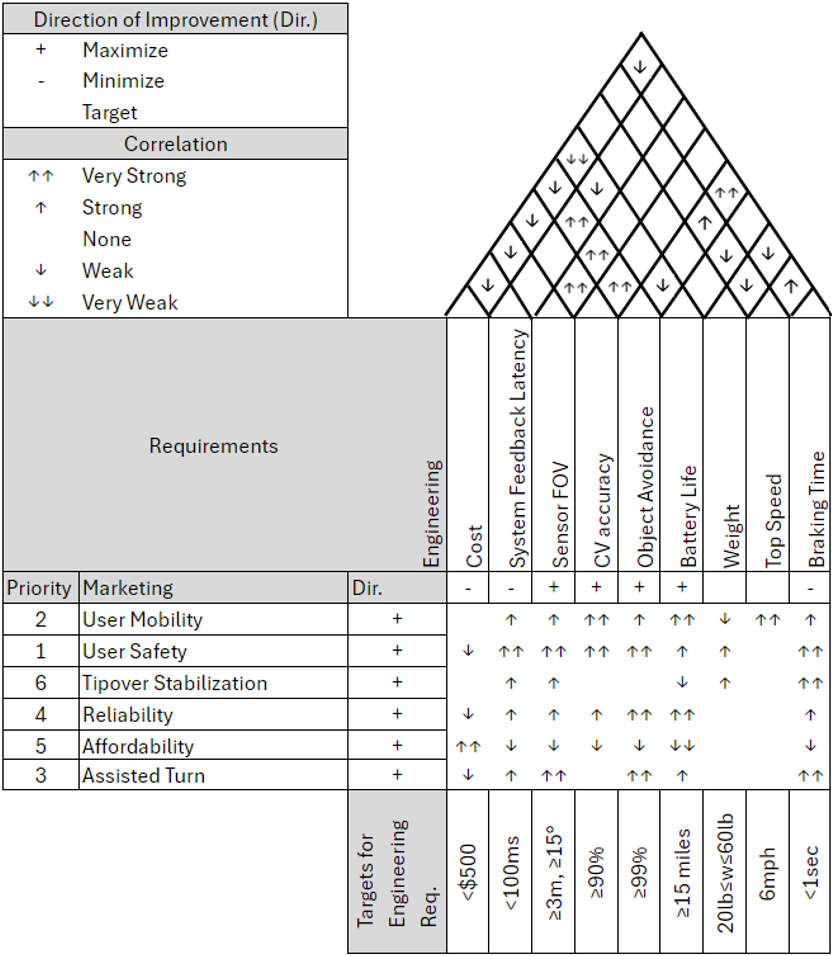
\includegraphics[width=\textwidth]{./Images/HoQ.png}
	\caption{\label{fig:HoQ}House of Quality}
\end{figure}

%\noindent Note that our house of quality diagram roof is diagonally placed. In essence, each diagonal axis is comparing its left neighbor to each other parameter it crosses as it traverses vertically. For instance, the topmost diagonal just under the roof line is comparing cost to system feedback latency, then to sensor FOV, and so on. The next diagonal is comparing system feedback latency to sensor FOV, CV accuracy and so on. \\

\noindent
Note that the engineering requirements from Figure \ref{fig:Standards} are encapsulated on the house of quality as cost, system feedback latency (end-to-end, sensing to user feedback), sensor FOV, CV accuracy, object avoidance (primarily refers to steering protocols), battery life, weight, top speed, and braking time. The ability to efficiently reconcile the marketing requirements with these engineering requirements will spell a great product after design is completed. 

	\subsection{Project Block Diagram}

\noindent As indicated by color and work breakdown delegation, the three subsystems of obstacle detection, identification, and avoidance are shown. The peripherals, depicted in the diagram by circles, are functionally sensors and feedback for user guidance. \\

\noindent The microcontroller unit is central to system integration. It will receive and transmit data from the peripherals while also communicating with the motor controller to steer and drive. In turn, the position determination algorithm, coupled with the speed and steering control, comprise the object avoidance function. Computer vision and image processing are also encompassed by this obstacle identification subsystem. \\

\noindent Headlights are an optional advanced requirement feature configured to turn on in lowlight environments. Finally, an implicit element of the diagram are the power inputs from the battery supply.\\

\noindent As seen below, each of the team members will be taking a lead role for different subsystems of the project. These roles were divided based on individual interests and skills, seeking to maximize overall productivity and effectiveness for the designs specified.

\noindent Tobiah, being an electrical engineering student with a focus in signal processing, will be covering the obstacle detection subsystem. This will involve research regarding the sensors and generating the range solution. The task at hand is then to give the walker vision of its surroundings without using cameras or any form of pre-planned pathing. FORWARD should be a reactive guidance system. \\

\noindent Morgan, being an EE interested in robotics and power, will be covering all subsystems under those categories. This includes the power supply as well as the more electromechanical components of the project such as the motors, headlights, and haptic feedback. The power supply will need to provide energy both to the MCU and to the different outputs. The MCU will then control these outputs, the headlights directly through the MCU and the motors for the wheels and haptic feedback using a motor controller. This will allow the system to functionally turn and avoid obstacles as well as vibrate to alert the user of obstacles. \\

\noindent As depicted by the blue shading, Matthew will be taking lead over most of the software related subsystems as well as the MCU. Since the camera will be primarily involved in transmitting video to the MCU for AI image processing – Matthew will be responsible for selecting the camera. The Audio Feedback Guidance will also involve heavy software support since it will be over Bluetooth, so this is also within Matthew’s scope. The MCU will drive everything, facilitating all communication through embedded programming and so it is also within Matthew’s scope.

\begin{figure}[H]
	\centering
	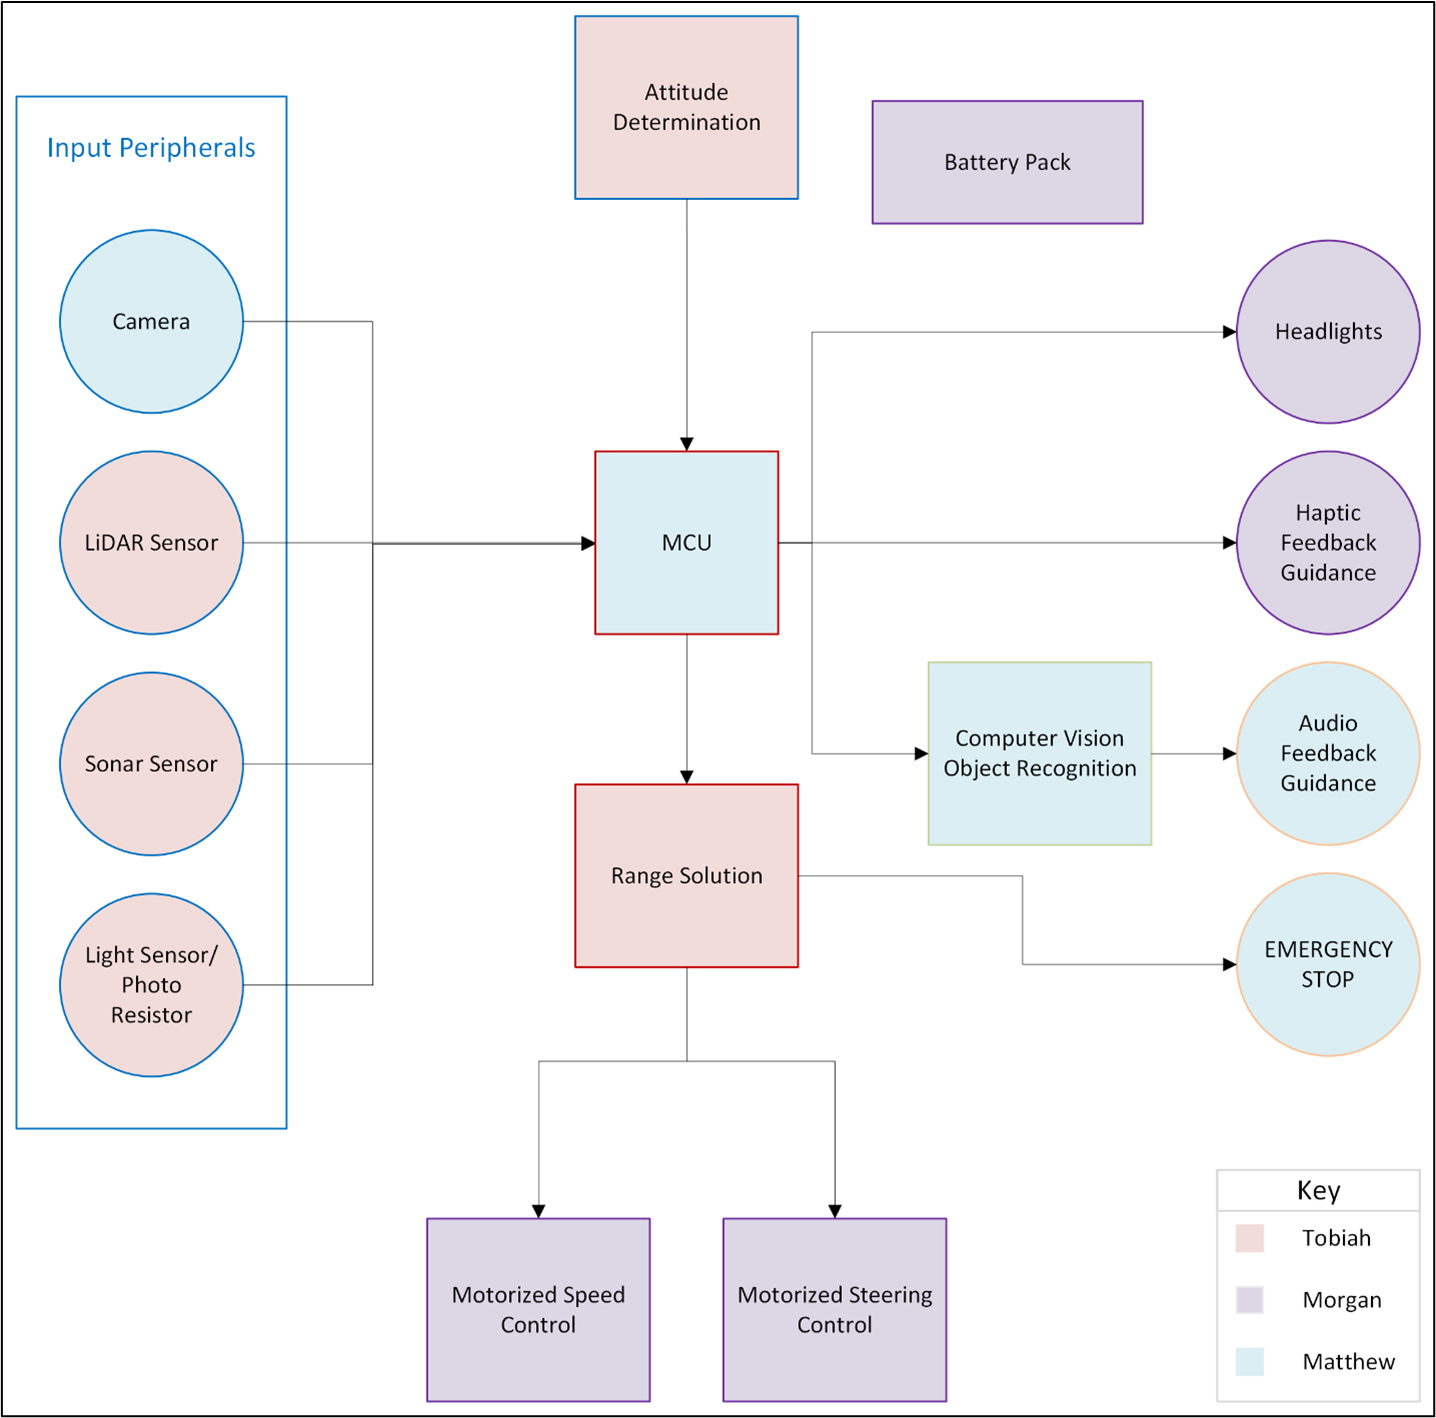
\includegraphics[width=0.95\textwidth]{./Images/AbstractSysBlk.png}
	\caption{\label{fig:AbstractSysBlk}System Block Diagram}
\end{figure}

	
	% 30 pages
	% due 09/10 - order parts ASAP!
	\newpage
	\section{Research}
	\subsection{Existing Products and Projects}
% how have other projects and products used similar strategies to FORWARD?

\noindent There have been numerous efforts made by researchers to develop smart walkers using the available technologies. Perhaps the seminal work in this growing field of research and development is \cite{PAMM}. This group was the first to propose a smart walker project with localization, mobility control, and object avoidance. In the following sections we seek to analyze these technologies and methods in a way that identifies which of such will be most desired for our specific system, taking into consideration many factors, some of which being: cost, attainability, integration complexity, and performance.

%% Toby research here
\subsubsection{Current Walker Sensing Applications}
\noindent In the smart walker prototype created in \cite{Mostofa}, nine HC-SR04 ultrasonic sensors are arrayed along the front of the walker. Seven face forward, while the remaining two point perpendicularly to the walker motion and opposite to each other. This setup provides a continuous reading of the walker's forward hemisphere with a detection range of 200cm. Our team asks the question, can obstacle detection and notification be achieved with a more discrete array of sensors stowed onto the walker frame? What is the operational FOV for ultrasonic sensors? Can the amount be reduced? How will the introduction of LiDAR and camera technology affect the ultrasonic approach?\\

\begin{figure}[h]
	\centering
	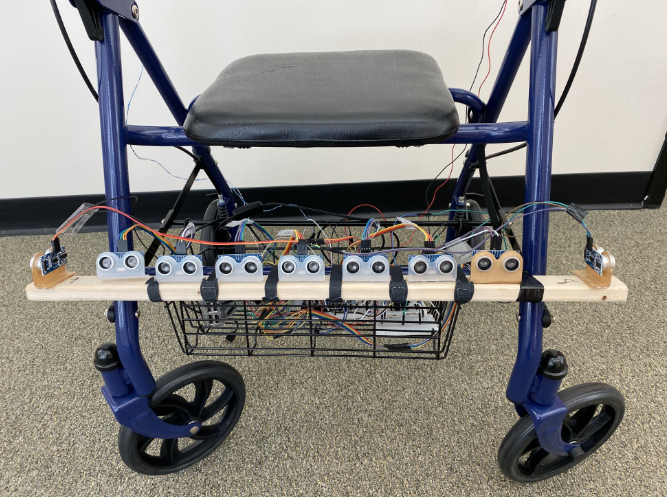
\includegraphics[width=0.5\textwidth]{./Images/mostafa9.png}
	\caption{\label{fig:mostafa9}"Rollator" with nine HC-SR04 sensors \cite{Mostofa}}
\end{figure}

\noindent Robotics are a popular use of LiDAR, often able to achieve feats such as autonomous delivery. However, many researchers have also introduced laser sensing methods and other waves near infrared in order to provide ranging data to mobile systems, which in our case is the walker. A senior design group at Michigan State University expanded on this \cite{mstate}.\\

\noindent In \cite{FallDetect}, the group implements one of FORWARD's stretch features with an unorthodox yet clever utilization of LiDAR and sensor fusion. In order to equip the walker with fall detection, both ultrasonic and laser sensors are installed near the footstep bay of the walker. They also add force sensors in the handlebars. The feedback provided by the sensing system is whether the user is walking uprightly. If the user began to fall, the laser sensors would reflect their feet moving out of view, and likely the force sensors would experience more pressure as the user reacted to a slip. \\

\noindent This walker does not employ GPS. We are not looking to track the location continuously. This technology has more of a place within the application of health monitoring and emergency alerts.\\


%% Matthew Research Here
\subsubsection{Existing Computer Vision/AI Image Processing Models}
 \underline{\textit{Ultralytics YOLO}} (You only look once) is an open source AI driven image processing model. The Ultralytics YOLO platform provides an AI Image processing Architecture that is malleable to the users demands, and for our case, would process the input image to detect if one of the five hazards is present, as well as provide a confidence rating for these predictions. To implement the object detection functionality to our specifications, minimal training, as well as coding must be performed. The benefits of this solution for our image classification system include zero cost and easy configurability which are both important aspects for our desired solution. The negatives include the needed man hours to train and implement this model for our purposes and time to run (anywhere from 0.1 seconds to 3 seconds). It also has a relatively high memory footprint (a few hundred MB). The time to predict along with the memory footprint could potentially exclude this from our options as we need to have classification under 1 second latency, ideally in the realm of a few hundred milliseconds and enough storage space for the model. \\
%https://www.freecodecamp.org/news/how-to-detect-objects-in-images-using-yolov8/#heading-how-to-get-started-with-yolov8 

\noindent \underline{\textit{FOMO}} (Faster objects, More objects) is a machine learning image processing algorithm that seeks to solve the problem of running high complexity algorithms (such as neural networks) on MCU's. In the documents referenced [HERE], the Arduino Nicla board is used to classify the objects in frame at a rate of 33 microseconds (30 SPS). The objects can be classified and processed through multiple methods, but all of which would be applicable to our purposes. This system also minimizes the memory usage by needing only 256 KB of memory to run and store these algorithms. On the FOMO website, they claim that this algorithm is compatible with many of the MCU's that we are considering for this project, some of which being an ESP32, Arduino Nicla, Raspberry Pi, and others. \\
%https://www.hackster.io/mjrobot/tinyml-made-easy-object-detection-with-nicla-vision-407ddd
%https://docs.edgeimpulse.com/docs/edge-impulse-studio/learning-blocks/object-detection/fomo-object-detection-for-constrained-devices

\noindent \underline{\textit{Spatial AI}} is the combination of both Visual AI and Depth AI, in tandem to identify objects for classification as well as identifying depth of objects for better guidance and classification. [Research the models that make this possible]\\
%https://learnopencv.com/object-detection-with-depth-measurement-with-oak-d/

\subsubsection{Existing Camera Technologies}
\noindent \underline{\textit{ESP 32 CAM Board}} is a ESP32 processor based camera module that can transmit video data at high resolutions, which can be processed by our CV/Image processing solution. The module also has WIFI connectivity that can connect to an MCU to wirelessly transmit the video stream. The module has a 32-bit CPU with a max clock frequency of 240 MHz and 520 KB of built-in SRAM with an external 4MB PSRAM. The board module also runs on FreeRTOS. The included camera, OV2640 camera, has a 2 MP resolution, up to 1600 x 1200 and interfaces the controller board over a 24 pin interface bus. A more advanced sister product to the OV2640 is the OV5640 camera. This camera has 5 MP resolution, up to 2592 x 1944. In order to achieve our stretch requirement of depth perception analysis for guidance and navigation, this camera could be advantageous.\\
%https://how2electronics.com/esp32-cam-based-object-detection-identification-with-opencv/
%https://how2electronics.com/getting-started-with-esp32-cam-board-video-streaming-over-wifi/

\noindent \underline{\textit{The Oak-D Lite}} camera is an AI robotics specific camera, capable of running AI models such as open CV. The camera is able to run on-board AI architectures to achieve object classification, edge detection, and feature tracking. This technology allow for high accuracy with object detection, and introduce the ability to implement edge detection as a means to depth perception, which can be used for routing in our GNC subsystem. The Oak-D Lite has a 13 MP RGB camera with auto-focus, as well a 60axis sensor using an accelerometer and gyroscope. It also uses USB2 and USB3 for power and communication, which is simple to interface to a RaspberryPI. The camera can run 4K at 30 FPS or 1080P at 60 FPS.\\


\subsubsection{Existing MCU Technologies}

\noindent 


%% Morgan Research Here
\subsubsection{Motor and Steering Applications} 


	\subsection{Relevant Technologies}
% compare the available technologies and propose how to apply them to our system

\subsubsection{Sensor Ranging}
% Toby - sensors, haptics
\noindent Ranging sensors are used to provide range information for a plethora of products today. They are popularly found in robotics, where they are able to provide awareness of the surroundings, vehicles, where they enable autonomous navigation, or for smart facility and home solutions, where they detect movement and are used to trigger various actions. FORWARD requires sensors to enable safe navigation and it is thus appropriate to examine the technologies available to determine which to utilize.\\

\noindent \underline{\textit{Time-of-Flight}} sensors are not suitable for FORWARD because of their narrow field of vision.\\

\noindent \underline{\textit{Global Positioning System}} One of the constraints in FORWARD is to navigate without GPS.\\

\noindent In this project, we utilize ultrasonic sensing as 1) mono and multistatic, 2) active, and 3) .\\

\noindent We deploy LiDAR in the context of this project as 1) oriented laterally, 2) topographic, and 3) . Typically, LiDAR has a. ALso consider reflectivity and ambient lighting\\

\noindent We also use IMU technology for the purpose of obtaining the acceleration and body rate readings of the walker.\\

\noindent Sensor fusion is  \\

% Matthew - MCU, computer vision, audio

% Morgan - Power supply, motors, motor shield, steering, braking
	\subsection{Strategic Components}
% this is pretty much all research about the components themselves, which is summed up with the spec comparison table in 3_5-partselect

\subsubsection{Ultrasonic Sensors} \label{sssec:tof}
\noindent The range solution according to \textbf{\textit{time-of-flight sensing}} is modeled by the simple equation, where $d$ is distance, $t$ is time to send and return an ultrasonic pulse, and $v$ which is the speed of sound (340m/s):
$$d = 1/2 \times t \times v$$

\noindent \underline{\textit{HC-SR04}} ECHO pin outputs the time, $t$, taken by the emitted sound pulse (TX) to return (RX). In practice, to continuously sense and report range, the microcontroller will repeatedly send 40kHz pulses to the sensor's TRIG pin, which are redirected by the transmitter as a beam. Using I2C, the microcontroller can read $t$ and perform the range calculation.\\

\noindent \underline{\textit{HRLV-MaxSonar MB1000}} This sensor features auto calibration, range filtering and many more output options: pulse width, analog voltage, ranging start/stop (real time), and serial output. The designers also claim that this higher quality sensor does not skew the range reading based on the target size as others do. To solve for range, either connect Pin 3 to an analog-to-digital converter and calculate:
$$d (mm) = bits_{\{0..1023\}} \times 5$$
Alternatively, Pin 4 gives options for real time range data based on its pull-up voltage. It can return a range on command by MCU or default to 2Hz filtered range data "based on recent ranges." Finally, Pin 5 is serial output in RS232 format, which sends in ASCII, the range in millimeters.\\

\noindent \underline{\textit{RCWL-1X0X}} sensors allow for the same solutions method as the HC-SR04 and MB1000. These models feature both UART and I2C serial outputs, in which the distance is read directly from the device using:\\
UART: $Distance = ((BYTE_H << 16) + (BYTE_M << 8) + BYTE_L) /1000$\\
I2C: $Distance = ((BYTE_H\&It; \&It; 16) + (BYTE_M\&It: \&It; 8)+BYTE_L) /1000$\\

\noindent \underline{\textit{H2KA150KA1CD00}} operates at the high frequency of 150kHz. Unfortunately, the datasheet does not reveal much more about solving the range than the need to use a rectangular wavwdrive signal and a burst of 10 pulses. This returns an analog voltage output of the range. At a directivity angle of 8+/-2 degrees and a short range viability, this is not an ideal option for FORWARD.\\

\subsubsection{LiDAR Sensors}
\noindent \underline{\textit{LiDAR Lite V3}}
1 Write 0x04 to register 0x00.
2 Read register 0x01. Repeat until bit 0 (LSB) goes low.
3 Read two bytes from 0x8f (High byte 0x0f then low byte 0x10) to obtain the 16-bit measured distance in centimeters \\

\noindent \underline{\textit{XT-S1}} allows for active continuous measurement of range by reading start address $0x00$. Its output is hexadecimal, which is easily converted to a decimal reading in millimeters.\\

\noindent \underline{\textit{TF Family}} LiDAR sensors allow continuous ranging and also read by command. Note these have a 20cm dead zone. The designers note the possibility of light shedding on two parts of a surface, at which the range reading could be any value inbetween. They advise avoiding this for reliability. In the greater FORWARD context, we can consider the lesser of the readings for safety, so this is not necessarily an issue.\\

\subsubsection{Inertial Measurement Units}
\noindent Because of the simplistic nature of the application of this technology in FORWARD, extensive research is not as necessary as with the range sensors. We consider two main options.\\

\noindent \underline{\textit{BN-0055}} is a 9-DOF (axis) IMU, meaning it contains a 3-axis accelerator, 3-axis gyroscope, and a 3-axis geomagnetic sensor. This device is said to run sensor fusion on-board to provide accurate attitude information. It runs on $2.4-3.6V$ and draws $0.4mA$ of current when on its low power mode. It can be used in 3-axis only modes, meaning you can isolate the accelerator, gyroscope or magnetometer.\\

\noindent \underline{\textit{MPU-6050}} is one of the most popular IMU devices. It is 6-DOF (no magnetometer), and runs a DMP (digital motion processor) for motion fusion algorithms. Essentially, it calibrates itself, and is said to reduce gyro drift by eliminating cross-axis alignment errors between the gyroscope and accelerator. It operates at $3.6mA$ with a supply of $2.4-3.5V$.\\

\subsubsection{Computer Vision/AI Image Processing Models}
\underline{\textit{Ultralytics YOLO}} (You only look once) is an open source AI driven image processing model. The Ultralytics YOLO platform provides an AI Image processing Architecture that is malleable to the users demands, and for our case, would process the input image to detect if one of the five hazards is present, as well as provide a confidence rating for these predictions. To implement the object detection functionality to our specifications, minimal training, as well as coding must be performed. The benefits of this solution for our image classification system include zero cost and easy configurability which are both important aspects for our desired solution. The negatives include the needed man hours to train and implement this model for our purposes and time to run (anywhere from 0.1 seconds to 3 seconds). It also has a relatively high memory footprint (a few hundred MB). The time to predict along with the memory footprint could potentially exclude this from our options as we need to have classification under 1 second latency, ideally in the realm of a few hundred milliseconds and enough storage space for the model. \\
%https://www.freecodecamp.org/news/how-to-detect-objects-in-images-using-yolov8/#heading-how-to-get-started-with-yolov8 

\noindent \underline{\textit{FOMO}} (Faster objects, More objects) is a machine learning image processing algorithm that seeks to solve the problem of running high complexity algorithms (such as neural networks) on MCU's. In the documents referenced [HERE], the Arduino Nicla board is used to classify the objects in frame at a rate of 33 microseconds (30 SPS). The objects can be classified and processed through multiple methods, but all of which would be applicable to our purposes. This system also minimizes the memory usage by needing only 256 KB of memory to run and store these algorithms. On the FOMO website, they claim that this algorithm is compatible with many of the MCU's that we are considering for this project, some of which being an ESP32, Arduino Nicla, Raspberry Pi, and others. \\
%https://www.hackster.io/mjrobot/tinyml-made-easy-object-detection-with-nicla-vision-407ddd
%https://docs.edgeimpulse.com/docs/edge-impulse-studio/learning-blocks/object-detection/fomo-object-detection-for-constrained-devices

\noindent \underline{\textit{Edge Impulse}} is a website that is free to use and will allow for you to train models and then generate code for specific target devices. The way it works is, you upload your images for object detection, label and frame the objects, and then train the model. After this, you can choose your target device (Edge Impulse supports RaspberyrPi, ESP32, Arduino, and more), and generate a zip file for a library of object detection code. This is a simple to use, low complexity option that supports all of our considered MCUs.\\
%https://edgeimpulse.com/
%https://www.youtube.com/watch?v=bZIKVaD3dRk\

\subsubsection{Camera Technologies}
\label{sec:cam_tech}
\noindent \underline{\textit{ESP 32 CAM Board}} is a ESP32 processor based camera module that can transmit video data at high resolutions, which can be processed by our CV/Image processing solution. The module also has WIFI connectivity that can connect to an MCU to wirelessly transmit the video stream. The module has a 32-bit CPU with a max clock frequency of 240 MHz and 520 KB of built-in SRAM with an external 4MB PSRAM. The board module also runs on FreeRTOS. The included camera, OV2640 camera, has a 2 MP resolution, up to 1600 x 1200 and interfaces the controller board over a 24 pin interface bus. A more advanced sister product to the OV2640 is the OV5640 camera. This camera has 5 MP resolution, up to 2592 x 1944. In order to achieve our stretch requirement of depth perception analysis for guidance and navigation, this camera could be advantageous.\\

\noindent \underline{\textit{Oak-D Lite}} is an AI robotics specific camera, capable of running AI models such as open CV. The camera is able to run on-board AI architectures to achieve object classification, edge detection, and feature tracking. This technology allow for high accuracy with object detection, and introduce the ability to implement edge detection as a means to depth perception, which can be used for routing in our GNC subsystem. The Oak-D Lite has a 13 MP RGB camera with auto-focus, as well a 60axis sensor using an accelerometer and gyroscope. It also uses USB2 and USB3 for power and communication, which is simple to interface to a RaspberryPI. The camera can run 4K at 30 FPS or 1080P at 60 FPS.\\

\noindent \underline{\textit{Realtek AMB82-Mini IoT AI Camera}} is a lower cost option (\$25) to incorporate an AI object detection system within the camera and board. The specifications of the device are as follows: The MCU is an ARMv8M running up to 500 MHz, accompanied by an NPU with an Intelligent Engine capable of 0.4 TOPS. It features 128 MB of internal DDR2 memory. Connectivity options include dual-band Wi-Fi and Bluetooth 5.1.The audio code supports ADC/DAC/I2S, and the ISP/Video functionality includes both 1080p and 720p at 30FPS. The camera module is a JXF37 full HD CMOS image sensor with a resolution of 1920 x 1080 and a wide-view-angle FOV of 130°. The interface includes 1 microphone, 2 Micro USB B ports, 1 MicroSD card slot, and support for 3 UARTs, 2 SPIs, 1 I2C, 8 PWMs, 2 GDMAs, and a maximum of 23 GPIOs. This solution would free up processing power on our MCU which could be of great value given the high workload placed on our MCU including sensor fusion, motor controlling, image processing, and other needed functionalities. Also, due to the high memory capacity (128 MB DDR2), we could implement a higher quality detection model.\\


\subsubsection{MCU Technologies}
\label{sec:mcu_tech}
\noindent The Embedded Processor/MCU for the project will be the "brains" of the system. It will bring together every other subsystem cohesively and run all necessary computations, while needing to maintain a minimal footprint in aspects such as power and physical size. We must also consider the cost effectiveness. It will also need I2C communication buses to interface the Sonar and LiDAR Sensors, Bluetooth to communicate with the audio feedback device, WiFi to communicate with the Camera, and UART/SPI/I2C to interface with the motor drivers/controllers. Given all of these needs and constraints, we will be looking into the current state of MCU products. \\

\noindent \underline{\textit{The ESP32 MCU}} is a small but powerful microcontroller with many features. These features include UART, SPI, and I2C communications, 4 MB - 8 MB of flash, with some PSRAM options. These boards also have WIFI and Bluetooth connectivity. The ESP32 series of MCU's range anywhere from \$9 to \$12. The current existing boards are ESP32-DevKitC-32E, ESP32-DevKitC-32UE, ESP32-DevKitCVE, ESP32-DevKitCVIE, and ESP32-DevKitCS1. The main difference between these boards are size and types of memory (4 MB - 8 MB and PSRAM/FLASH) along with antenna type (IPEX vs PCB). The ESP32 family also has a variety of products, such as camera modules, motor controllers, and others. The ESP32 is also easy to program as it is compatible with the Arduino IDE. \newline

\noindent The final consideration for the ESP-32-WROOM DevKitC is which of the variation would best fit our purposes, the standard, U, or D series. The D contains a differen PCB design relative to the standard which improves RF performance. The U is optimized for wider range WiFi capabilities due to an external IPEX antenna. The cost is slightly different coming in at \$6.67, \$6.67, and \$7.50 respectively. The D is the best fit for our purposes given we don't need wide range WiFi since the system is within a cubic meter in size, but the RF performance improvement of the D would be helpful given we will be transmitting our camera data over WiFi. \\
%https://www.espressif.com/en/products/devkits/esp32-devkitc

\noindent \underline{\textit{The RaspberryPI 4 model B}} is a small computer with a 64-bit quad core processor running at 1.5GHz. The RaspberryPi has both dual-band 2.4GHz and 5GHz wireless LAN and Bluetooth 5.0/BLE. The Pi also has Ethernet capabilities along with a 40 pin GPIO header. It uses the Broadcom BCM2711 processor chip and comes with memory options of 1GB, 2GB, 4GB or 8GB LPDDR4-3200 SDRAM, as well as having a micro-SD slot for additional memory capabilities. The board also features many I/O ports, such as 2 USB 3.0 ports, 2 USB 2.0 ports, 2 HDMI ports, and a 2-lane MIPI CSI camera port. The board ranges from \$30 to \$50 and can be purchased online. \\
%https://www.pishop.us/product/raspberry-pi-4-model-b-2gb/?src=raspberrypi

\noindent \underline{\textit{The Jetson Nano}} is a complex, high powered MCU designed for AI/ML applications. It is an NVIDIA product with a 128-core NVIDIA Maxwell™ GPU and a quad-core Arm® A57 CPU. It comes with 4 GB of 64-bit LPDDR4 memory and supports MicroSD storage. For power, it supports both 5 V, 4 A DC power and 5 V, 2 A via Micro-USB. In terms of connectivity, it offers a USB 3.0 Type-A port, a USB 2.0 Micro-B port, an HDMI/DisplayPort output, and Gigabit Ethernet. The board also includes various general-purpose input/output (GPIO) options, along with interfaces for I2C, I2S, SPI, UART, and a MIPI-CSI camera connector. These features make the Jetson Nano a robust solution for real-time processing tasks needed for guiding and navigating. This board is designed for running AI/ML applications. The MCU can cost anywhere from \$250 to \$500 depending on the model and specifications. \\

	\subsection{Possible Architectures and Related Diagrams}

\subsubsection{Proposed Sensor FOV Topology}
\noindent A ranging apparatus comprised of four ultrasonic sensors, one central LiDAR sensor, and optionally, a camera with spatial AI, should provide ample ability to FORWARD's object detection feature. Two wide FOV ultrasonic sensors face forward: one on each walker leg. Two face sideways, also mounted on the bottom half of the legs. The LiDAR sensor is mounted centrally so its beam detects straight-on obstacles. The camera is also mounted centrally. Finally, we angle these downward to allow for detection of obstacles present at the knee down height level. Additionally, a zero energy return from the ultrasonics or LiDAR could constitute a drop-off or ledge or divot. This will be elaborated upon in obstacle classification and identification.\\

\begin{figure}[H]
	\centering
	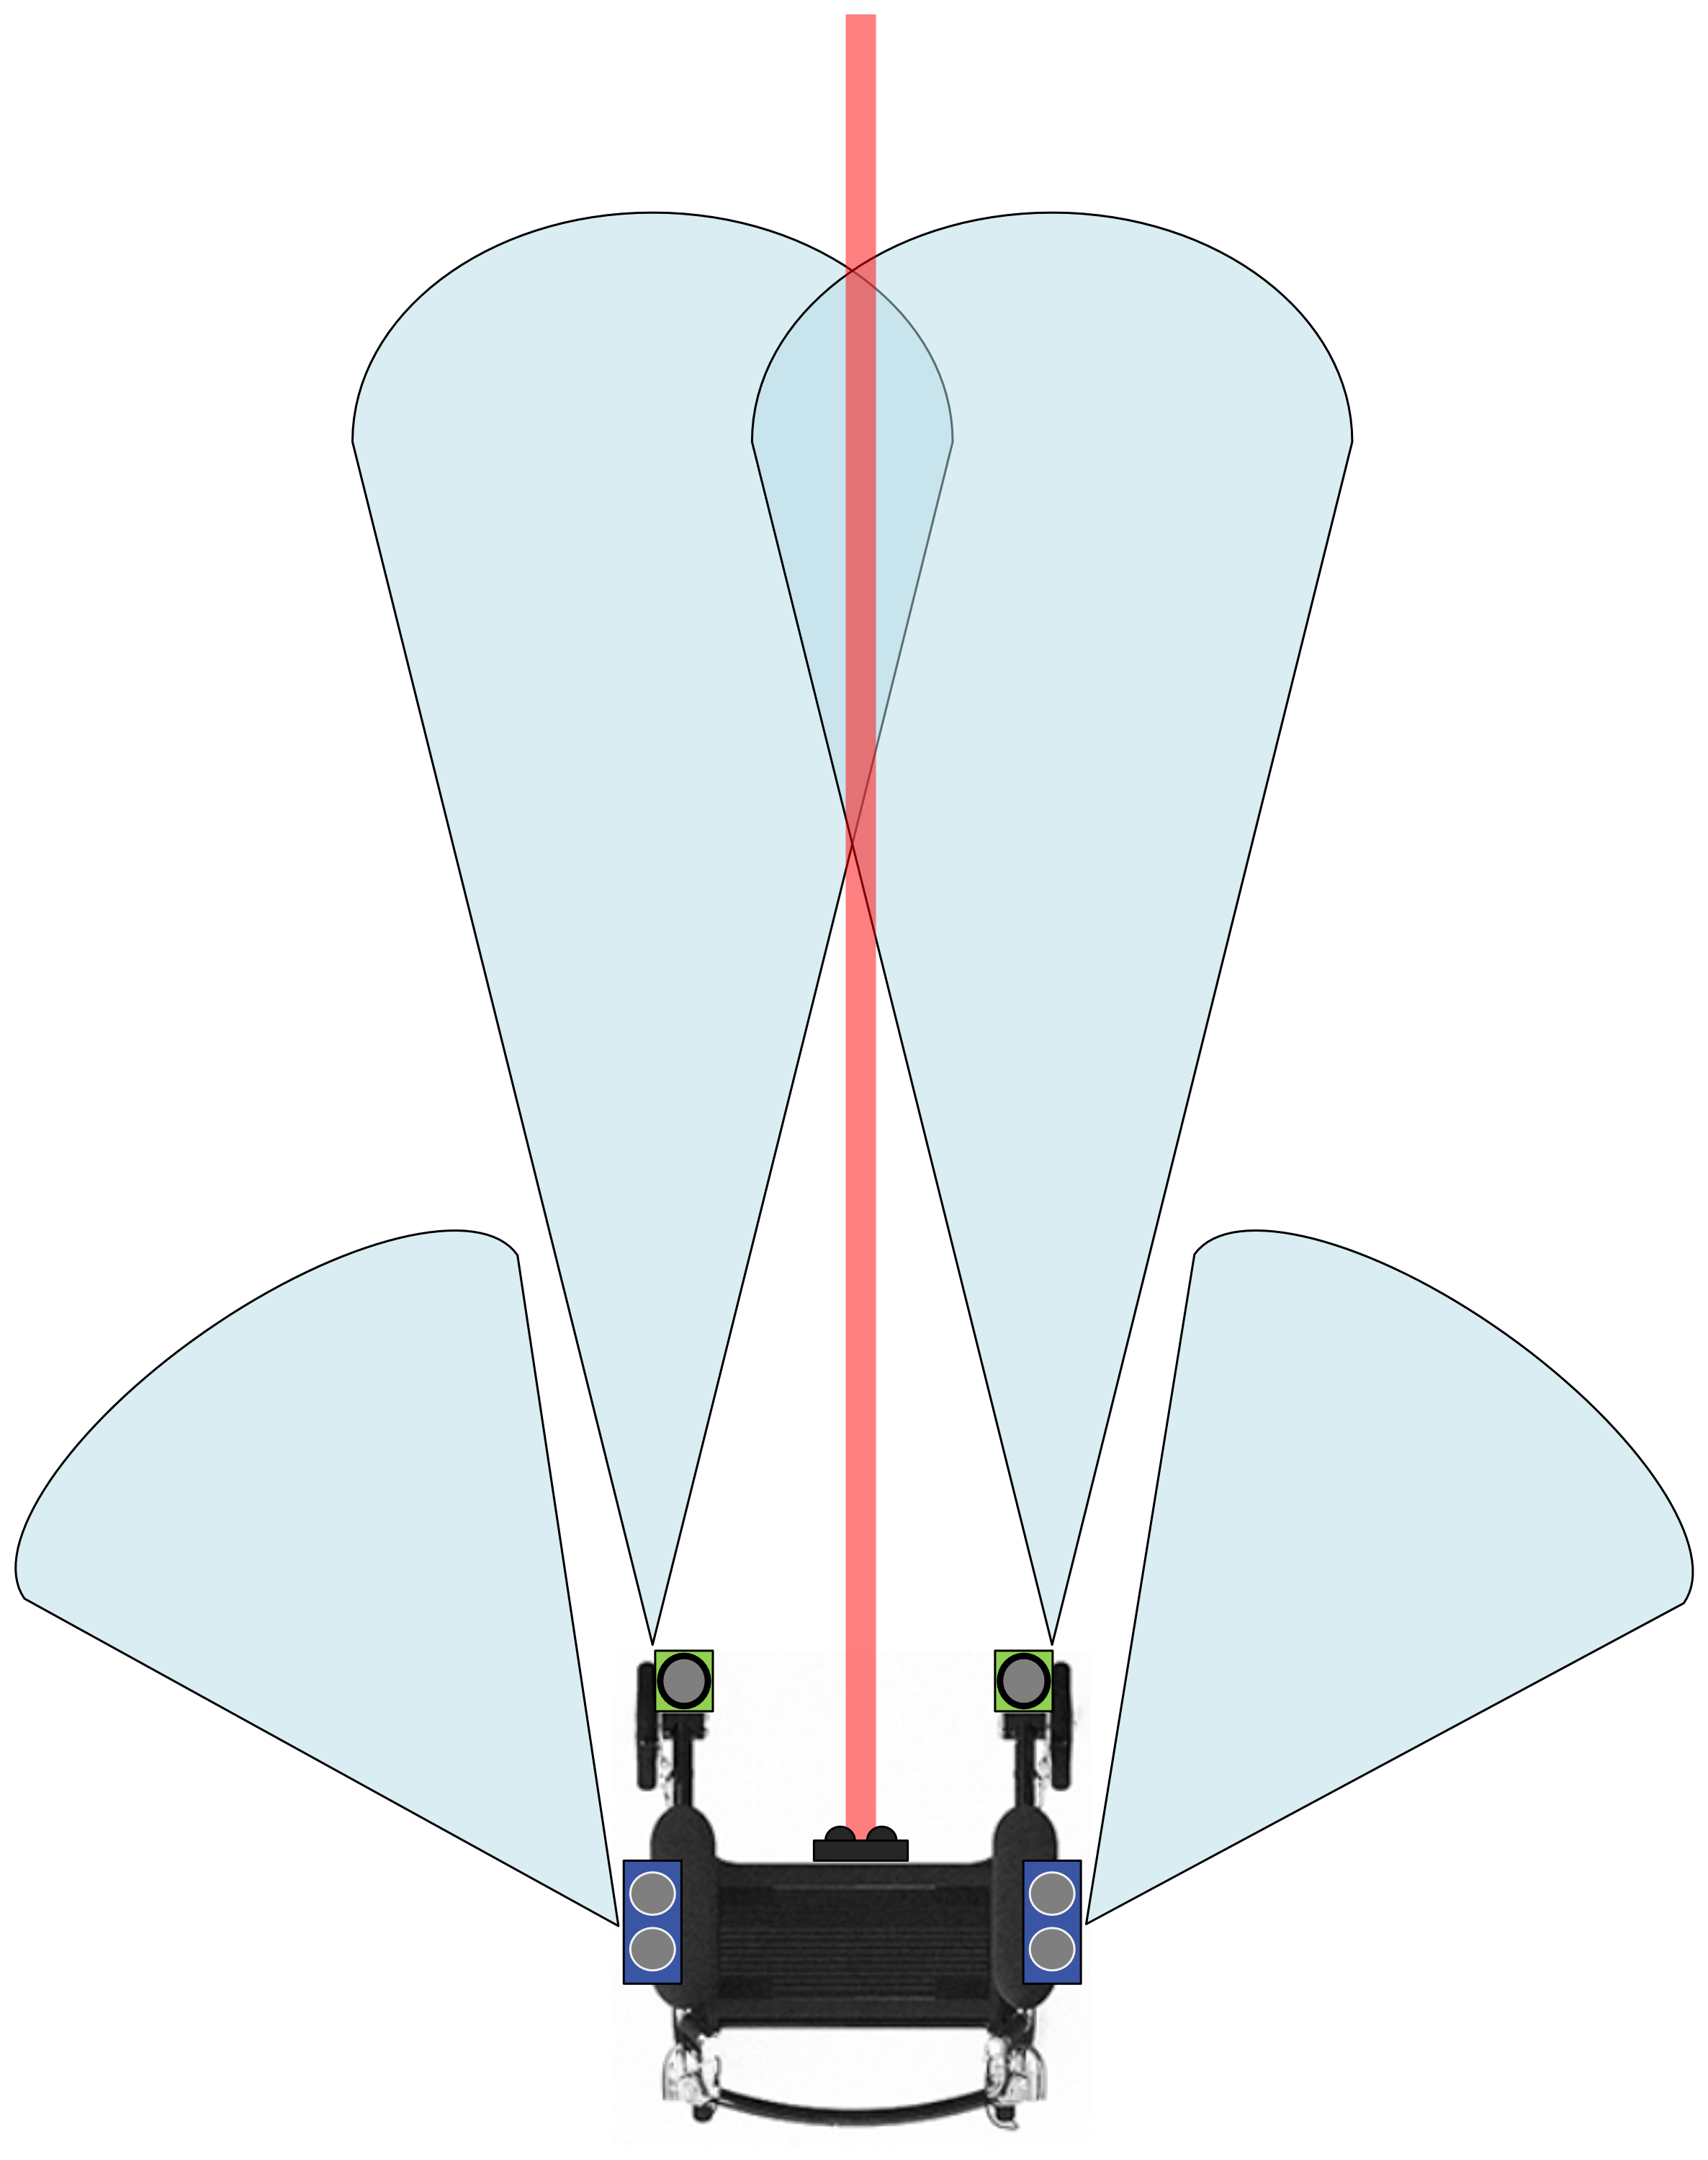
\includegraphics[angle=90,width=0.75\textwidth]{./Images/propose-sensorFOV.png}
	\caption{\label{fig:proposedsensorFOV}Proposed Sensor FOV (Range NOT to scale)}
\end{figure}

\noindent As mentioned in 2.2, the object detection data must work hand-in-hand with the identification and avoidance schemes. With identification, the range data is combined with any potential depth perception data generated by the camera. The closer the walker gets to the obstacle, the more urgently the system can respond. With avoidance, motor commands should be generated proportionately to the severity of the obstacle range-to-walker frame. Determining these specific plans of action is elaborated in later sections.\\

%\begin{figure}[h]
%	\centering
%	\includegraphics[width=0.7\textwidth]{./Images/FOVapparatus.png}
%	\caption{\label{fig:proposedFOVapparatus}Proposed Sensor Ranging Apparatus}
%\end{figure}

\subsubsection{Euler Angles}
\noindent Euler angles are one of our data streams that will inform FORWARD's guidance commands. We define a body reference frame whose center is the center of gravity of the rollator (with chassis and power supply mounted already). From there, we can monitor the \textit{attitude} $[\psi, \theta, \phi]$, or orientation, of the body frame, as represented by angles measured from the three major axes. The positive x-axis is defined as orthogonal to the front face of the rollator - in other words, forward looking-aft. Then, a positive rotation around this axis is defined as clockwise, or to the right, and results in a positive roll Euler angle, $\psi$. Next, we define the positive y-axis as perpendicular to the x-axis, using the right hand rule convention. A rotation about this axis is defined as positively clockwise, resulting in a positive pitch Euler angle, $\theta$. Finally, the positive z-axis is orthogonal to the xy-plane, and a positive rotation is rightwards. This results in a positive yaw Euler angle measurement $\phi$. We could theoretically define new reference frames, and perform coordinate transformations into those frames in order to gain new insight into the rollator attitude, but that is not necessary for the scope of this senior design project. We will simply monitor these angles to ensure stability, and aid the guidance of the user.\\

\subsubsection{Velocity and Position Solution}
\noindent With the addition of the IMU as indicated in section 3.3, FORWARD is able to resolve its relative velocity and position based on a starting point by twice integrating the accelerometer data output. By tracking these updates, FORWARD can be more self-aware of its current traveling state. Not only is the IMU useful for tilt detection (identifying incline and decline), but it can also be used to verify and validate the range data output by the LiDAR and sonar sensors. For example, the software can have some condition where, if the range decreases under a predetermined threshold of danger, then the IMU data can reset and begin tracking position and velocity, with that initial point as the origin of the reference frame. This can allow for very precise geometric abstracted data visualization of the free space ahead and the trajectory of the walker.\\

\subsubsection{Kalman Filter}
\noindent As part of the project stretch requirement for depth perception using an upgraded camera, implementation of a typical sensor fusion algorithm will help to predict the walker's trajectory and provide counteractive insight to the guidance system. Implementation of a Kalman filter estimator would not be beneficial for the fusion of the LiDAR and Sonar data, because the delta between these should be small, and thus, would not provide any helpful insight to FORWARD. However, if obtaining a second range solution from AI depth perception, this data could be fused to choose how much credence is given to either the standard range solution or the computer vision. Essentially, this functionality would be able to minimize measurement noise originating from the information loss of the sensors, and to maximize the overall precision of obstacle avoidance. \cite{kalman} \\

\noindent A Kalman Filter generates an estimation based on two measurements (that are likely noisy or deemed untrustworthy) by the following iterative algorithm:
\begin{enumerate}
	\item Initialize the state estimate and error covariance.
	\item Predict the next state and covariance based on previous states, covariance between successive measurements, and process noise (amount of credence given to either measurement).
	\item Update the measurement based on the Kalman gain.
\end{enumerate}

\subsubsection{Quaternions}
\noindent The BNO055 inertial measurement unit has a distinct advantage that involves a particularly interesting mathematical formulation. It is able to output quaternion data. Quaternions are a complex mathematical formulation which can be used as a replacement of sorts to \textit{Euler Angles}, mainly addressing the gimbal lock issue of Euler Angles, which occurs when two torus of rotation align and thus reduce the degrees-of-freedom. Quaternions generally are able to all for a smoother representation of rotations, using four dimensions (three imaginary) to transcend the three. \cite{quat} FORWARD will likely not make use of these, but they are quintessential in the field of guidance, navigation, and control, and thus warrant a mention in this study. See the fundamental representation:\\
$$i^2+j^2+k^2=ijk=-1$$

% matthew
\subsubsection{System Data Network}
\noindent The proposed system network for data transmission can be seen pictured below. The ESP32 MCU is the main controller for our system, bringing together the sensor data and the object detection data for the guidance and navigation aspect of FORWARD. The peripheral sensors: IMU, LiDAR, and Sonar are connected to the ESP32 through GPIO and I2C, in which data is transmitted continually. The ESP32 also hosts a wireless network in which the Ameba 82 camera module connects and transmits the object detection data through UDP sockets over WiFi. \\

\noindent The Ameba 82 also plays a crucial role in the networking of our system. It links the object detection data to the ESP32 and the user. As stated above, it transmits the calculated object data to the ESP32, but also transmits the audio of the objects name over Bluetooth to the AfterShokz, which will be to the end user. \\

\begin{figure}[H]
	\centering
	\fbox{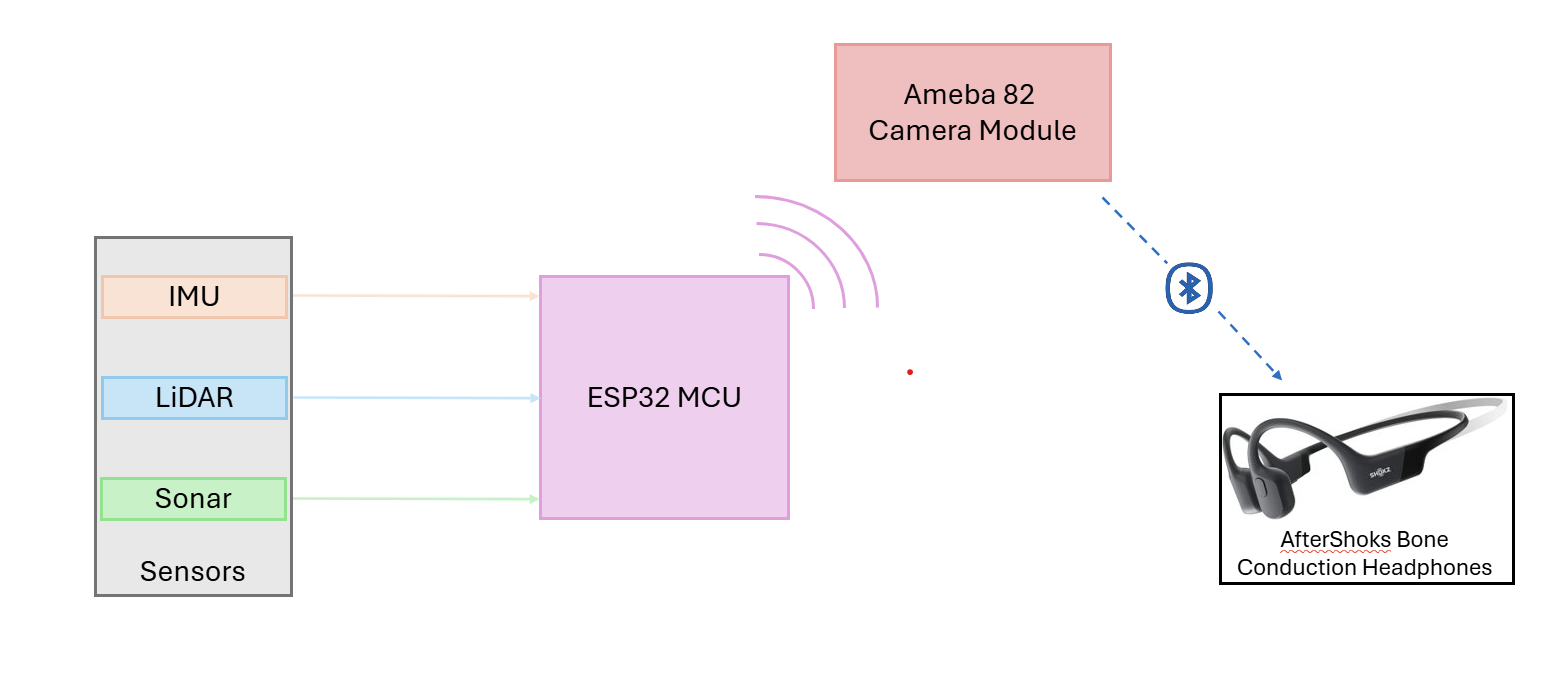
\includegraphics[width=1.0\textwidth]{./Images/System_Network_Arch.png}}
	\caption{\label{fig:System_Network_Arch}System Data Network Architecture}
\end{figure}


% morgan
\subsubsection{Typical steering motor control wiring}


	\subsection{Part Selection}
\noindent For \textbf{obstacle detection}, the final selections are:
\begin{enumerate}
	\item 2x HC-SR04 Multistatic Ultrasonic Sensors for lateral-facing detection.
	\item 2x RCWL-1005 Monostatic Ultrasonic Sensors for front-facing detection.
	\item The TFLuna LiDAR sensor, for its precision and accuracy. Front-facing. It has easy I2C configuration and a great price point, making it a viable option.
	\item The BNO-055 Inertial Measurement Unit because of its advantages like quaternion output and affordability, which greatly enhance FORWARD stability.
\end{enumerate}

\noindent For \textbf{obstacle identification}, the final selections are:
\begin{enumerate}
	\item The ESP32 MCU for affordability and diverse I/O ports. 
	\item The Realtek AMB82-Mini IoT AI Camera for high performance, cost-effectiveness, high image quality.
	\begin{enumerate}
		\item A stretch requirement of our project is to implement a depth perception capability with our system. Due to the sensor fusion solution that we are taking we have decided that we no longer need a super high-quality camera to obtain the depth data.
	\end{enumerate}
	\item The YOLO model family for memory size flexibility and user-friendly libraries for simple integration.
	\item The YouthWhisper Bone Conduction headphones for affordability and battery life.
\end{enumerate}


\noindent For \textbf{obstacle avoidance}, the final selections are:
\begin{table}[H]
	\centering
	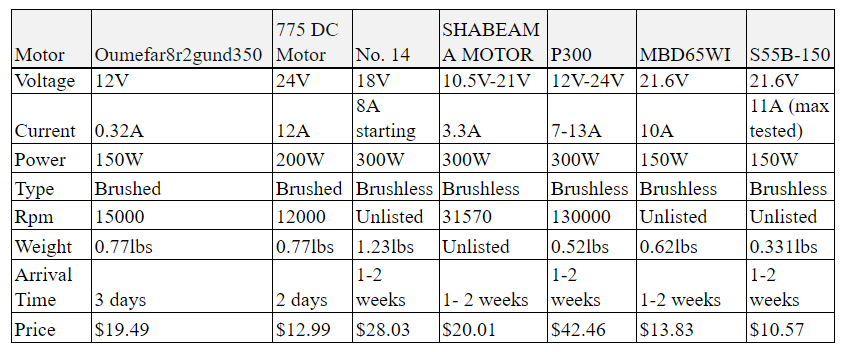
\includegraphics[width=1\textwidth]{./Images/drive_motors.png}
	\caption{\label{fig:drive_motors}Drive Motor Specifications}
\end{table}


\noindent When deciding on what DC motors that we wanted to use, our main concerns were power, current rating, motor type, and price. It was calculated that in order to meet the speed requirements, we needed a total of 300W or 150W per motor. All of the motors investigated thus are at least 150W. It was also preferable to use brushless DC motors, as they are higher in quality (longevity, efficiency, low noise) than brushed DC motors and are more widely compatible with motor drivers. To decide between the brushless DC motors, we mostly looked at price and found the most cost-effective motors, while also keeping in mind the current rating so that we can purchase motor drivers with a large enough current rating to supply the motors. Thus, we decided to use the S55B-150 DC motors. \cite{yzl1} \cite{Citphto} \cite{AliExpress1} \cite{AliExpress2} \cite{AliExpress3} \cite{PrecisionMicrodrives} \cite {AliExpress8}\\

\begin{table}[H]
	\centering
	\setlength{\tabcolsep}{5pt} % Restore default column padding
	\renewcommand{\arraystretch}{1.75} % Restore default row height
	\scalebox{0.85}{ % Scale down the entire table by 75%
		\begin{NiceTabular}{|l|c|c|c|}[hvlines,colortbl-like]
			\CodeBefore
			\rowcolor{gray!15}{1}
			\Body
			\textbf{Specification} & \textbf{B0B4SK8M1C \cite{DIANN}} & \textbf{A19090500ux0371 \cite{uxcell}} & \textbf{Vibration Motor \cite{eBayDC}} \\ 
			\hline 
			Voltage & 1.5-3.7V & 4.5-12V & 3-5V \\ 
			\hline 
			Current & 85mA & 250mA & 15mA \\ 
			\hline 
			Type & DC & DC & DC \\ 
			\hline 
			Arrival Time & 4 days & 4 days & 1-3 weeks \\ 
			\hline 
			Price (Qty) & \$5.99 (10) & \$10.99 (2) & \$9.21 (2) \\ 
		\end{NiceTabular}
	}
	\caption{\label{fig:vibrationMotorSpecifications}Vibration Motor Specifications}
\end{table}

\noindent Haptic motors are small DC motors that are used for vibration feedback in the handlebars of the walker. Because they are only used for the purpose of vibration, these motors are very small and do not draw much current. Our main concern with deciding which haptic motors to use is the voltage rating and price. In order to be compatible with most motor drivers, the motors should be able to be operated at both 5V and 3V. Although not the most cost-effective, we chose the "Vibration Motor" as it has the largest compatibility with motor drivers.\\

\begin{table}[H]
	\centering
	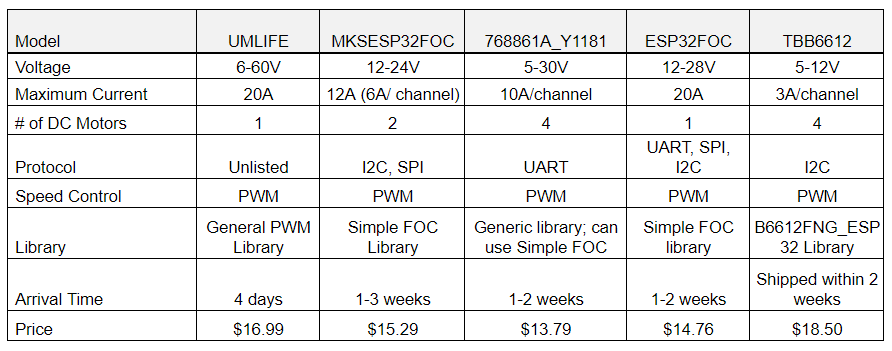
\includegraphics[width=1\textwidth]{./Images/motor_controller_table2.png}
	\caption{\label{fig:motor_controller}Motor Controller Specifications}
\end{table}

\noindent After comparing multiple factors, we ultimately chose the 768861A\_Y1181 motor controller. This is because our main concern was supplying current to the motors and operating all 4 motors from the same controller. The motors that we chose to drive the wheels draw up to 11A of current, which the 768861A\_Y1181 would be able to handle, although it is rated for 10A, upon examining the data sheet. This motor controller also provides a wide voltage range of 5-30V, which is able to provide the correct voltage for both the wheel-driving motors and the haptic motors. The 768861A\_Y1181 also happens to be the most cost-effective of the motor controllers. \cite{UMLIFE} \cite{AliExpress5} \cite{Makerbase} \cite{AliExpress7} \cite{CircuitBasics} \cite{Espressif1} \cite{AliExpress4} \cite{Burgess} \cite{RandomNerd} \cite{Espressif2} \cite{SimpleFOC} \cite{SimpleFOC2} \cite{Peza}\\


\begin{table}[H]
	\centering
	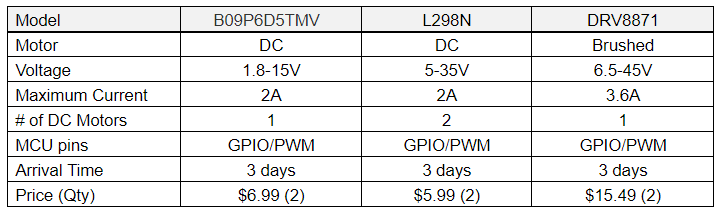
\includegraphics[width=1\textwidth]{./Images/haptic_driver_table_2.png}
	\caption{\label{fig:haptic_driver}Haptic Motor Driver Specifications}
\end{table}

\noindent This table compares the different motor drivers available for use with haptic motors.  decided to use the L298N motor driver as this solution is simply the most cost-effective. All of the haptic motor driver options available have similar ratings in voltage and current. We were also able to find more documentation for the L298N \cite{BOJACK} \cite{BEEYDC} \cite{HiLetgo}.\\

\begin{table}[H]
	\centering
	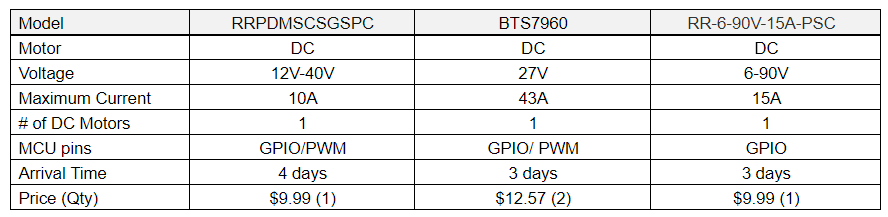
\includegraphics[width=1\textwidth]{./Images/wheel_driver_table.png}
	\caption{\label{fig:wheel_driver}Wheel Motor Driver Specifications}
\end{table}

\noindent Comparing options, we decided upon using the BTS7960 motor driver. The BTS7960 is able to supply more than enough current to the DC motors driving the wheels. This option is also the most cost-effective as the price includes two motor drivers to be able to drive both motors \cite{RioRand} \cite{Gikfun} \cite{Hobbywing}.\\

\begin{table}[H]
	\centering
	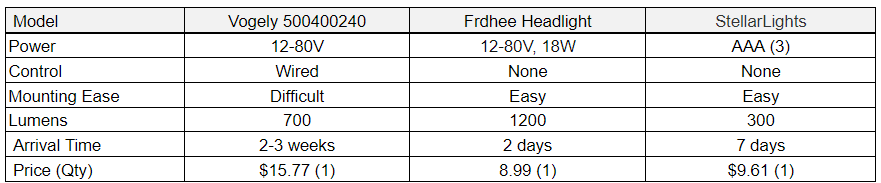
\includegraphics[width=1\textwidth]{./Images/headlight_table.png}
	\caption{\label{fig:headlights}Comparison of Headlight Options}
\end{table}

\noindent Comparing these different headlights that were originally intended for bicycles and motorcycles, we decided to use the Vogely ‎500400240. This is because these are the only headlights of these options that are able to be controlled digitally. Headlights are only necessary in dark environments, so we must connect the headlights to a light sensor. \cite{vogely2024} \cite{frdhee2024} \cite{stellarlights2024}\\

\begin{table}[H]
	\centering
	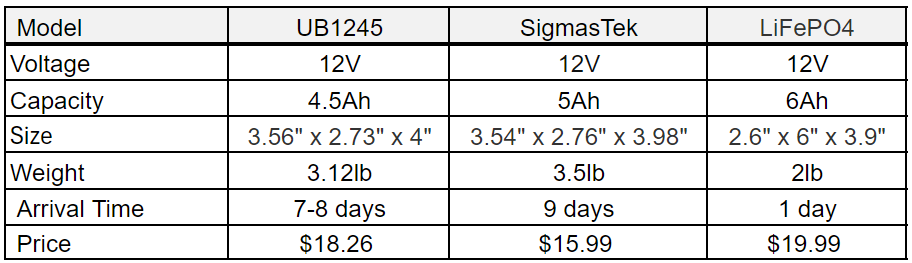
\includegraphics[width=1\textwidth]{./Images/battery_table.png}
	\caption{\label{fig:batteries}Comparison of Battery Options}
\end{table}

\noindent Comparing these different options for batteries, we decided upon using the SigmasTek battery. We evaluated 12V batteries since we ultimately decided on implementing 12V motors and these are our highest-voltage components. Comparing prices and capacity, we found that the SigmasTek battery was preferred because it provides the lowest cost for the needed battery capacity. \cite{liftmaster2024} \cite{lifepo42024}\\
	
	% 9 pages
	\newpage
	\section{Requirements, Standards, and Constraints}
	% intro paragraph
\noindent Chapter 4 discusses the related standards and constraints for both hardware and software used by FORWARD during development and realization. The main consideration for standards is given to connections, medical rollators, and IEEE guidelines on Bluetooth, wireless networks, sensors, motors, and serial communications. In addition, we examine constraints through the lenses of economic, environmental, social, political, ethical, health, and safety.

\subsection{Related Standards}
\noindent FORWARD must comply with all IEEE-related standards relating to sensors, motors, computer vision, and image processing. Taking a brief look at the specifics, none are immediately seen as hindrances to the proceedings of FORWARD’s research. Should an issue arise with IEEE-related standards later in the project, future documentation will indicate that. \\

\noindent IEEE also includes some standards relating to the testing of DC motors (IEEE 113-1985 \cite{ieee113277}). Although we cannot access this standard as it must be purchased, it mentions that there are standards for testing the ripple operations of DC motors as well as their use with rectifier power supplies. This is not a specification that correlates to our design, however, because we are not designing the DC motors themselves. We are simply using motors that have already been designed, tested, and evaluated.\\

\noindent IEEE also has a guide that is provided that gives insight to selecting the correct "valve-regulated lead acid batteries for stationary applications" \cite{ieee11893242}. This would be useful to ponder different factors in selecting the correct power supply. However, again, we are unable to access this document as purchasing is required. Although this document would be helpful, it is not necessary.\\

\noindent The ADA (American Disabilities Act) also has stipulations for environments to make accommodations for these assistive vehicles including walkers and electric wheelchairs. However, none of these should affect our design process, given that our product is safe to operate around other people and in busy environments.\\

\subsubsection{PCB Standards}
\noindent Some standards that may be relevant, however, include the IPC standards for PCB design \cite{ipc2221}. IPC is a trade association that seeks to ensure high-quality products by providing standards for electronics design and manufacturing. The standard IPC-2221 provides specifications for PCB traces and component spacing on the board. We would like to implement at least some of these of these standards so that our PCB can high-quality and reduce the probability of errors in our design. \\ 

\noindent Some of the primary implications of this IPC-2221 standard are the clearance between components on the PCB and the thickness of traces. Different components require different clearances between them; for example, a minimum clearance of 75mm is required between uncoated conductors and other components. The dimensions of the traces on the PCB are also a necessary consideration as current passing through a wire creates heat and may burn out the trace. Thus the thickness of the PCB trace is dependent on the surrounding temperature, width of the trace, maximum rated current, and constants. Below the formula is given \cite{ipc2221}. \\

\noindent \[A = I / ({k \times \Delta T ^ {0.44}}) ^ {1/0.725}\]

\noindent Another implication of the IPC-2221 standard is design considerations for the material of the PCB. A circuit board should have insulating material (at least one layer) between components so that there is electrical isolation and nothing is shorted. It is essential that this material is a good insulator, particularly if the PCB is meant to withstand higher voltages. We plan to use motor drivers within our design for potentially high voltage motors. Thus, we especially need to consider selecting materials that follow the insulation test specifications established by IPC-2221. These are materials with a high CTI (critical tracking index) rating, which have a larger breakdown voltage.\\

%\noindent Another standard that relates to PCB design is 

\subsubsection{Soldering Standards}
\noindent Another IPC standard that we thought to be relevant also relates to the fabrication of the prototype connecting with the PCB in terms of soldering. Due to economic constraints, we are unable to purchase the set of standards defined by IPC J-STD-001J, however, we have access to the table of contents of these soldering standards. This document encompasses over 70 pages of standards related to soldering, some of which include lead forming, unintentional bending, thermal protection, soldering to terminals, wire routing, flux application, and high frequency/voltage applications \cite{ipc_standard}. These are just a handful of topics covered, many of which have some relevance to our project. Although we are incapable of viewing the standards themselves, they still give us an appropriate baseline of applicable factors to consider. From there, we can further research any topics that we believe require attention.\\

\noindent IEC likewise has a standard related to soldering \cite{iec6006869ed2017}. This standard describes the testing and evaluation steps to determine the solderability of components. Although we do not need to implement these standards ourselves as we are not developing integrated circuits, it is important to use components that have passed these standards for soldering. If, for example, we need to solder a pin header to the PCB, we want to be sure that there is a strong connection between the header pins and the board.

\subsubsection{Electromagnetic Compatibility Standards}
\noindent We found another set of standards that again would need to be purchased but could  provide useful insight in designing FORWARD. The International Electrotechnical Commision (IEC) has released the IEC 61000-4-3 which pertains to electromagnetic compatibility (EMC) There are many devices that provide RF or radiation interference that could damage or alter the readings to other devices. To avoid these undesirable effects, these standards require the use of components that have immunity to electromagnetic radiation and RF. These standards are helpful to be aware of because we plan to use a Wi-Fi camera module communicating with the ESP32 through Bluetooth. We do not want to be using components that could easily give incorrect ratings due to unknown interference, so we can also search for components that meet these standards. Although we may not be able to access the IEC standards, some components may list if they are compliant to this particular standard \cite{iec_standard}.\\

\noindent The Federal Communications Commission (FCC) also has standards related to the topic of electromagnetic compatibility. These standards include unintentional radiators and intentional radiators. Our FORWARD design contains both types of radiators, for example, the Bluetooth modules as an intentional radiator and the power supply an unintentional radiator. So long as the device is emitting RF or another EM wave for the purpose of functionality, this device is an intentional radiator. Otherwise, if an EM wave is emitted undesirably or unnecessarily, this device is an unintentional radiator. As the FCC is a federal commission, these standards are not optional [Appendix C] but rather enforced, and thus every component that we purchase should comply with these standards so long as they are legally sold in America \cite{fcc_unintentional_radiators} \cite{fcc_intentional_radiators}.

\subsubsection{Voltage Interruption Standards}
\noindent Two IEC standards were located with relevance to our device that relate to interruptions and fluctuations in voltage. The IEC 61000-4-11\cite{iec_standard_2} is a standard that requires components to endure electrical disturbances including short and long term changes or drops in voltage. We should use components that comply with these standards as there is not always a stable voltage provided from any power supply. An extreme example of the vitality of these standards is if the power went out during a hurricane while a laptop was connected to the outlet. Without some form of voltage regulation and durable parts, the laptop could be damaged. Likewise, even if there is simply noise coming in from the power supply, we do not want any components to be damaged from these fluctuations. More specifically, the IEC 61000-4-29 deals with electrical disruptions due to a DC power supply \cite{iec_standard_3}. These standards are more relevant to our product because our device is mobile. The walker must be able to move freely and travel long distances, so we will be using a rechargeable DC power supply. It would be beneficial to research components that meet the IEC 61000-4-29 standards so that damage is prevented from any predictable or unpredictable changes in voltage provided by the power supply.


\subsubsection{Quality Component Standards}
\noindent There is an Society of Automotive Engineers (SAE) standard that deals with counterfeit electrical parts \cite{sae5553c2019}. In order to maintain quality components, this standard SAE AS 5553C-2019 provides steps to minimize the risk of purchasing counterfeit components. Counterfeit parts could become an issue with our project if we purchase defective or poor quality components. The quality of the entire walker would not be the best and this could prove to cause a reliability or safety hazard.\\

\noindent There are also standards relating to the "robustness validation of semiconductor devices in automotive applications" described in SAE J 1879-2014. These standards again relate to the quality of components used in our design and provide a guideline for selecting quality, specifically reliable, components. These standards aim to have zero defects with components to increase reliability. We want our components to be reliable to reduce the risk of errors and have a long-lasting product. If a component fails while FORWARD is being deployed, this could cause an issue with safety.\cite{sae18792014}

% IEEE standards here
\subsubsection{Connection Standards}
\noindent USB Type C is notably used to connect the ESP32 Camera module to the central processor. In addition, we utilized USB Type B to program the Arduino Uno for initial sensor interfacing. There are unique connectors for the DC brushless motors as well. The LiDAR sensor utilizes a 6-pin Japan Solderless Terminal (JST).

\subsubsection{Computer Vision Standards}
\noindent The Artificial Intelligence Committee of IEEE published the IEEE P3110 standard which describes the algorithms for computer vision as well as the API model. These standards help regulate the interfaces between algorithms, frameworks, and sets of data to form a standardized API. This aids in the compatibility of computer vision software. \cite{ieeep3110}

% ANSI standards here
	% the impact the standards and constraints have on FORWARD development and design
	% based on the parts available, it looks like the sensors pretty much need to use I2C and the motor shield needs UART. there could be other constraints because of significant PCB design (motor shield or not).
	% budget, talk about affordability for the consumers, and also mention that this SD project is funded out of pocket, and the choices for budget were made with these interests in mind.
	% must be safe to operate in public spaces and not be invasive, hence bluetooth earpiece and feedback not delivered out loud. sensors are low profile so as not to 
	\subsection{Ethical, Health, and Safety Constraints}
\noindent The Centers for Medicare and Medicaid Services has an article describing policy for medical rollators which largely applies to their safe operation and manner of construction.
	% omit (not needed)
	%\input{./Chapter4-Standards/4_2_4-manufacture_sustain.tex}

	% 2 pages
	\newpage
	\section{Comparison of ChatGPT with Similar Platforms}
	\noindent ChatGPT and the realm of search engine AI's were particularly useful in this research process for identifying the different types of technologies currently available, given the market observable on the internet. However, the LLM tended to struggle with providing accurate and specifications from datasheets, requiring the researchers to sift through and locate them. Additionally, ChatGPT was useful for preparing references for sources, but even in this it sometimes struggled to gather the correct article or paper title, although it was strong in being able to provide them in most formats including the IEEE reference style.\\

\subsection{Example 1: Sonar vs. LiDAR}
\noindent One specific example of ChatGPT aiding the research process is by providing a concise explanation of the comparison between the Sonar and LiDAR sensing methods. It is able to be objective and pull from all knowledge of these technologies to best inform our decisions.\\
\begin{figure}[H]
	\centering
	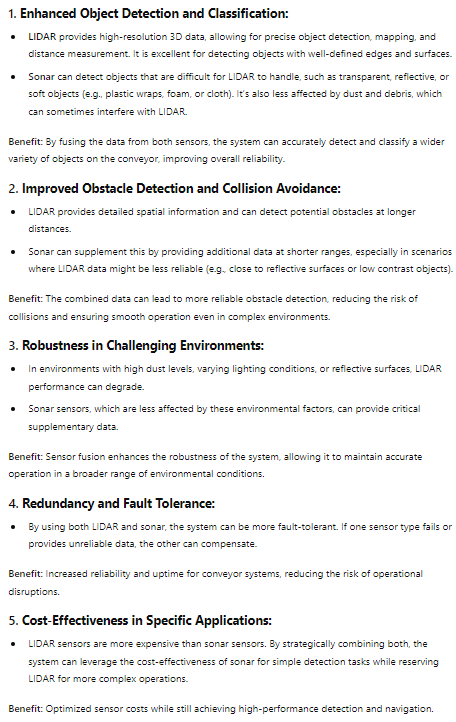
\includegraphics[width=0.5\textwidth]{./Images/chatgpt1.png}
	\caption{\label{fig:chatgpt1}ChatGPT compares sensing technologies}
\end{figure}

\subsection{Example 2: }

\subsection{Example 3: }
	
	% 15 pages
	\newpage
	\section{Hardware Design}
	\subsection{Rollator}
\noindent The most clear option for the choice of walker frame, to be outfitted with motors and the electronics system, is a standard medical rollator, available on common online commercial marketplaces. The model of choice is the Medline Premium Empower Rollator. The steel frame remains at a weight under 20 pounds, and its dimensions are given as 23.8"D x 11"W x 22"H. It comes with a seat, storage compartment, and pneumatically actuated brakes. The FORWARD team plans to remove the seat and storage compartment to replace with the electronics housing, change the braking system to velocity control, and to dismount the wheels to install the DC motors. The wheels are also 8 inch diameter, which we anticipate will provide enough torque for the adaptive velocity control and steering enacted by the motor shield.\\

\begin{figure}[H]
	\centering
	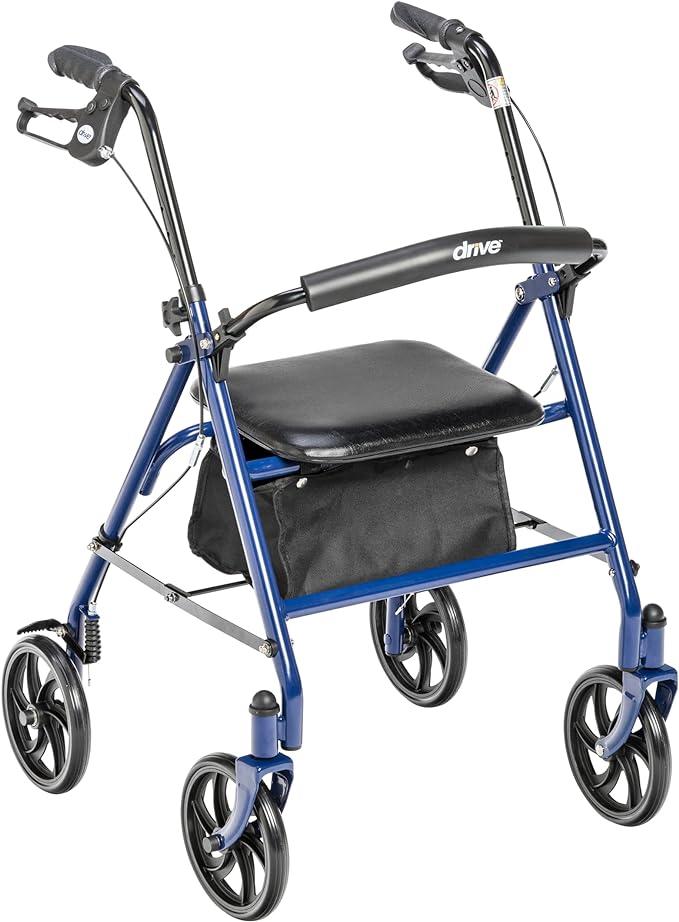
\includegraphics[width=0.3\textwidth]{./Images/rollator-amaz.jpg}
	\caption{\label{fig:rollator-amaz}Medline Premium Empower Medical Rollator}
\end{figure}

\noindent There are many other variants of rollators available - some with enlarged front wheels and some with only three wheels altogether. There seem to be two main shapes of frame: A and what we can call $\lambda$. We estimate that, the A frame is more appropriate for our purposes. FORWARD velocity control and electric braking also requires four wheels.\\

% morgan - do we fix the wheels in place? most of them swivel like castors

% matthew
\subsection{Electronics Chassis} \label{chassis}
% Discuss psychical location of all elements and components on the walker frame and explain the reason. explain plans for wiring and attachment (tape, glue, screws etc).
\subsubsection{Location of Components}
\noindent The diagram below depicts the physical location of the components as attached to the walker. Several components, including the power supply, Bluetooth module, PCB, IMU, and LiDAR will be housed within a hard casing, most likely made of metal or wood. They will be encased so that they are stable and not exposed to the elements. The LiDAR and IMU, both of which are mounted to the PCB, should not be allowed to change position. In particular, the IMU measures the angle of the walker and needs to be level. If the IMU is not level, it will give incorrect readings. It is also undesirable for the PCB to be unstable or mounted loose beneath the seat because it would be easy for connections to loosen or for vibration to damage sensitive parts. We will use screws to mount the internal components to this casing so that all of the units are fixed in place. All of the other components will need to have wires running to this casing. These wires will be organized and mounted against the walker using wire clips so that there are no dangling wires, which could be a tripping hazard to the user and would appear unprofessional.\\

\noindent For the components installed apart from the electronics case, we will use different methods of mounting depending on the nature of the component. The haptic motors will be located underneath the handlebars so that the user's hands are able to clearly sense the pattern of vibration. Each motor will be attached using a mounting bracket. This bracket will need to use tension or compression in order to secure the motors in place as the motors do not come with holes to mount to the back of the seat with screws. The headlight will be mounted on top of the backing of the walker seat. This location was chosen because it is the highest point of mounting for which the light can shine unobstructedly. It comes with a mounting bracket that will need to be attached to the walker using screws. The photoresistor may be attached to the headlight, out of the way of shadows, using a clip. There are four ultrasonic sensors that we will mount to the legs of the walker. Two will appear facing the front of the walker and the other two will appear on the side, angled toward front. The ultrasonic sensors contain small holes at each corner for mounting, however, it would be difficult to drill into the metal structure of the walker. We could use fishing rod clips to attach to the walker and mount the sensors to the clips.\\

\noindent The most difficult components to mount will likely be the DC motors driving the wheels. We must attach the motors in such a way that the wheel rotates as the rotor attached to the gearbox rotates. We also must ensure that the manual braking system is not eradicated, which limits our options to not mount the motor directly above the wheels. For example, we could detach the wheels from the hub and attach them directly to the motors whereas the motors are mounted to the walker. However, this would remove the braking mechanism from the wheels. Thus, we will mount the motor (using a connector piece screwed into the gearbox and the rim of the wheel) to the outside of the wheel and simply use a custom metal bracket to attach the motor to the leg of the walker. We will mount the two motors to the two rear wheels of the walker, as they are fixed, while the front two wheels swivel.\\ 

\begin{figure}[H]
	\centering
	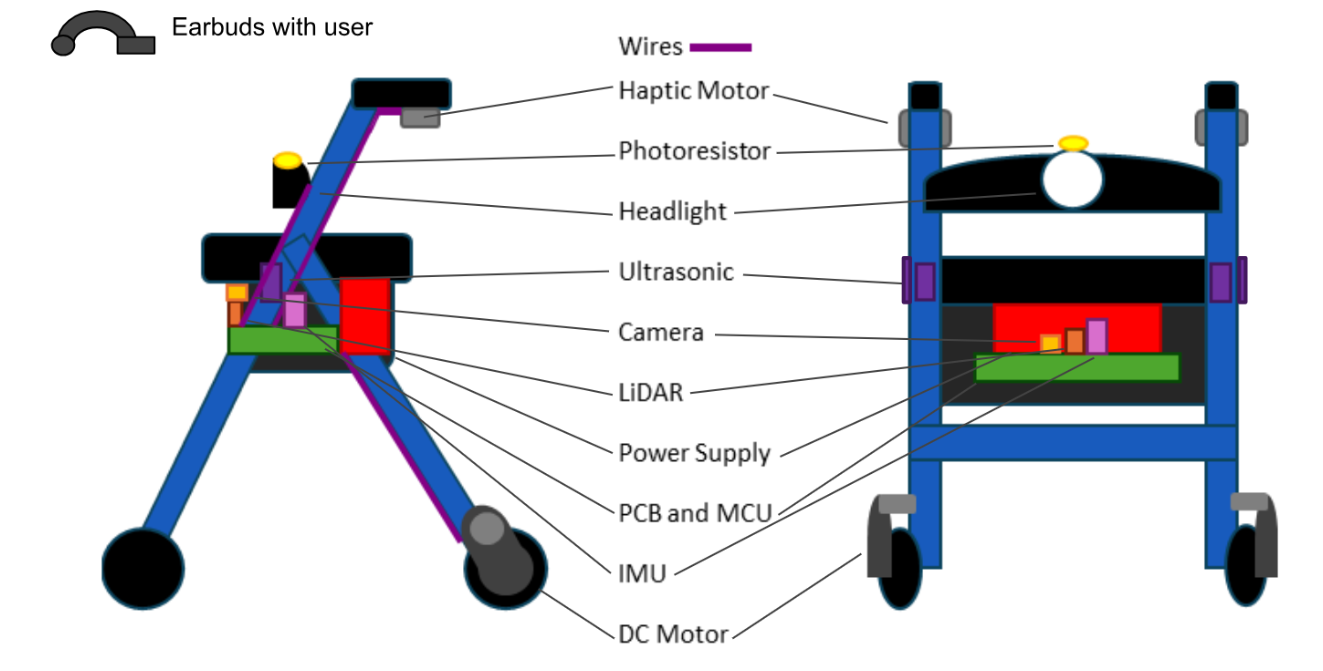
\includegraphics[width=1\textwidth]{./Images/component_location_ear.png}
	\caption{\label{fig:Component-Locations}Location of components on the walker}
\end{figure}

\subsubsection{Measurements of the Walker}
\noindent Upon purchasing the rollator chassis, we took measurements in order to design the placement of components on the walker. This is especially essential for obtaining the correct length of wires. We would like to have organized wires flush against the walker running from the PCB to different components, which requires precise measurements of the length of wires to appear professional. For example, we measured the distance from the wheel to the seat of the walker and will need to later add the measurement from the seat to the PCB housing underneath the seat. For Senior Design II, we will need the measurements for the PCB before we can start ordering the correct length of wires.\\

\begin{figure}[H]
	\centering
	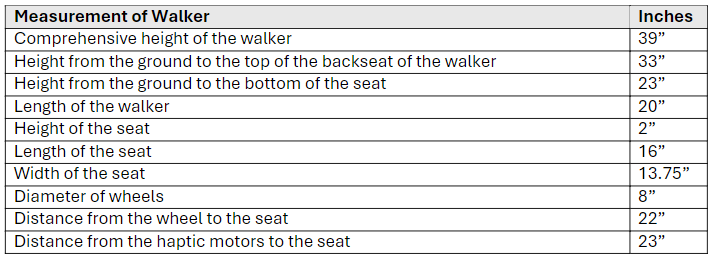
\includegraphics[width=1\textwidth]{./Images/measurements.png}
	\caption{\label{fig:Measurements_of_walker}Measurements of the walker}
\end{figure}

\noindent implementation of earpiece being available to user. physical object avoidance margins. obstacle classifications.\\

\noindent headlights? curb assist? tipover prevention with motors explained\\
	\subsection{Arduino}
\noindent Initial interfacing to the sensors was performed using the Arduino integrated development environment with an Arduino Uno board. Because of its ease of access and abstraction, this has become the preferred programming tool for the FORWARD system. The Arduino IDE has the built-in serial plotter, which can be integrated with MATLAB for use of a polar plot showing the field-of-vision. The Arduino IDE will continue to be used as a development tool going into Senior Design II, while the Arduino Uno will not, as the FORWARD team fully transitions to the ESP32.\\

\subsection{Detection Subsystem}
\noindent Recall the requirements of the detection subsystem. It should be able to detect objects at least 3 meters away and within a 15 degree aspect angle. It also should detect walker instability up to 10 degrees in pitch angle. It should detect hazards with an accuracy of at least 80\%. Finally, feedback latency should not exceed 100 milliseconds to keep the user safe.\\

\noindent Let us also define the input and output of the obstacle detection subsystem. The input is energy return from the environment, supplied to 5 different points on the walker frame, as well as accelerometer and magnetometer data outputs describing the attitude of the walker itself. The output is somewhat joint with the obstacle identification system, as it helps to generate velocity motor commands for both speed and turn angle. Detection and identification are the FORWARD system inputs, and avoidance is the output.

\subsubsection{Addressing Stretch Goals}
\noindent The range sensors are mounted on the frame perpendicularly to obstacles. In other words, the direction of the energy transmitted is perpendicular to the ground. However, the question of maximizing capability of detecting obstacles at the wheel level, and to prevent ignorance of more dangerous and deceptive hazards such as ledges or step-downs is raised. The monostatic ones will be mounted on the legs near the wheels, front-facing, while the multistatic are used for lateral detections.\\

\noindent To achieve \textit{curb lifting}, we rely on successful classification of an approaching ledge scenario by the recognition image processing, which we foresee could be challenging due to the non-distinctness of curbs, and the difficulty the sensors will have detecting them. When the front wheels are about to make contact, we can use the audio feedback to prompt the user to push down on the handlebars to raise the front wheels, then also give haptic feedback once they have placed them onto the new ground. The user is then prompted to move forward, raising the rear wheels and placing them atop the curb in the same manner as before, confirmed by haptic vibrations.\\

\noindent To achieve \textit{tipover stabilization}, we can monitor for a sudden positive delta in the pitch angle reading of the IMU. It's rate of change would need to be fast enough to distinguish from merely a change of terrain, when in fact, the user is still stable. The rapid change of pace means the user has fallen forwards while still holding the handlebars. By applying the emergency brake, friction between the rear wheels (the front wheels have reared up) can help convert the rollator into a crutch. Potentially, commanding the motors to spin backward to prop the user up to brace their fall could work too, but intense testing is required.\\

\subsubsection{Incline and Decline Stability}
\noindent The simple function fulfilled by the inclusion and integration of the IMU is stability. By monitoring the pitch angle of the walker, we know whether the user is at risk of falling over.\\

\begin{figure}[H]
	\centering
	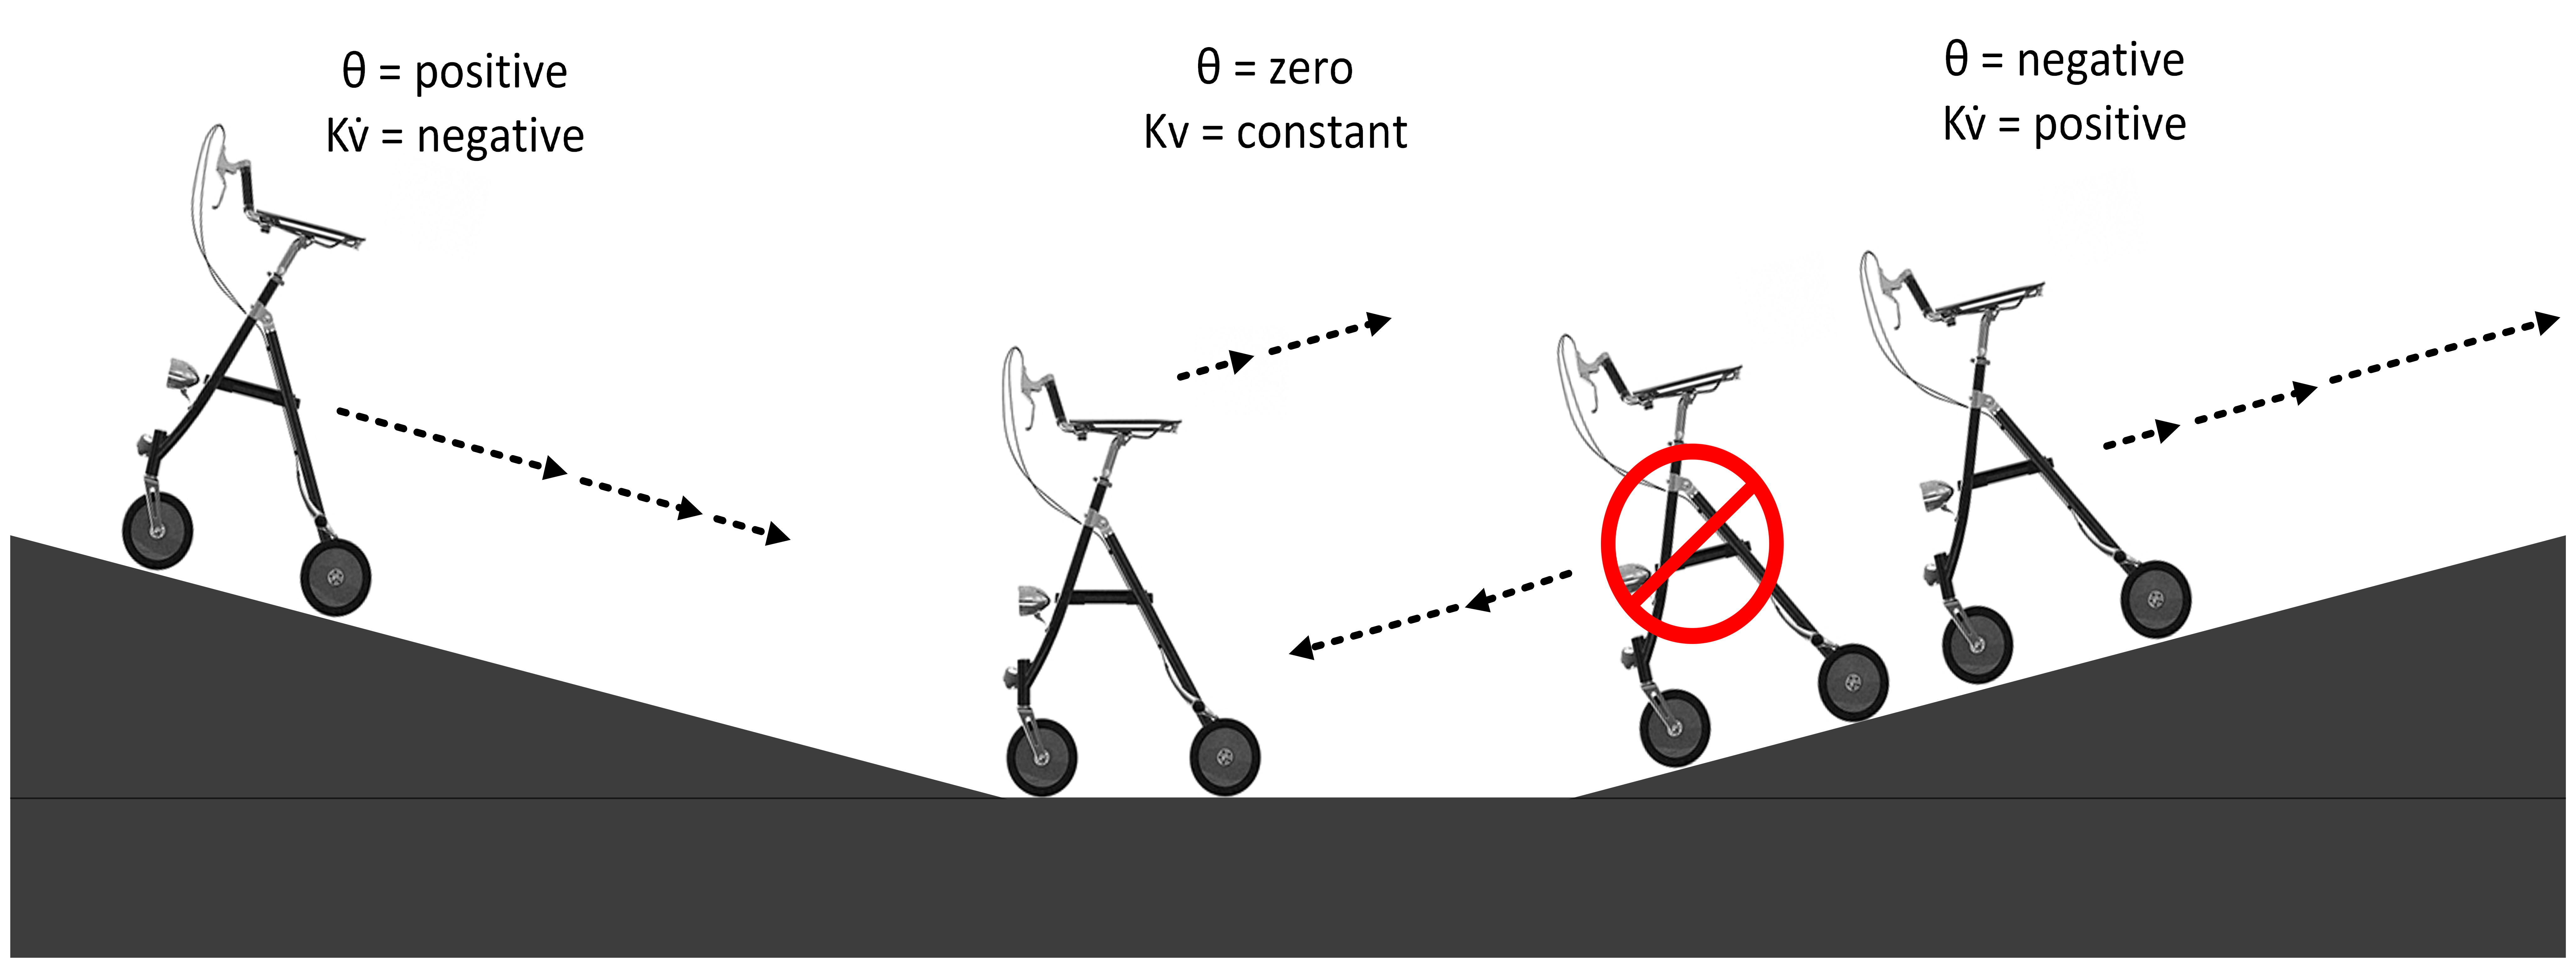
\includegraphics[width=\textwidth]{./Images/Incline-Decline-Stability.png}
	\caption{\label{fig:slope-stability}Stability on Slopes}
\end{figure}

\subsubsection{Sensor Fusion}
\noindent How do we make sense of the range detection made at all five points of the front-face of the walker? How do we combine that with pixel data of the corners of an object detection made by the camera? We can generally perceive depth by averaging the 4 coordinates, where closer is a higher average. We also know whether an obstacle is on the left or right side ahead based on which ranges are lower the maximum. We have to take into account the dead zones. With all of this information available on the network, we can build algorithms to guide the way forward, as discussed in the following chapter.\\

\noindent As noted, the ESP32 development board supports all the sensors and the camera simultaneously without the need of multiplexing. The setup pictured below in figure \ref{fig:bb-test} has the IMU and LiDAR on an I2C bus, and the ultrasonic sensors routed to GPIO pins. A table of the varying assignments, labels, and voltage requirements would be provided for the topology in figure \ref{fig:bb-test}, but it is forbidden by the UCF ECE guidelines. Suffice it to say, the IMU requires 3.3V, the TFLuna LiDAR requires 5V, and both variants of the ultrasonic can support either voltage.\\
\begin{figure}[H]
	\centering
	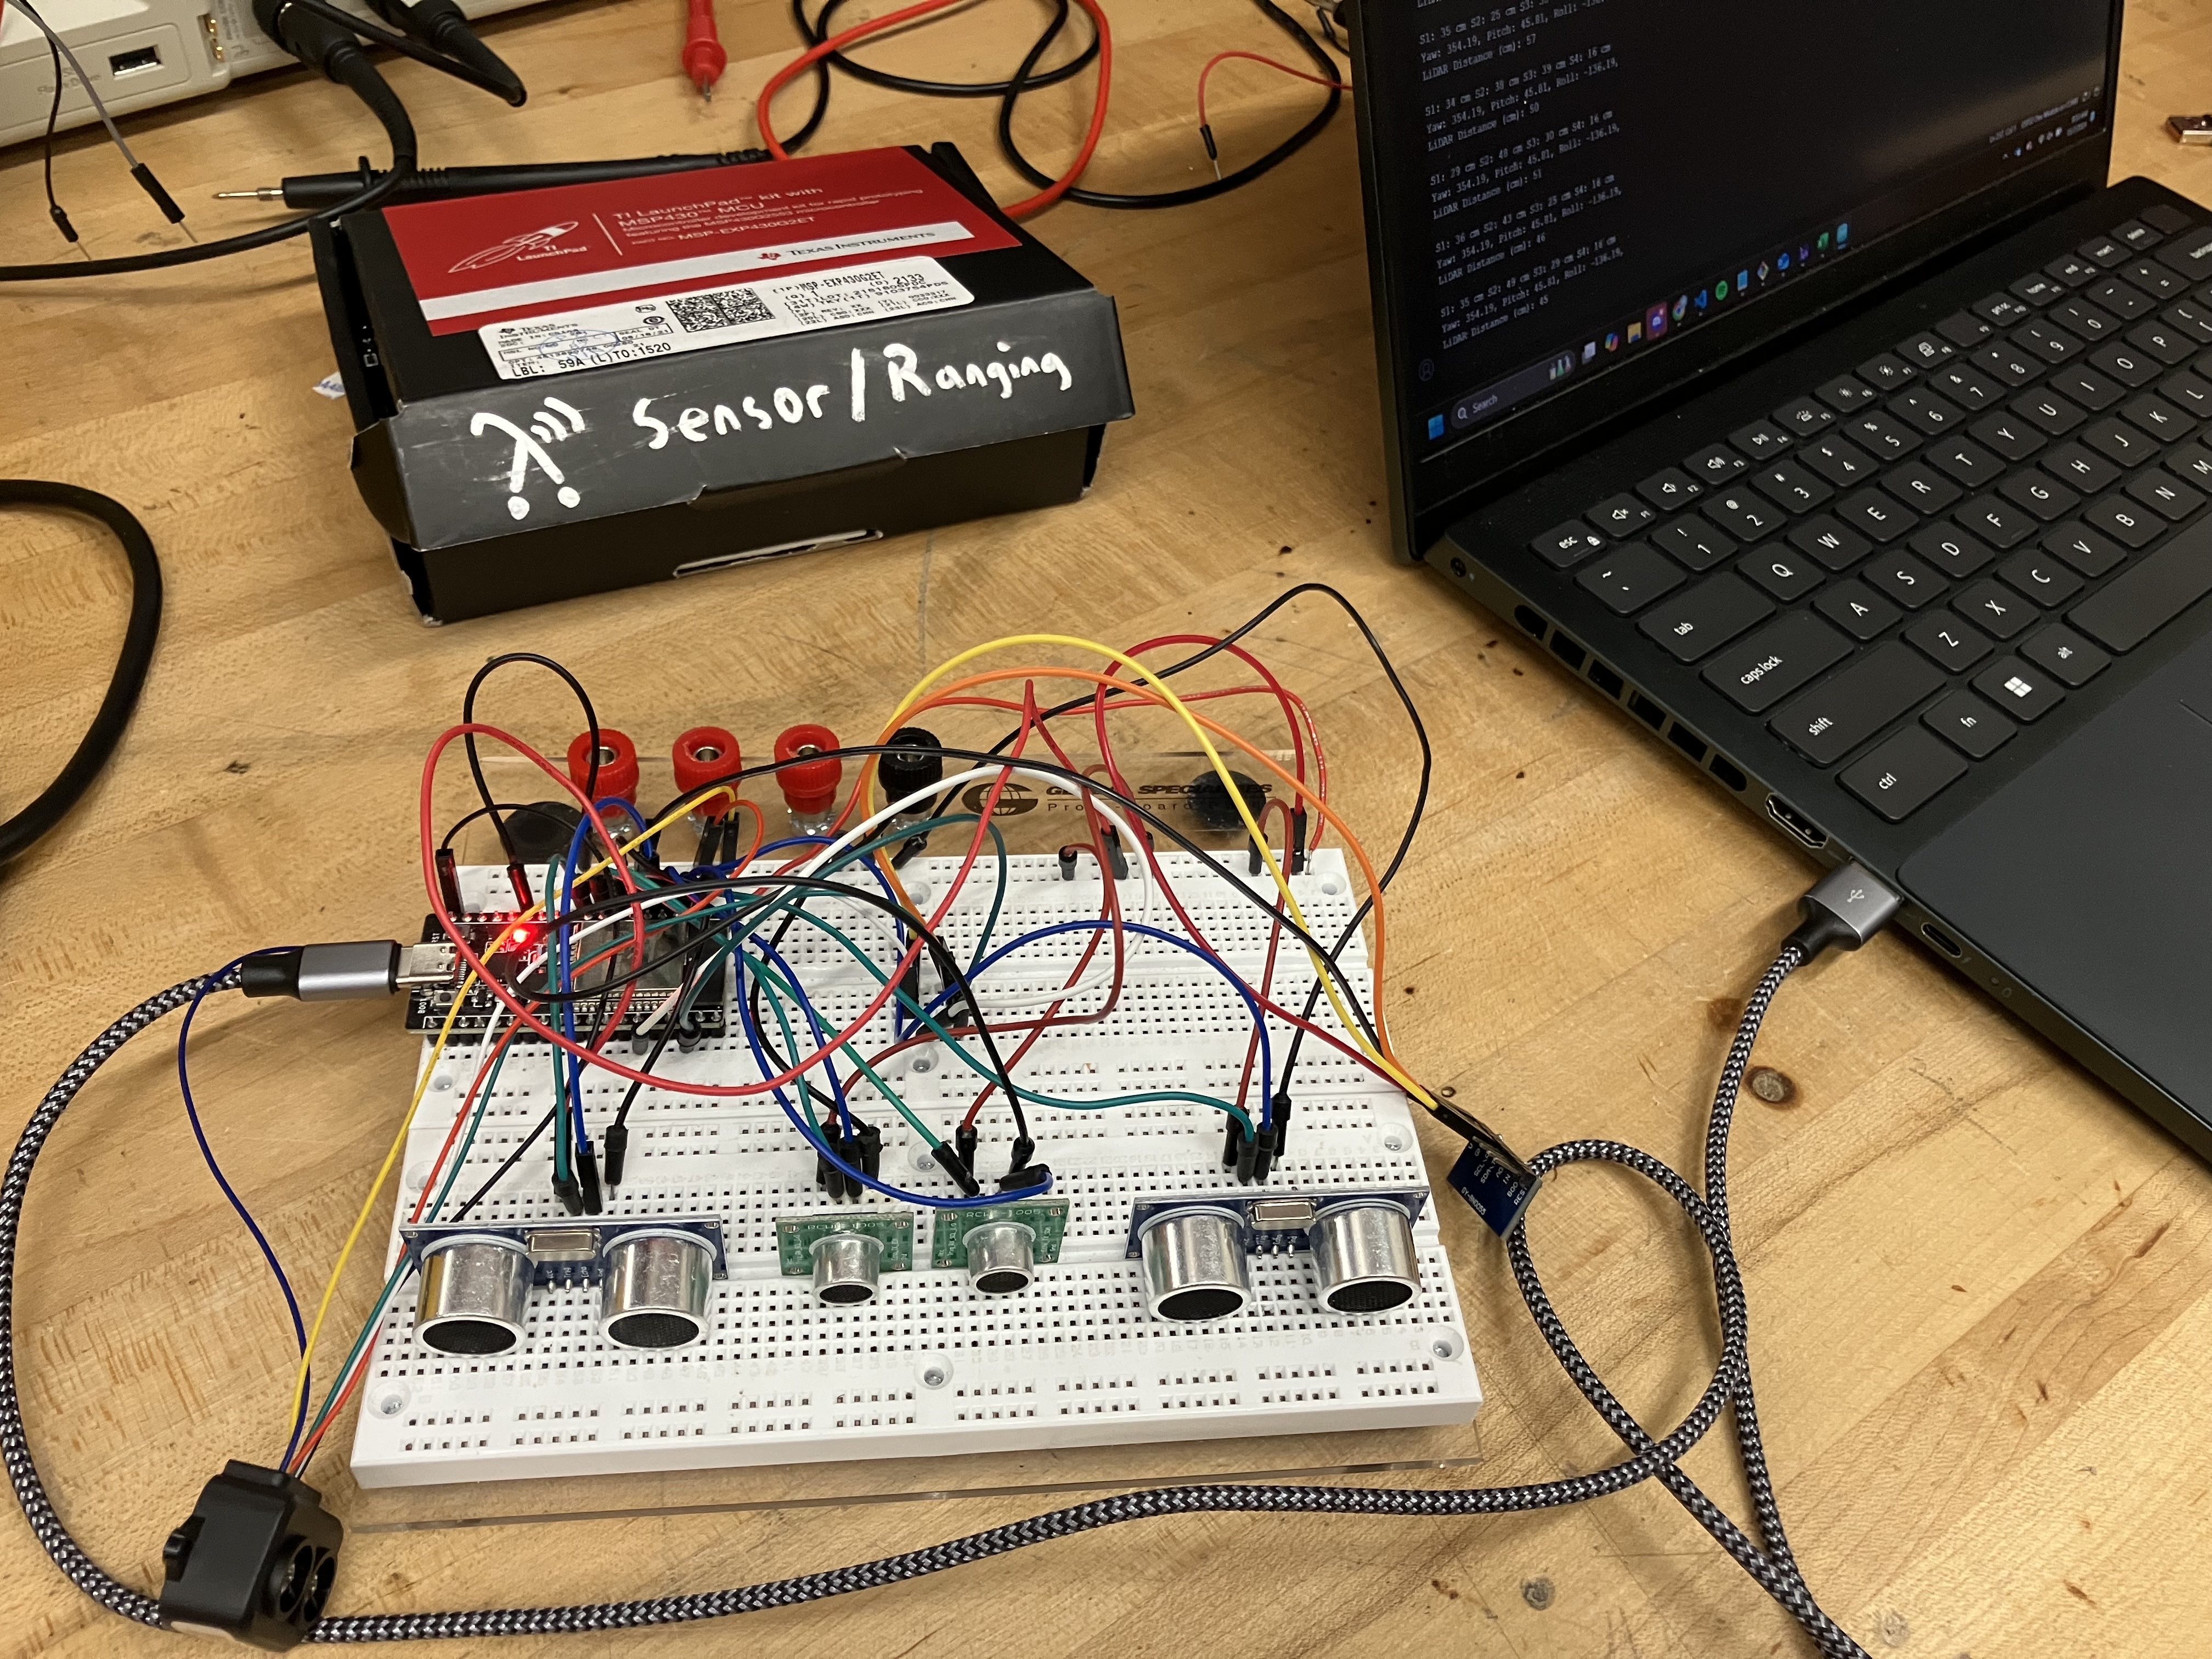
\includegraphics[width=0.5\textwidth]{./Images/breadboard-test.jpg}
	\caption{\label{fig:bb-test}Breadboard w/ Ultrasonics, and IMU \& LiDAR I2C Bus}
\end{figure}

	\subsection{Identification Subsystem}
% intro paragraph

% how is the ESP32 able to host its own wireless network. confirm we don't require FORWARD to be connected to a WIFI network or personal hotspot.
\subsubsection{ESP32 Wireless Network}
\noindent Antenna?
	\subsection{Power Supply and Voltage Regulation}
\noindent Each component of the FORWARD walker requires a specific amount of voltage. In order to cater to each of these needs, we will first need to have separate power supplies. The motors driving the wheels as well as the headlight both demand 12V, so they will require a larger power supply that only outputs 12V. The remainder of the components, contrarily, all use a much smaller power supply. Thus, we will utilize a large power supply and a small power supply (both of which are rechargeable).\\

\noindent For the smaller power supply, we will need to employ voltage regulation to provide the correct amount of voltage between the different units. The microcontroller and accompanying sensors all require one voltage supplied to the MCU and distributed to the sensors. The ESP32 is rated as a 3.3V device\cite{sparkfun12024} and powers the sensors using the GPIO pins. However, the haptic motors require a separate power supply from the MCU as they are operated using a motor driver rated for 5V. The camera module is also powered separately from the MCU with a supply of 5V. In order to deliver enough voltage for both the MCU, the camera module, and the haptic motors, we will use a 5V battery pack (originally designed to charge phones) and from there add voltage regulation circuits to the PCB. The haptic motors and the camera module will accept the simple output of the battery pack at 5V, however, the MCU and its sensors will need this voltage to be stepped down 3.3V. This circuit will be implemented within the PCB.\\

\subsection{Avoidance Subsystem}

\noindent This subsystem is dedicated to the movement of the walker as pertains to the motors and mechanics. FORWARD has a prescribed method of steering and braking that will be expanded upon. There have also been changes to the design throughout the project affecting our choice and application of the motors to be discussed.\\
% intro paragraph

% do we fix the wheels in place? most of them swivel like castors - that's fine, rear-wheel drive.
\subsubsection{Wheel Rotational Motion}
\noindent The rollator wheels will dictate the way by which turning can be achieved. There are four wheels. We call the distance in between the front wheels $axel_f$ and the distance in between the rear wheels $axel_r$. Upon initial inspection of the rollator once acquired, we see that $axel_f > axel_r$. The measurements are as follows:\\

[TABLE HERE OF MEASUREMENTS]\\

\noindent From a top view, the rear two wheels can be viewed as simple points. They do not swivel, and thus can rotate in place but cannot do horizontal translation, stipulated by friction and attachment to the rollator frame. Of course, they can also roll and move forward.\\

\noindent In addition, the front wheels are on a $360^{\circ}$ swivel. They can also be modeled as points in a sense; however, their orientation changes.\\

\noindent \underline{\textit{Case 1}} (extreme): Both wheels rotate. The front wheels translate.\\

[INSERT CASE 1 DIAGRAM FROM POWERPOINT ONEDRIVE HERE]

\noindent \underline{\textit{Case 2}} (extreme): one wheel rotates, the other stationary. The front wheels revolve.\\

[INSERT CASE 2 DIAGRAM FROM POWERPOINT ONEDRIVE HERE]

\noindent \underline{\textit{Case 3}} Veering. motor speeds may not have to change. User can veer based on feedback, and gentle guidance provided by FORWARD.\\

[INSERT CASE 3 DIAGRAM FROM POWERPOINT ONEDRIVE HERE]

% talking more about one wheel motor faster than the other. fusing user steering with FORWARD guidance.\
\subsubsection{Turning Mechanics}
\noindent A major question pertaining to obstacle avoidance is our mechanism of steering. As mentioned previously in section 3.2.7, we wish to rely solely on the DC motors for steering control in order to minimize mechanical complexity.  To refresh, rather than using a servo motor or other apparatus to turn an axle that steers the wheels, we will use two separately controlled DC motors with no axle. Because each of these motors are controlled independently, each will assume a different speed in order to steer the wheels, else remain at equal speeds to move forward in a straight line. The angle of the turn is determined by the drop in speed of the motor adjacent to the turning direction. As an example, if the walker needs to veer very sharply to the left, the left motor will either halt rotating or rotate very slowly compared to the right motor. On the contrary, if simply a slight turn is needed to avoid an obstacle, both motors will drive at comparable speeds with one motor slightly decreased in speed. One potential issue with this strategy is that FORWARD can only move in a straight line if both motors are rotating at exactly the same speed; otherwise, the walker may drift toward one side or the other, as opposed to an axle that is driving the wheels symmetrically. However, we are using identical motors from the same manufacturer and applying the same amount of voltage. It is possible that there will still be some amount of drift due to manufacturing errors, wire resistance, or other unknown factors. Nonetheless, we do not anticipate drift to be much of an issue as the walker can also correct itself upon straying from the path, as it will detect an obstacle, whether the obstacle is a curb, the grass, the road, etc.\\

% what methods and considerations do we have when sticking the motors on the rollator?
\subsubsection{Motor Installation}
% reconciling measurements acquired of the wheel diameter, weight, etc, with the torque of the DC motors.
\noindent \underline{\textit{Calibration}}\\
\noindent Our initial selection for DC motors driving the wheels were the S55B-150 motors from Chapter 3. However, there were several factors that we did not account for in purchasing these motors. To begin with, these motors are brushless three-phase DC motors. After discussing with Dr. Weeks, one of our coordinators for Senior Design, we learned that in order to program these motors to function properly, each of the phases needs to be aligned within the programming. This would be a very difficult process, especially considering that there is hardly any documentation given for the S55B-150 given by the seller. In considering this advice, we purchased instead \cite{amazon12024}. Although these motors are only 40-50W, they nonetheless provide plenty of torque to drive the walker due to the gearbox increasing torque. We will eventually need to test the speed of the walker to see if it will be able to achieve one of our requirements of 6mph. The motors with no load can rotate up to 30,000rpm, which with 8" diameter wheels translates to over 700mph \cite{lucidar2024}. However, this number will drastically change as up to 60lbs plus the weight of the user's body leaning against the walker acts as a large load. We will simply need to test the speed of the walker in Senior Design II and keep in mind that speed may not be a requirement that is met.\\


% does simply glueing the haptic motors on the handlebar underside sufficiently vibrate the handlebars to where the user notices? how much power would that require?
\noindent \underline{\textit{Vibrating Handlebars via Haptics}}\\

\noindent Our design for haptic feedback includes small ERM motors that will spin at a rapid rate with no load. Attached underneath the handlebars to the walker, the rapid spinning will cause a vibration noticeable to the user. This is a vital portion of guidance to the user, as our desire with this project is to provide a solution for people with a broad range of sensory disorders. If the user has issues with using the audio feedback or is unable to hear, the haptic motors provide similar directions describing the surroundings and motion of the walker. When our FORWARD walker detects and identifies obstacles, the user must be aware that an obstacle has been detected, what the obstacle or danger level is, and what steps the walker will take in order to avoid the obstacle. Otherwise, the user may act contrary to the walker or stumble in response to the sudden change in movement. For example, if FORWARD approaches a wall and comes to a stop, the user, who is walking with the walker, could run into the walker or be lunged forward by inertia apart from feedback.\\ 

\noindent The haptic motors are being controlled by a motor driver communicating with the ESP32. This motor driver receives commands from the ESP32, which also combines input from the various sensors, and sends commands to the motors that vibrate accordingly. When an obstacle is initially detected, the motor on the side in which the obstacle is detected will vibrate in pulses until it is time for FORWARD to either steer or brake to avoid the obstacle if needed. If the walker needs to veer to the right or to the left in response to the obstacle, the handlebar in the direction the walker is steering toward will vibrate for the duration of the turn. The ERM motors will vibrate in pulses while the walker is turning, with the period of the pulses dependent on the steering angle. If FORWARD needs to take a sharp turn, the haptics will vibrate more often with shorter pulses, whereas a slight turn will vibrate with longer pulses. If FORWARD is coming to a stop, both haptic motors will vibrate simultaneously until the walker has come to a complete stop. After a short delay, perhaps around five seconds, if the obstacle passes, both of the haptic motors will vibrate twice for around one second per pulse to indicate the walker will move forward again. The motion will begin after this warning is given to the user. If the obstacle does not pass but instead FORWARD needs to turn away from the obstacle after coming to a complete stop, one haptic motor will vibrate twice for around one second per pulse on the side in which the walker is turning toward.\\ 

\noindent Considering the data captured and processed by the camera, we also need a way for the user to distinguish between different obstacles. The system of haptic feedback will accomplish this using pulse width modulation (PWM). PWM is a method of speed control discussed in section 3.2.6 where voltage is applied for a percentage of a period. When the high voltage pulses are wider (the motors are spinning at a faster rate), the haptic motors vibrate louder, whereas a shorter voltage pulse results in weaker vibration. Because a louder vibration draws more attention, a sense of urgency is conveyed. Thus, we will use the speed of vibration to indicate the danger of the approaching obstacle. We will first classify each of our recognized obstacles with a danger level (for example, a vehicle most dangerous, then a human, and grass least dangerous) and set the speed of the motors accordingly.\\

% talk about how the rollator has pneumatic handle squeeze brakes but braking can also be achieved by locking the DC motors
\subsubsection{Emergency Braking}
\noindent FORWARD of necessity must also be able to respond to obstacles by braking. The chassis we have chosen to use already contains a manual braking system. There are pneumatic triggers beneath the handlebars that apply the brakes upon compression. We would like to preserve these manual brakes for the sake of safety in case any electrical or software issues arise. However, we also need FORWARD to brake automatically in response to obstacles. We will accomplish this by programming the motors to first slow down their speed to a stop and then reverse the direction of the motors until the entire walker is no longer in motion. This is known as dynamic braking\cite{electricaleasy2014}. We will need to test the braking to determine the correct timing of when the walker comes to a complete stop so that we know when to stop the motors after reversing. If we are unable to correctly time the motors, we may need a way to sense when the walker has come to a complete halt. This may be possible using the camera or a motion sensor \cite{bayalarm2024}.\\

%issue about user trying to steer when they shouldn't
\subsubsection{Reconciling User Control and Automatic Guidance}
\noindent There is also an issue of user error that must be considered. Our design is intended for the walker to lead the user, not for the user to lead the walker. This is not much of an issue with braking as there should not be any safety issues in the user applying manual brakes when not needed. Although this may wear down the motors over time as the rotor is prevented from rotating, we do not foresee any major consequences. However, the user may try to steer the walker in the wrong direction when not directed by the walker. This could cause a serious issue in the safety of the user if they steer the walker into an obstacle. Currently, if the user tried to steer the walker, the walker would automatically correct itself upon encountering an obstacle and warn the user of the obstacle. A more advanced solution could be pressure sensors that detect the body weight of the user and can sense if the user is leaning a particular way. However, this is outside the scope of our project, although in production this issue would certainly need to be addressed.\\ 

	
	% 15 pages
	\newpage
	\section{Software Design}
	\subsection{Guidance, Navigation, and Control Software}
\noindent GNC situation, tilt (attitude) using IMU, (incline decline), velocity and position solutions, ESP32 source code GitHub (hc-sr04.c luna.c haptic.c audio.c motor.c ip.c avoid.c), motor commands calculation\\

\noindent UML class diagram\\

\subsection{Computer Vision}

\subsection{Serial Interface}

\subsection{Motor Control Software}
	\subsection{Ranging Algorithms}
\noindent Instructing FORWARD where to guide the user is a solution that the detection and identification systems generate. Various scenarios are described in the system testing chapter. It will be a matter of solving an adaptive geometrical situation and relaying the results to the processor.\\

\subsubsection{State Space Representation}
\noindent There are more outputs the inertial measurement unit can provide besides the angles. One of most interesting ones is the accelerations. This would be the rate that the velocity of the rollator body is changing with respect to time. From a control standpoint, we can think of a state-space representation. FORWARD is a multi-input, multi-output system (MIMO). Let's define the states:
X and Y position (2D plane on the ground), yaw angled orientation, x and y velocity, and the angular velocity:
$$X = [x, y, \theta, v_x, v_y, \omega]^T$$
The inputs are the yaw angle steering command and the left and right motor spin speeds:
$$U = [\phi, u_l, u_r]^T$$
The outputs are the range sensor readings, the IMU acceleration, and Euler angles:
$$Y = [s_1, s_2, s_3, s_4, l_1, a_x, a_y, a_z, \alpha, \beta, \gamma ]^T$$

\noindent The state equation, where differential operators, and various constants determine the relationships. $\epsilon_n$ is a very small value, meaning the difference between the two variables should be minimized. $k_n$ is a motor coefficient, in which the steering is determined by the differential wheel spin between left and right motors:
\[\dot{x} =
\begin{bmatrix}
	\dot{x}\\ \dot{y}\\ \dot{\theta}\\ \dot{v_x}\\ \dot{v_y}\\ \dot{\omega}\\
\end{bmatrix} = 
\begin{bmatrix}
	1 & 0 & 0 & \frac{d}{dt} & 0 & 0 \\
	0 & 1 & 0 & 0 & \frac{d}{dt} & 0 \\
	0 & 0 & 1 & 0 & 0 & \frac{d}{dt} \\
	0 & 0 & 0 & \frac{d}{dt} & 0 & 0 \\
	0 & 0 & 0 & 0 & \frac{d}{dt} & 0 \\
	0 & 0 & \frac{d}{dx}\frac{d}{dy} & 0 & 0 & \frac{d}{dt} \\
\end{bmatrix}
\begin{bmatrix}
	x\\ y\\ \theta\\ v_x\\ v_y\\ \omega
\end{bmatrix} + 
\begin{bmatrix}
	\frac{d}{dt} & \frac{d}{dt} & \frac{d}{dt} \\
	\frac{d}{dt} & \frac{d}{dt} & \frac{d}{dt} \\
	\epsilon_1 & k_l & k_r \\
	0 & \epsilon_2 & \epsilon_3 \\
	0 & \epsilon_4 & \epsilon_5 \\
	\frac{d}{dt} & 0 & 0\\
\end{bmatrix}
\begin{bmatrix}
	\phi\\ u_l\\ u_r
\end{bmatrix}
\]

<<<<<<< HEAD
\subsubsection{Range Reading Harmonization}
\noindent In order to properly utilize all of the data our peripherals supply, we must design an effective and efficient sensor fusion system that can harmonize all of the incoming sensor data with the object detection data. In our research, we referenced an article \cite{CVRef2} that discussed using a 2D grid to determine where objects were in space. We are going to bring these ideas into our design, but allowing the object data, which comes with a position on a 2D-grid, to set this grid, which then our sensors can be associated to certain sections of this grid to provide ranging. For our purposes, x = 1920 and y = 1080 because our camera has a 1920x1080 frame size. We also know that the origin (0,0) is at the bottom left from the perspective of the camera. In figure \ref{fig:proposedsensorFOV}, we see that we will have four sonar sensors surrounding FORWARD. To illustrate my point, if we had an object return the position (1200, 1800, 0, 800), this being the form (Xmin, Xmax, Ymin, Ymax), then we would trigger the front right sonar sensor and receive the ranging measurement of said object. \\

\noindent We will also utilize the LiDAR readings to provide more precise ranging... \\

\noindent There are more outputs the inertial measurement unit can provide besides the angles. One of most interesting ones is the accelerations. This would be the rate that the velocity of the rollator body is changing with respect to time. 
=======
\noindent The relation of outputs to states and inputs is harder to determine, so the output matrix is left ambiguous (6x11):
\[y =
\begin{bmatrix}
	s_1, s_2, s_3, s_4, l_1, a_x, a_y, a_z, \alpha, \beta, \gamma
\end{bmatrix}^T = 
\begin{bmatrix}
	6\times 11
\end{bmatrix}
\begin{bmatrix}
	x, y, \theta, v_x, v_y, \omega
\end{bmatrix}^T
%\begin{bmatrix}
%	3\times 11
%\end{bmatrix}
%\begin{bmatrix}
%	\phi\\ u_l\\ u_r
%\end{bmatrix}
\]
>>>>>>> de67bcf570776e8e83ba569253c817a2855cd788


%$$X = [x_1,x_2,x_3,x_4,x_5,x_6,x_7]^T$$
%The rollator orientation (attitude, Euler angles):
%$$x_1=\psi ,x_2=\theta, x_3=\phi$$
%The rollator acceleration signals:
%$$x_4=a_x, x_5=a_y, x_6=a_z$$
%We do not consider braking or the haptic PWM signals. The main actuator signal is the yaw steering angle command:
%$$x_7=\phi_c$$
%
%\noindent The inputs $U = [u_1, u_2, u_3, u_4, u_5, u_6, u_7]^T$ are as follows. Notice roll is not dealt with because $\psi$ is static.\\
%$u_1:incline\ angle$\\
%$u_2:user\ steering\ force$\\
%$u_3:motor\ commands$\\
%Ultrasonic sensors 1-4 and the TFLuna LiDAR:\\
%$u_4:S1,u_5:S2,u_6:S3,u_7:S4,u_8:L1$
%
%\noindent The state equations:\\
%$$\dot{X} = AX + BU$$
%$$Y = CX + DU$$\\
%where D=0 because there is no direct transmission. We then can define the 7x7 state transition matrix:\\
%\[A = \begin{bmatrix}
%\alpha_1 & 0 & 0 & \beta_1 & 0 & 0 & 0 \\
%0 & \alpha_2 & 0 & 0 & \beta_2 & 0 & 0 \\
%0 & 0 & \alpha_3 & 0 & 0 & \beta_3 & 0 \\
%0 & 0 & 0 & \zeta_1 & 0 & 0 & 0 \\
%0 & 0 & 0 & 0 & \zeta_2 & 0 & 0 \\
%0 & 0 & 0 & 0 & 0 & \zeta_3 & 0 \\
%0 & 0 & \gamma_1 & \gamma_2 & \gamma_3 & 0 & 0
%\end{bmatrix}\]
%
%\noindent The control influence matrix is a 3x7 which describes the relationship of the inputs to the states:\\
%\[B = \begin{bmatrix}
%	\omega_1 & 0 & 0 & 0 & 0 & 0 & 0 \\
%	0 & \omega_2 & 0 & 0 & 0 & 0 & 0 \\
%	0 & \omega_3 & 0 & 0 & 0 & 0 & 0 \\
%	0 & 0 & 0 & 0 & 0 & 0 & 0 \\
%	0 & 0 & 0 & 0 & 0 & 0 & 0 \\
%	0 & 0 & 0 & 0 & 0 & 0 & 0 \\
%	0 & 0 & \lambda_1 & \lambda_2 & \lambda_3 & \lambda_4 & \lambda_5
%\end{bmatrix}\]

\noindent By this, we see that the state of the euler angles and accelerations are interdependent in some axes and that the yaw steering command is dependent on the yaw angle and x and y accelerations. To ensure stability, we must either minimize acceleration or maximize the range readings.\\

\noindent One important note to consider is interference of the ultrasonic pulses. Being that FORWARD uses four of them, it is important to make sure the receivers do not receive each others emitted energy reflections. Ultrasonics are directional, so by pointing the multistatic sensors to the left and right sides of the rollator to monitor passing or approaching obstacles, we decouple them from the monostatic. However, the front-facing sensors are only separated by the length of the axel, meaning these will need to be triggered sequentially to avoid interference. This can be implemented simply in Arduino by separate digital write statements.\\

\noindent This is also where a state estimator is useful. There is not a need nor a call for a mathematical definition of a Kalman filter for the scope of this project. However, we can make a general remark on the nature of the inputs and states. The sensor readings are all continuous, but can experience near instantaneous changes due to sudden appearances of obstacles or disturbances in the environment. For example, a fast moving obstacle can quickly enter the field of view, which may cause range sensor readings to drop quickly, while the amount of objects identified by the camera may change quickly as well. Therefore, an estimator is useful in the event of actively avoiding an obstacle present, in that it can help smooth response to commands and provide the best advice on where to veer toward, but it would be disrupted by the volatile environment.\\

\subsubsection{I2C Bus for Sensors}
\noindent The utilization of four ultrasonic sensors and one LiDAR to supply a feed of information to FORWARD's central processor can be integrated and realized through a wiring bus with the I2C digital communication protocol. This I2C scheme will use a synchronous clock signal provided to the sensors by the MCU. It will operate always in half-duplex, meaning data will be transmitted in only one direction at a time - from the MCU to the sensors and from the sensors back to the MCU in successive time steps. Additionally, the sensors will be accessed by their unique addresses and send packets of information as a sequence, taking turns. FORWARD does not require the use of a multiplexer device, as accessing the sensor data is done by address over the two common wires.\\
	\subsection{Identification and Image Processing}
\noindent FORWARD uses neural network technology to classify obstacles within the field of vision of the camera module.

% without copy pasting code, how does the image recognition work on the ESP cam module?
\subsubsection{Object Recognition Models}

\noindent The AMB82-MINI camera module is the board used by FORWARD to run all of the necessary object detection algorithms. In order to effectively utilize this board we first had to write the needed code. As stated above, we utilized the example object detection code provided by the board file in the Arduino IDE to guide us in this process. We opted to use a model from the YOLO family, which as the time of writing this paper is the YOLOv4 Tiny model, optimized for memory efficiency while still maintaining high performance. The YOLO model is trained on the MSCOCO data set. Once we flashed the code unto this board, the logic flow is this: 

\begin{enumerate}
	\item The camera component obtains a constant stream of image data, that is provided to the MCU via a 24-pin bus.
	\item The MCU takes this data and passes it too the model.
	\item The YOLO model then provides the output (the specific process is explained in section \ref{CV_Obj_Det})
	\item This output is then sent to the ESP32 MCU over UDP sockets over WiFi
\end{enumerate}
 

% bench, stationary car, ledge, moving person (polite obstacle avoidance), 
\subsubsection{Predetermined Obstacles}
\noindent The obstacles we have decided to avoid within the expected project scope are:
\begin{enumerate}
	\item People
	\item Benches
	\item Cars
	\item Walls
	\item Grass
\end{enumerate}

\noindent With stretch obstacles being:
\begin{enumerate}
	\item Ledges
	\item Curbs
	\item Animals
	\item Bicycles
\end{enumerate}

\noindent This means that FORWARD will be expected to avoid each of the above obstacles, handling a smooth re-navigation of the user, while keeping the user in the loop via audio feedback. The objects will be identified through our camera module and color sensor and the navigation will be accomplished by our GNC software. \\
	\subsection{Avoidance Protocols}




\subsubsection{Polite Response to Obstacle in Motion}

\subsubsection{Stationary Obstacle}

\subsubsection{Emergency Stop}
	
	% 2 pages
	\newpage
	\section{Prototype Fabrication}
	\subsection{Printed Circuit Board Design} \label{sec:pcb-design}
\noindent It is advantageous to use the 5V configuration for ESP32 UART bridge. In development, we used a development board to program the MCU but in practice must implement a UART bridge on the PCB to communicate with the MCU for flashing the memory and sending serial data out.\\

\noindent For voltage regulation, it could be expedient to, instead of using Texas Instruments Webench to design circuits for the PCB, use a 1/3 voltage divider for the ultrasonic ECHO pins. This is necessary because the ESP32 operates on 3.3V while the ultrasonic sensors use 5V, even though they are 3.3V compatible. This can be easily implemented by a 1k$\Omega$ and 2k$\Omega$ resistor in series.\\

\noindent One other consideration are the PCB traces. We intend to use 20mil (0.5mm) isolations and traces. The PCB does not use RF signals.\\

\noindent Motor controllers are more sensitive components and should be implemented on an independent PCB. These are considered as optically isolated motor drivers in order to minimize back EMI/F. In this case, one would bias an LED to turn the controller on. \cite{l293n}\\

\begin{figure}[H]
	\centering
	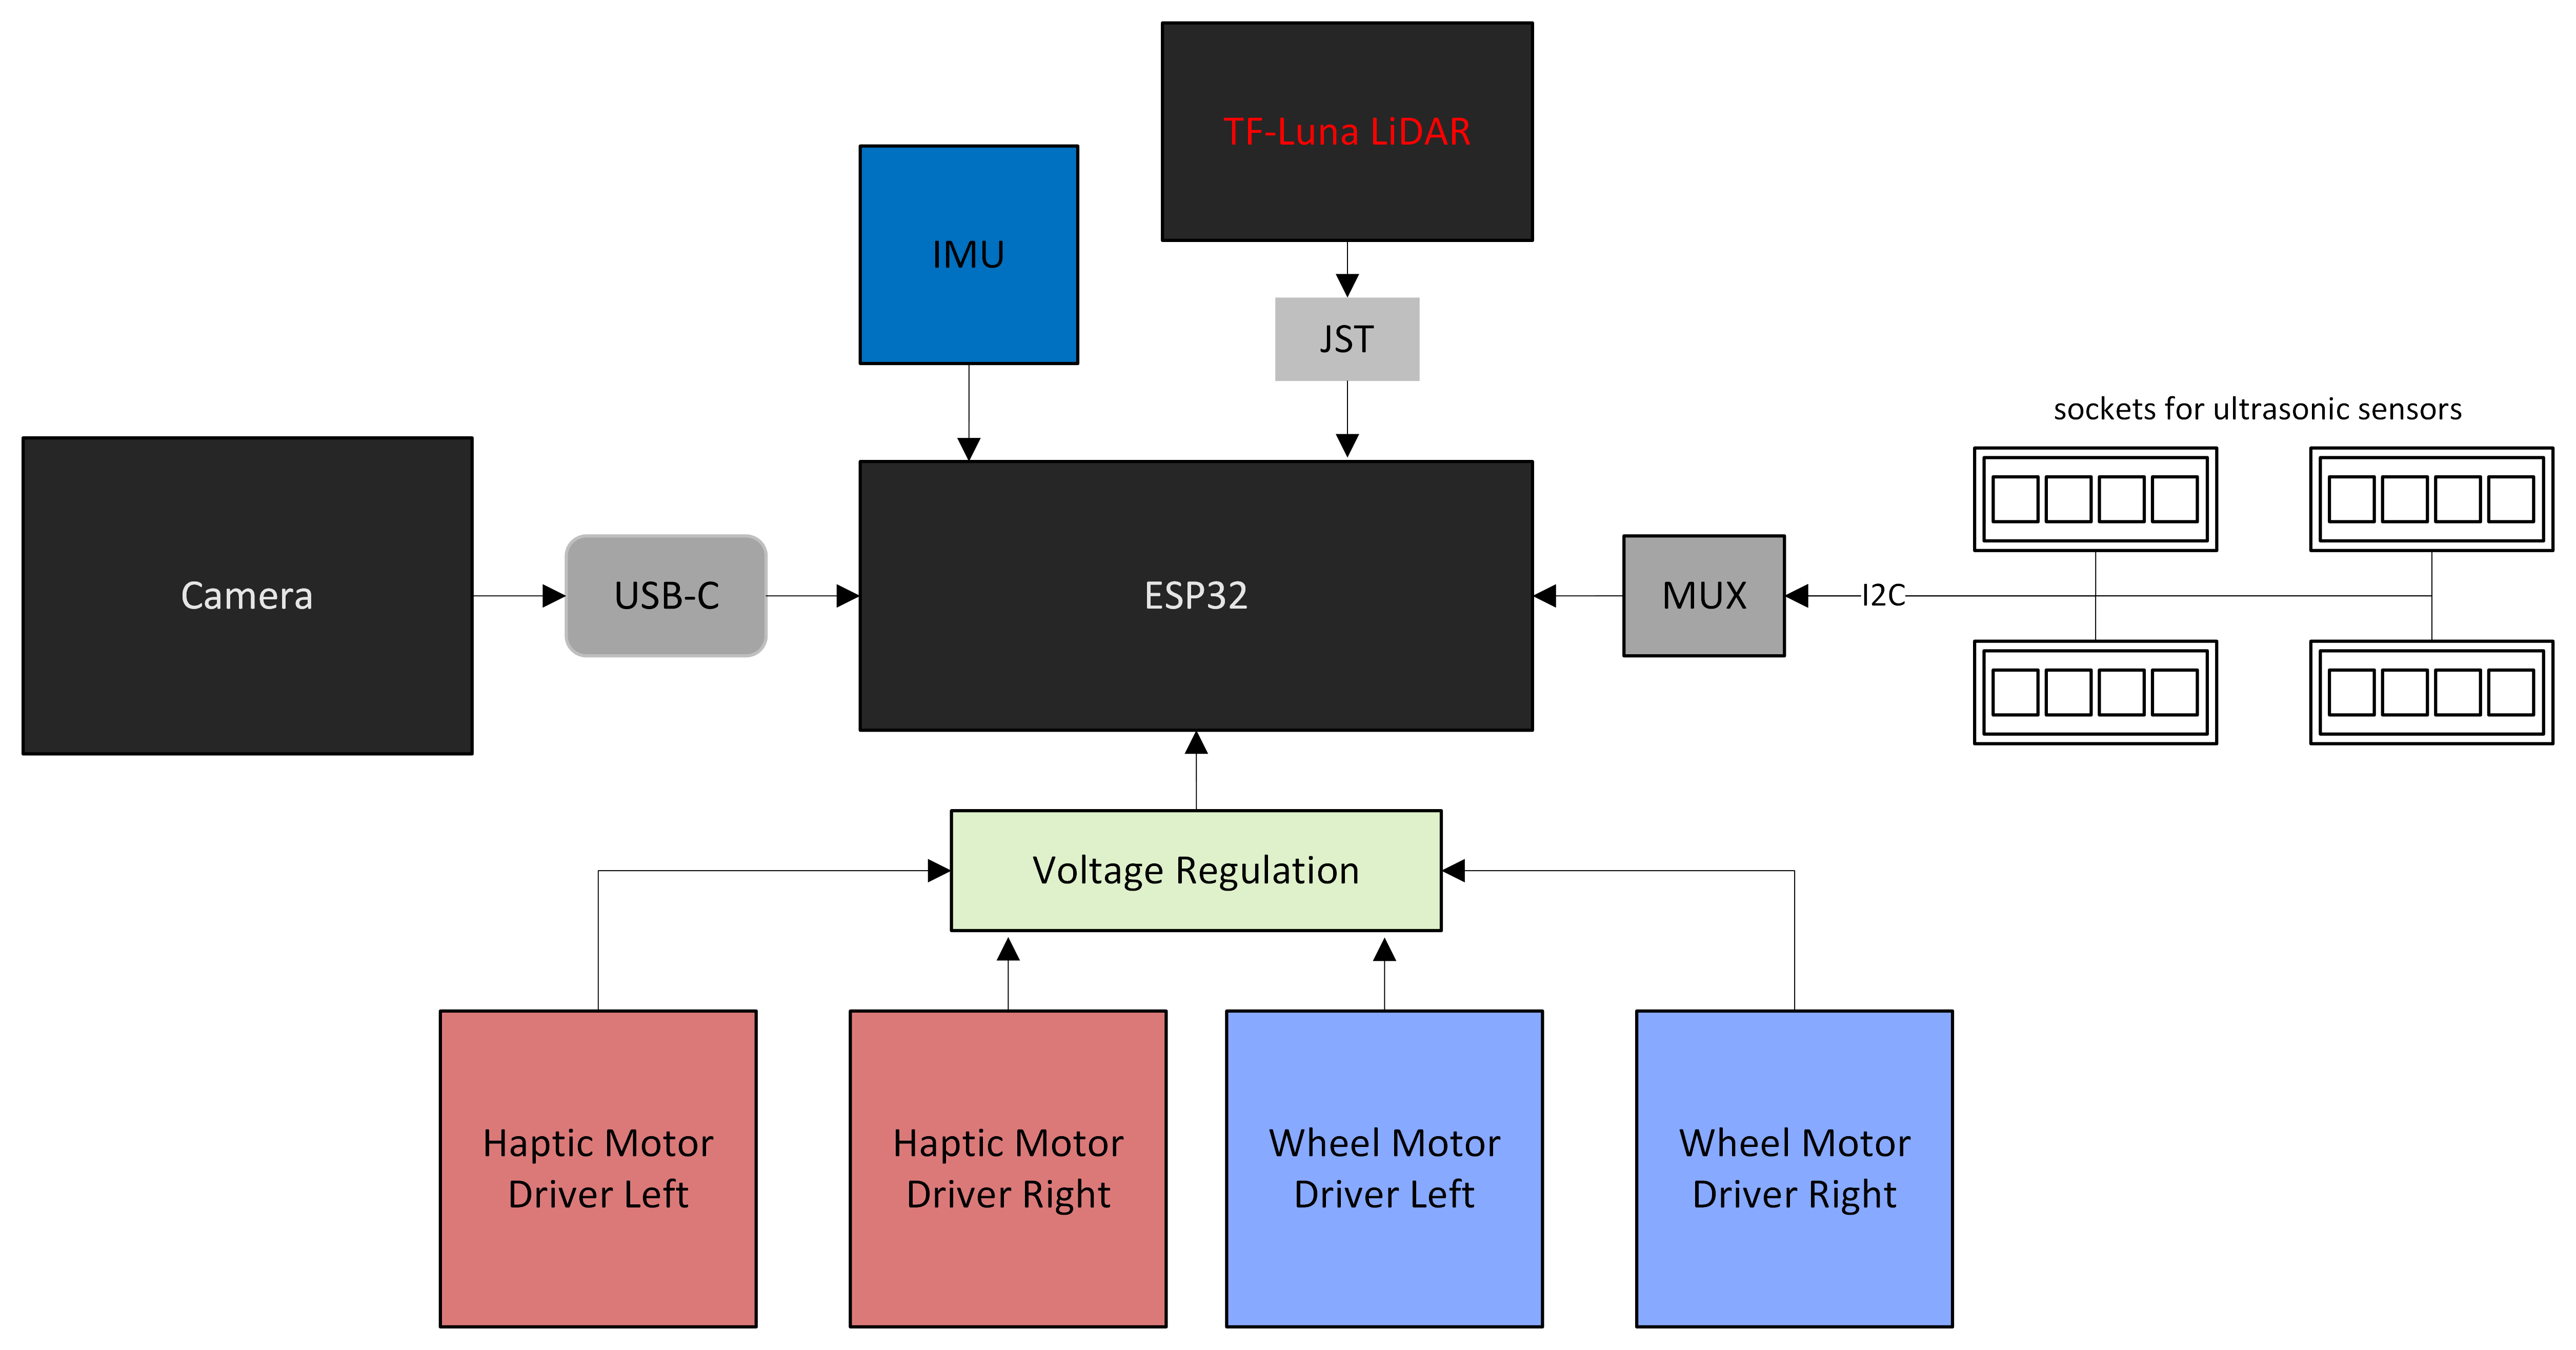
\includegraphics[width=\textwidth]{./Images/PCB-Block-Diagram.png}
	\caption{\label{fig:pcb}PCB Block Diagram}
\end{figure}

\begin{figure}[H]
	\centering
	\includegraphics[width=\textwidth]{./Images/PCB-sch.png}
	\caption{\label{fig:pcb-sch}PCB KiCAD Schematic}
\end{figure}

\begin{figure}[H]
	\centering
	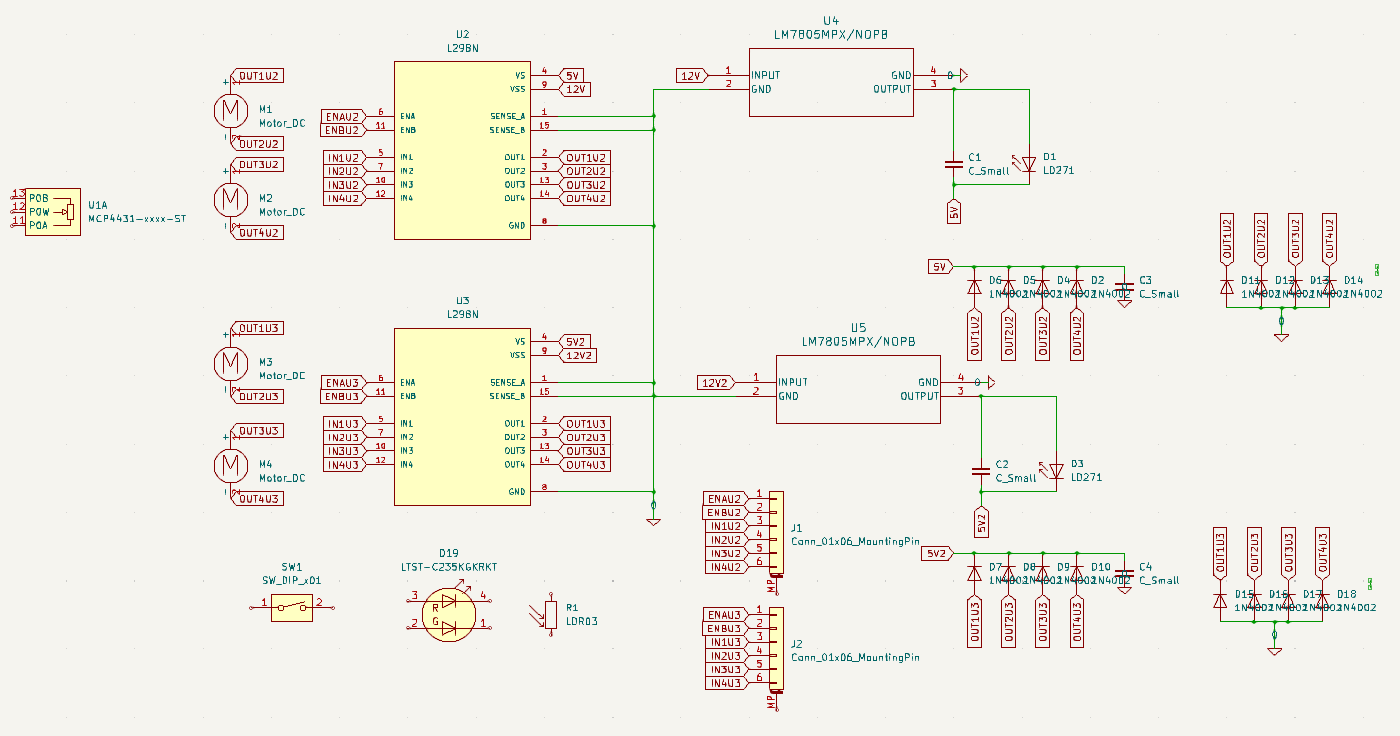
\includegraphics[width=\textwidth]{./Images/pcb-avoidance-headers.png}
	\caption{\label{fig:pcb-motor}PCB KiCAD Schematic for Avoidance Subsytem}
\end{figure}
	% PCB design philosophy, components to-be-included block diagram
	
	% 10 pages
	\newpage
	\section{System Testing}
	\subsection{Subsystem Testing}
% talks about different rigorous methods of testing the system

%\noindent FOV directivity test for range sensors, depression angle test, incoming data stream test.\\
% raise alerts if range threshold is crossed
% object detection test - range updates continuously and raises flag or interrupt if crosses below a threshold of danger
% - passing obstacle (confirm margin of safety)
% - moving obstacle
\subsubsection{Detection FOV Threshold} \label{ardumatlab}
\noindent The first test for the obstacle detection subsystem is straightforward. It will consist of the sensor readings code uploaded to the microcontroller, connected to a laptop which rests on the seat of the rollator. The serial plotter will be open and we aim to observe changes to pitch and yaw angles as well as sensor ranges all simultaneously. This will provide a visual indication and verification that the proper decisions based on detections can be created in the Senior Design II course. This test should work regardless of surface material and orientation of the obstacle. Therefore, it will be tested indoors in a hallway and open forum environment, outdoors in a neighborhood. The indoor test environments resemble that which FORWARD might be deployed in the medical hospital or assisted living facility, while it may also be driven around in lower calamity settings. Regardless, we will verify that ranging is independent of the environment.\\

\noindent Sensors must be integrated on the Medline rollator in their assigned positions, continuously transmitting the data to the microcontroller. The secondary goal will be to then connect the Arduino COM port to Matlab in order to generate a polar plot showcasing the field of vision of the rollator when outfitted with purely the range sensors. The three tiers of requirements for passing the test are as follows:
\begin{enumerate}
	\item \textbf{Basic:} Successfully detect face-on obstacles at $0.500$, $2.000$, $7.000$ meters. Range decreases and increases as the rollator is driven by the user.
	\item \textbf{Stretch:} Successfully detect obstacles at distance, at angles $\pm 15$, $\pm 30$, $\pm 90$ and sub-intervals depending on rollator attitude (degrees). Instantaneous delta in range measurement is observed when obstacle passes out of $S_x$ field of view
	\item \textbf{Advanced:} Alert the network "surrounded" or "hallway dead end" if all sensor ranges are below the 0.5 meter threshold.
\end{enumerate}
where a detection is defined by an instantaneous delta in the sensor readings, resulting in a less-than-maximum range. The distances are defined by radial distance from the center of mass of the rollator. The angles are defined in a polar manner, where the origin is also the center of mass. The coordinates $(x,y)$ of an obstacle $X_x$, detected by sensor $x$ at range $S_x$ and angle $\theta$ whose positive increase is counterclockwise in this frame is then given by:
$$X_x = S_x(cos(\theta), sin(\theta)) = (x,y)$$ \label{Polar}

\noindent As known, there are minor dead zones in the range sensors. Therefore, to determine a safe zone range threshold, it would need to exceed the range of dead sensing. Now, there could be a way to determine that FORWARD is reading the dead zone and coordinate emergency stops based on that (although it is also important to note that an emergency stop for low range may only be necessary if S2 and S3 front-facing are dead). The detection threshold can then be hard-coded into the GNC software, say $0.25$ meters.\\

\begin{figure}[H]
	\centering
	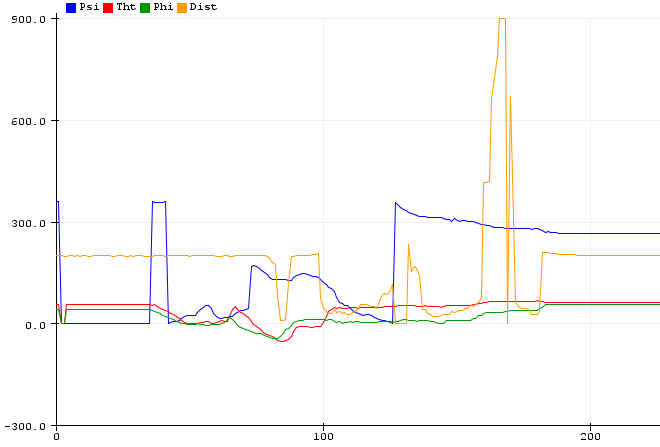
\includegraphics[width=0.7\textwidth]{./Images/serial-plotter.png}
	\caption{\label{fig:euler-test}Euler Angles Test}
\end{figure}

%\begin{figure}[H]
%	\centering
%	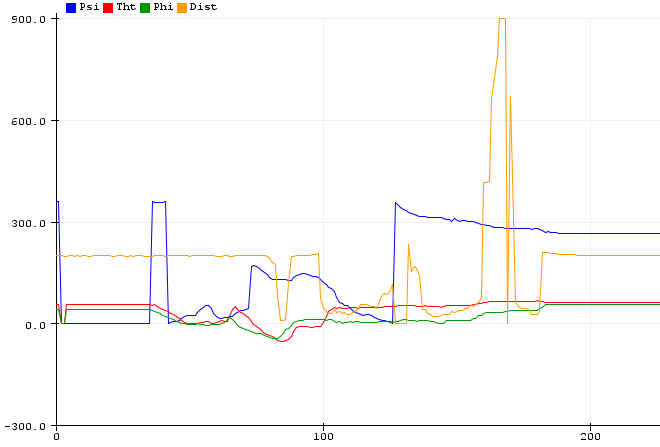
\includegraphics[width=0.7\textwidth]{./Images/serial-plotter.png}
%	\caption{\label{fig:range-test}Sensor Ranging Test}
%\end{figure}

\noindent It follows then, that we can define a range grid in polar coordinates where the maximum range detected is plotted versus yaw angle of the rollator. In this plot, we can also see precisely when there is an obstacle that causes a reduction in range.\\

% object identification test - classify obstacles and send walker into a moded resposne
% relay audio feedback to user informing them what is ahead
\subsubsection{Identification Importance}
The tiers of testing goals are:
\begin{enumerate}
	\item \textbf{Basic:} Alert the network there is a certain type of obstacle present (i.e. person, dog, car).
	\item \textbf{Stretch:} Alert the network that if two or more cars are present, "road ahead." If two or more people are present, "crowd ahead." Rank how urgent the situation is.
	\item \textbf{Advanced:} If range sensors return low but no obstacles classified, alert the network "wall." This is a placeholder code for any static solid obstacle.
\end{enumerate}

% object avoidance test - activate feedback and update motor speeds
\subsubsection{Control Feedback}
\noindent We must likewise test the haptic motors to determine if they are operational. The most important goal for this evaluation is to ensure that the components purchased are not defective, the wiring is correct, and that the programming also is correct. There are a number of issues that could arise within these processes, so simply spinning the motors would be a victory for this test. However, we will be more prepared for Senior Design II if we are able to incorporate the programming controlling the haptic motors with the rest of the code. This would involve the motors altering their vibration as a result of the sensor data and/or identifying the location of the obstacle as either on the left or right. We will zip tie the motors to the handlebars and then test the haptic feedback in a similar way as we will test the sensors. The rollator will be walked down a hallway and turned to face the wall, thus providing a difference in sensor readings. Ideally, the motors will vibrate in response to a change in distance from the ultrasonic sensors. A successful control feedback test is defined by:

\begin{enumerate}
	\item \textbf{Basic:} Successfully vibrate the rollator handlebars via the haptic motors attached.
	\item \textbf{Stretch:} Increase the frequency of vibration as range reading decreases.
	\item \textbf{Advanced:} Spatially aware haptic feedback - left and right handlebars indicate the location of the obstacle.
\end{enumerate}

 
 \noindent In addition to vibration, we will include serial print statements within the software so that we can easily troubleshoot incorrect behavior from the haptics. If the statement printed in serial is not corresponding to the actions of the motors, we know that there is a hardware issue, either with the MCU, motors, or wiring. Contrarily, if the expected statement is not printed in the serial monitor, we can reasonably assume that there is a software issue.\\

% in SD2, will need to refine turning ratios, hazard range thresholds, and work on stretch requirements.
\subsection{System Integration, Testing, and Evaluation}
\noindent System integration was already incorporated to some extent into the subsystem testing described in the previous subsection. However, there will be further concerns and scrutiny the FORWARD system must be subjected to as a whole. Among basic properties such as secure mounting and housing in the electronics chassis (discussed in section \ref{chassis}), it is good to consider waterproofing, temperature, viability with low battery/power supply, and configurations with sensors on, camera off, or vice versa. This should be done in order to ensure a reliable product is brought to the user.\\

\noindent \underline{\textit{PCB Assembly and Testing}}
\noindent As mentioned, the printed circuit board should be tested with varying levels of battery life remaining. It is likely that we will need to order a new PCB after testing our initial PCB as it is common for there to be issues such as changes in components, missed voltage regulation requirements, broken connections, incorrect sizing, lack of electrical isolation, or miswiring. Of course we will attempt to prepare for these mishaps, yet there is still a necessity  for testing and evaluation.\\

\noindent \underline{\textit{Determining and tuning motor coefficients}} During integration, it will be necessary to assign values governing the yaw steering command to the speed of the motors and haptic feedback signals. There should exist some constants that taking into account the rollator dynamics, can be calculated to scale the motors in order to achieve the desired turning angle. Additionally, once integration has been achieved, these scalars can be fine-tuned to optimize the rollator performance response.\\

\noindent \underline{\textit{Autonomous Navigation with Cooperative User}}
\noindent With motors installed on the rollator, which is also equipped with GNC software, there should be decision-making in the main code to distinguish how FORWARD adapts based on the environment. Some scenarios that come to mind are:
\begin{enumerate}
	\item Evasive mode. FORWARD takes full control (i.e. emergency stop)
	\item Cooperative navigation mode. FORWARD guides the user in a way does not infringe on their free movement.
	\item Dormant mode. User has full control of direction. \footnote{This is distinct from system powered off because the electronics are still in operation, they are just not being stimulated from the environment in a way that demands response from FORWARD}
\end{enumerate}
This step is probably the most difficult to implement at the same time as PCB development, motor coefficient tuning, and critical design review are taking place. Oftentimes, system moding is not as straightforward as it is cut out to be; in the boundary conditions when FORWARD will transition from one mode to the next, the team will have to carefully design the GNC software to remain stable. In other words, it remains subjective exactly when to apply emergency braking or how to define edge cases of multi-obstacle scenarios. Curb lifting, headlights in lowlight environments, and the other advanced requirements also remain undefined at this time.\\

\noindent \underline{\textit{Free Roam Evaluation}}
\noindent The final phase of testing is done when FORWARD integration is complete, and this is called the free roam evaluation. Essentially, the walker will be driven out in public for a pre-determined period of time, and the team will note mishaps and incidents that the guidance, navigation, and control protocols fail to prevent. These would be noted for future improvements for future endeavors and projects or products. This evaluation method will truly test and determine the successful or unsuccessful implementation of FORWARD from the beginning specifications and requirements listed. Multi-obstacle scenarios, mixtures of incline and decline territories, and mild levels of danger will be encountered. If requirements are met, design is up to specification, and all previous tests have been passed, we are confident FORWARD evaluation will be a success.\\
	
	% 5 pages
	\newpage
	\section{Administrative Content}
	\subsection{Project Milestones}
\noindent The figure below shows various project milestones with their estimated start and end dates. The duration is given in days. There is also a Gantt chart generated by this data. The paper should be incrementally completed throughout the first semester, progressing towards a subsystem demo before an official full system prototype is made on a breadboard. After that is done, the printed circuit board will be ordered and the entirety of the second semester will be dedicated to integration and final testing and assembly. \\

\begin{figure}[H]
	\centering
	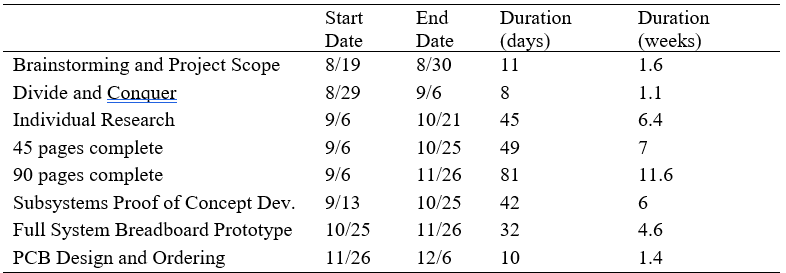
\includegraphics[width=\textwidth]{./Images/SD1mile.png}
	\caption{\label{fig:SD1mile}Senior Design I Milestones}
\end{figure}

\begin{figure}[H]
	\centering
	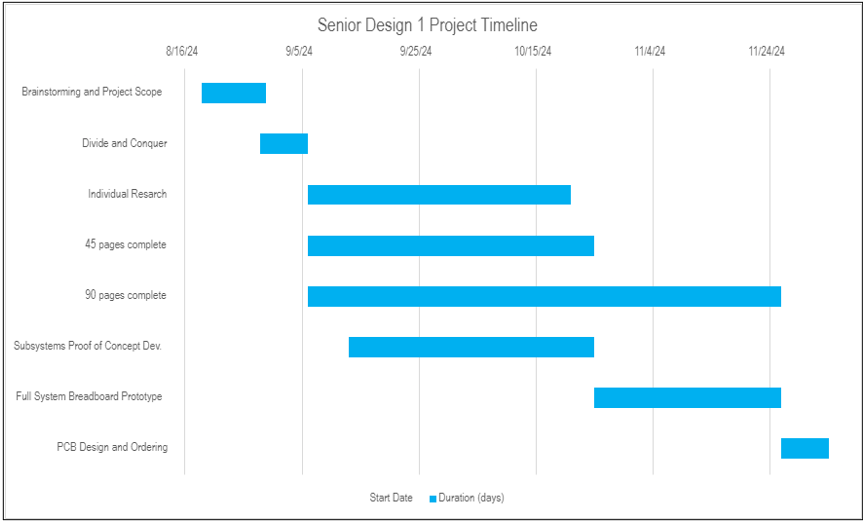
\includegraphics[width=\textwidth]{./Images/SD1gantt.png}
	\caption{\label{fig:SD1gantt}Senior Design I Gantt Chart}
\end{figure}

\begin{figure}[H]
	\centering
	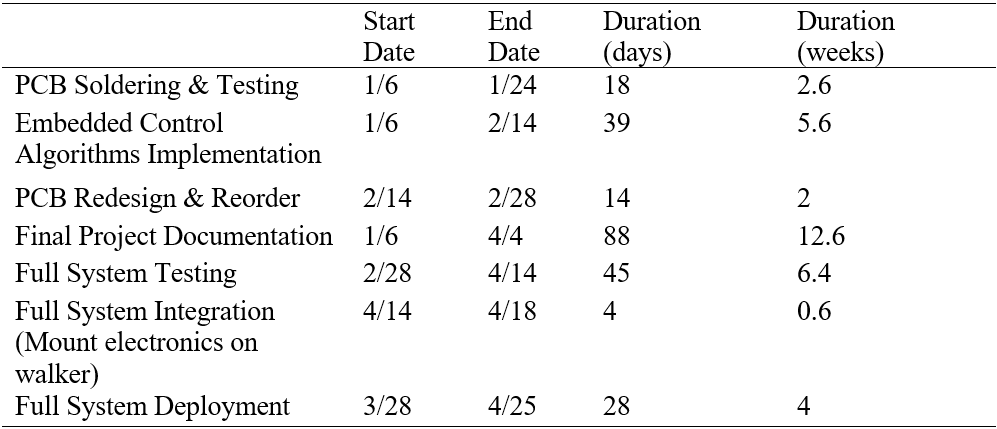
\includegraphics[width=\textwidth]{./Images/SD2mile.png}
	\caption{\label{fig:SD2mile}Senior Design II Milestones}
\end{figure}

\begin{figure}[H]
	\centering
	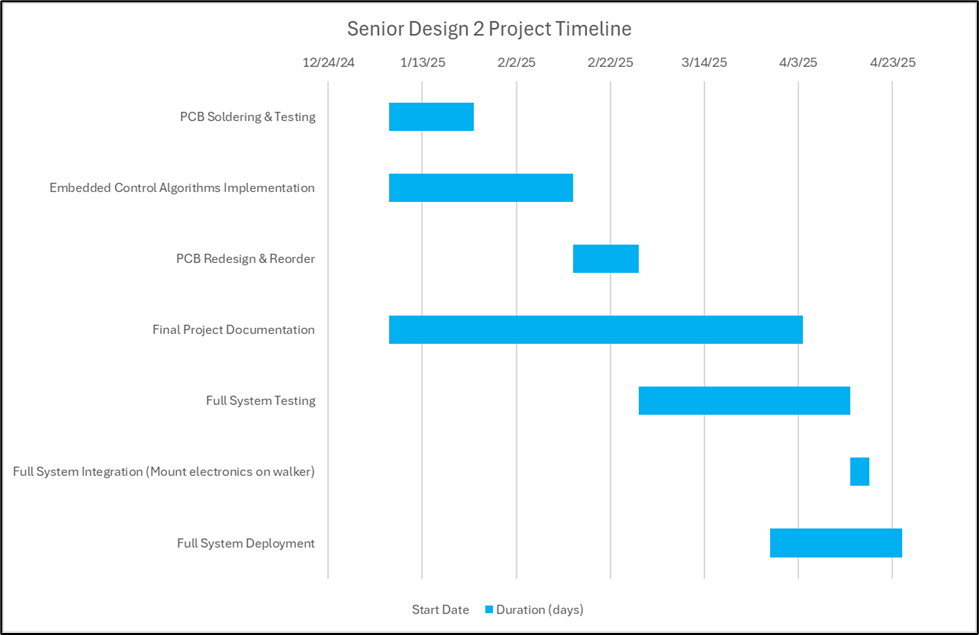
\includegraphics[width=\textwidth]{./Images/SD2gantt.png}
	\caption{\label{fig:SD2gantt}Senior Design II Gantt Chart}
\end{figure}
	\subsection{Project Budget} \label{sec:budget}
\noindent The table above shows the budget for FORWARD. As we continue to research and develop, there will likely be changes made to this table. The project will require a pre-built walker as well as 5 peripheral components, 2 motors, and 2 controllers, as well as wiring and PCB housing. \\

\begin{figure}[H]
	\centering
	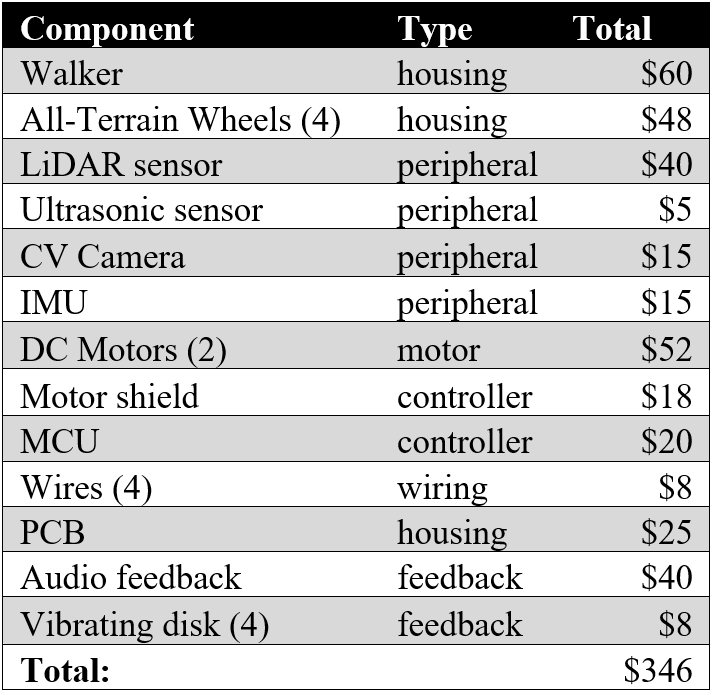
\includegraphics[width=0.5\textwidth]{./Images/Budget.png}
	\caption{\label{fig:Budget}Project Budget}
\end{figure}

\subsection{Project Bill of Materials} \label{sec:BOM}
\noindent Up to this point, the budget for sensors, processors, and motors has been successfully upheld. As advised by Dr. Wei early on to search Craig's List for a rollator, so we did and have found a great deal by a local close to UCF! Below are the expenditures to this point. We have yet to order PCB's at the time of submitting this document. Integration costs will inevitably come in senior design II.

\begin{figure}[H]
	\centering
	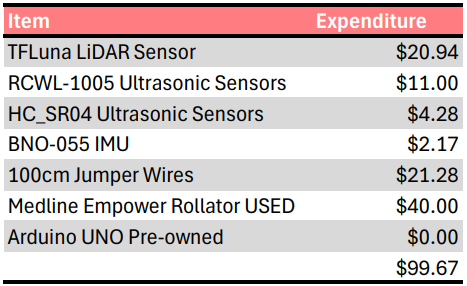
\includegraphics[width=0.5\textwidth]{./Images/detect-bom.png}
	\caption{\label{fig:detect-bom}Detection Subsystem Expenditures}
\end{figure}

\begin{figure}[H]
	\centering
	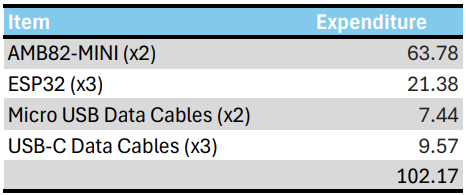
\includegraphics[width=0.5\textwidth]{./Images/identify-bom.png}
	\caption{\label{fig:identify-bom}Identification Subsystem Expenditures}
\end{figure}

\begin{figure}[H]
	\centering
	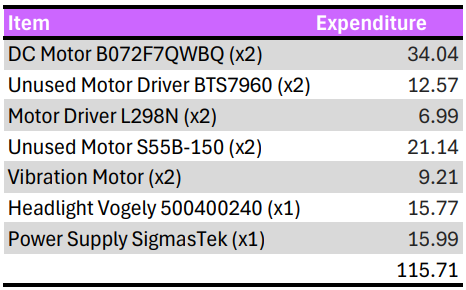
\includegraphics[width=0.5\textwidth]{./Images/avoid-bom.png}
	\caption{\label{fig:avoid-bom}Avoidance Subsystem Expenditures}
\end{figure}
		
	% 1 pages
	\newpage
	\section{Conclusion}
	
	% not included in page count
	\newpage
	\pagenumbering{roman}
	\section{Appendix A - Permissions}
	
\begin{center}
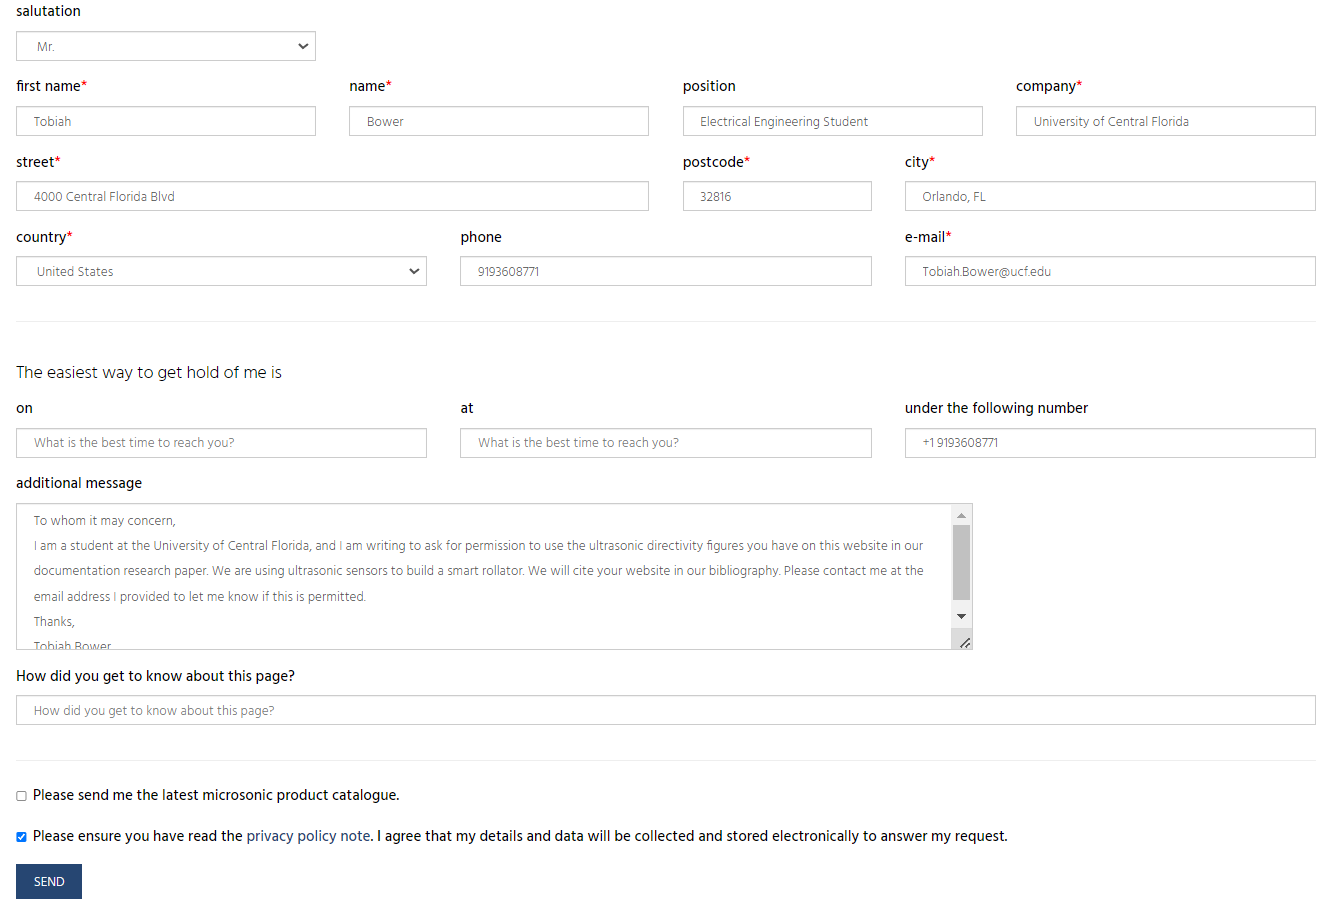
\includegraphics[width=\textwidth]{./Images/permit1.png}
\newline Request for Ultrasonic Directivity from Microsonic\\

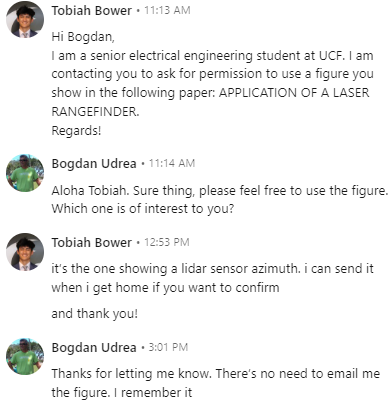
\includegraphics[width=\textwidth]{./Images/permit2.png}
\newline Request for LiDAR Azimuth from Bogdan Udrea\\

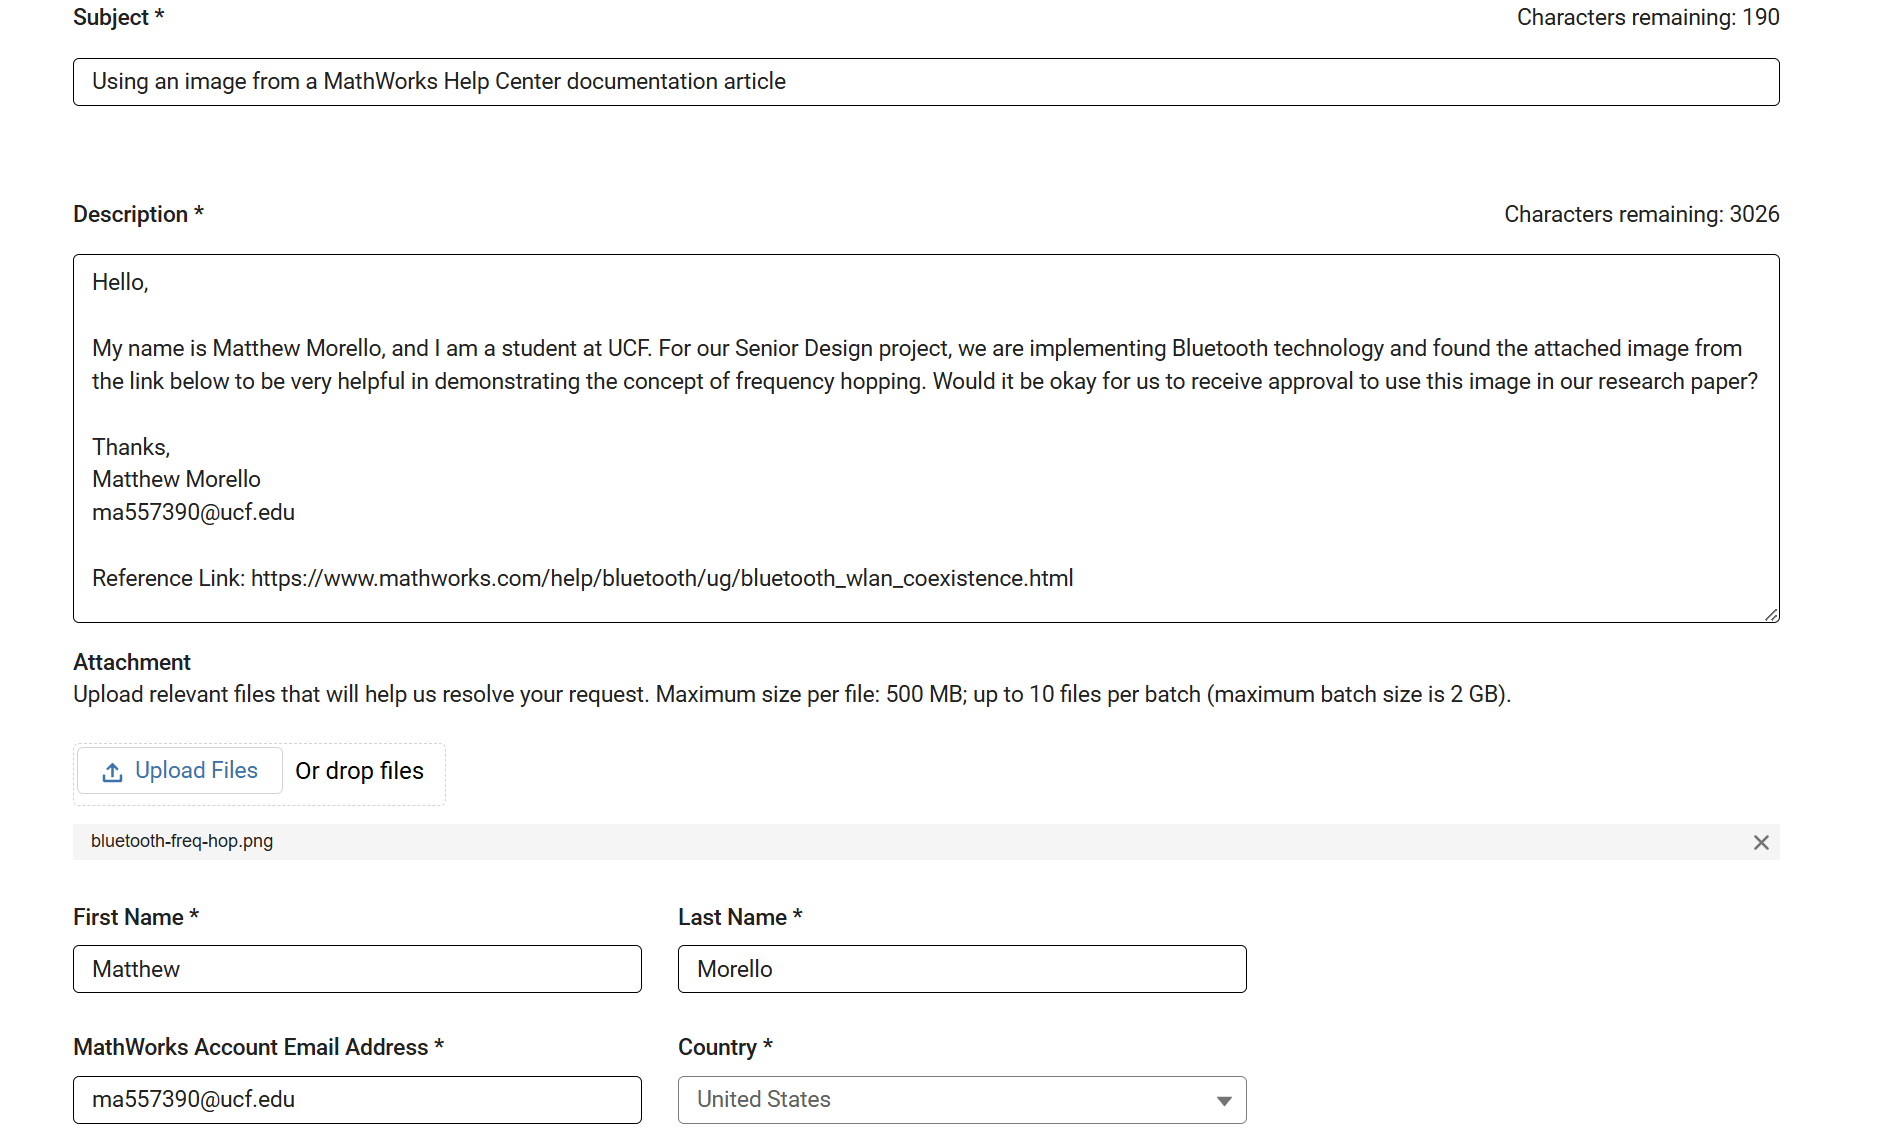
\includegraphics[width=\textwidth]{./Images/BT_Image_Use_MW.png}
\newline Request for Bluetooth Frequency Hopping from MathWorks\\

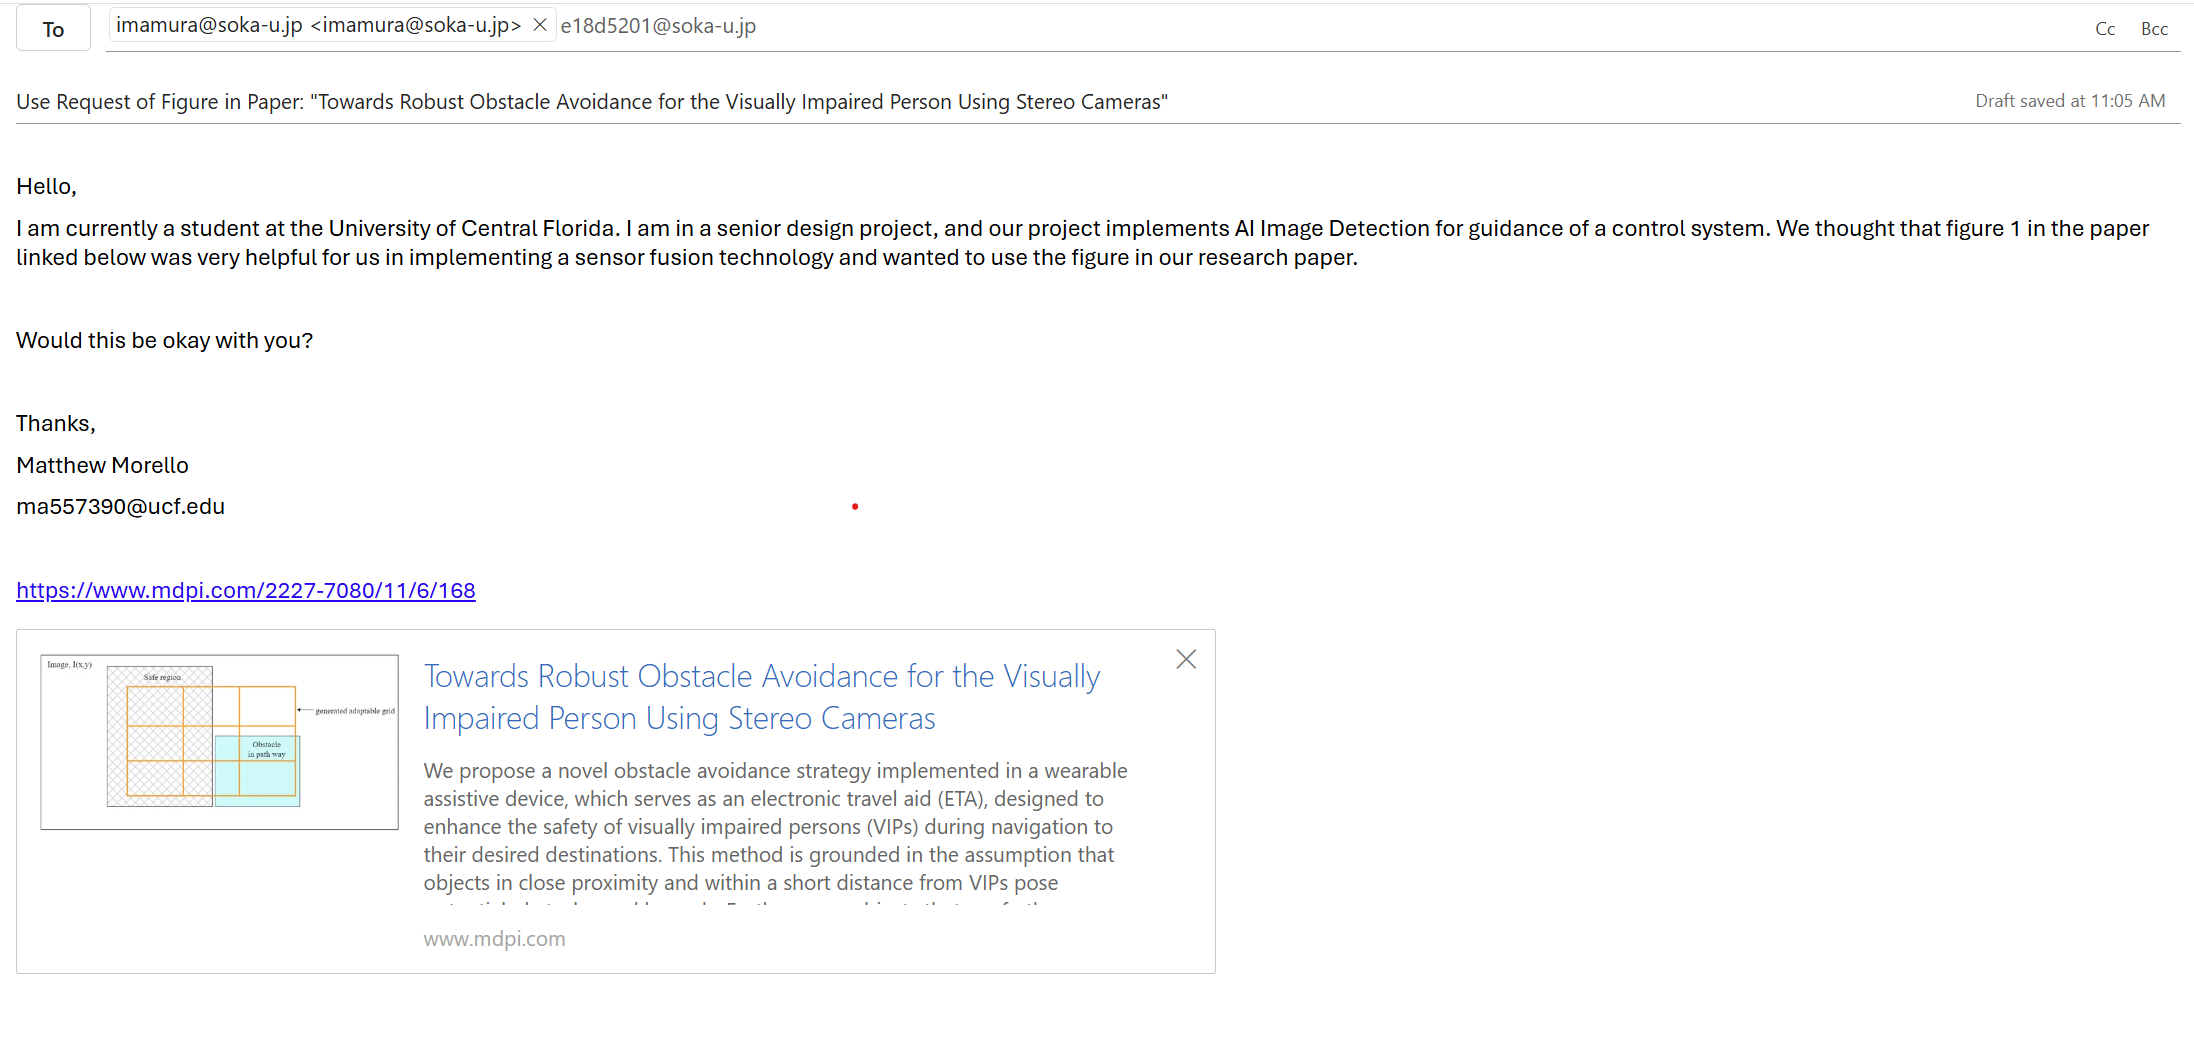
\includegraphics[width=\textwidth]{./Images/Grid_Image_Perm.png}
\newline Request for Bluetooth Frequency Hopping from MathWorks\\
\end{center}
	
	\newpage
	\section{Appendix B - References}
	\begin{thebibliography}{45}
	
	% seminal UCF work
	\bibitem{Mostofa} Mostofa N, Feltner C, Fullin K, Guilbe J, Zehtabian S, Bacanlı SS, Bölöni L, Turgut D. A Smart Walker for People with Both Visual and Mobility Impairment. Sensors. 2021; 21(10):3488. \href{https://doi.org/10.3390/s21103488}{https://doi.org/10.3390/s21103488}
	
	% seminal work all-time
	\bibitem{PAMM} S. Dubowsky et al., "PAMM - a robotic aid to the elderly for mobility assistance and monitoring: a 'helping-hand' for the elderly," Proceedings 2000 ICRA. Millennium Conference. IEEE International Conference on Robotics and Automation. Symposia Proceedings (Cat. No.00CH37065), San Francisco, CA, USA, 2000, pp. 570-576 vol.1, \href{https://doi.org/10.1109/ROBOT.2000.844114}{doi:10.1109/ROBOT.2000.844114}
	
	% object detection AI/ML GNC application paper for VIPs
	\bibitem{CVRef1} B. K. Asiedu Asante and H. Imamura, "Towards Robust Obstacle Avoidance for the Visually Impaired Person Using Stereo Cameras," Technologies, vol. 11, no. 6, p. 168, 2023. \href{https://doi.org/10.3390/technologies11060168}{doi:10.3390/technologies11060168}
	
	% Lightweight model focused project
	\bibitem{CVRef2} A. B. Atitallah, Y. Said, M. A. B. Atitallah, M. Albekairi, K. Kaaniche, and S. Boubaker, "An effective obstacle detection system using deep learning advantages to aid blind and visually impaired navigation," Ain Shams Engineering Journal, vol. 15, no. 2, p. 102387, 2024. \href{https://doi.org/10.1016/j.asej.2023.102387}{doi:10.1016/j.asej.2023.102387}
	
	% ESP32 BLE environmental sensing project example
	\bibitem{bluetoothSensorProject} Rui Santos, "ESP32 BLE Server – Environmental Sensing Service (ESP-IDF)," Random Nerd Tutorials, 6 October 2022. [Online]. Available: \href{https://randomnerdtutorials.com/esp32-ble-server-environmental-sensing-service/}{https://randomnerdtutorials.com/esp32-ble-server-environmental-sensing-service/}. [Accessed: Oct. 29, 2024].

	% ESP32 camera module project ref
	\bibitem{ESP32CamRef1} How2Electronics, "ESP32-CAM based object detection \& identification with OpenCV," How2Electronics. [Online]. Available: \href{https://how2electronics.com/esp32-cam-based-object-detection-identification-with-opencv/}{https://how2electronics.com/esp32-cam-based-object-detection-identification-with-opencv/}. [Accessed: Oct. 9, 2024].
	
	% RealTek Camera Project Ref
	\bibitem{RealTekCamRef1} How To Electronics, "Object Detection \& Identification with AMB82 Mini AI Camera," How2Electronics. Available: \href{https://how2electronics.com/object-detection-identification-with-amb82-mini-ai-camera/}{https://how2electronics.com/object-detection-identification-with-amb82-mini-ai-camera/}. [Accessed: Oct. 9, 2024].
	
	\bibitem{HowYOLOWorks} R. Kumar, "YOLO Object Detection Explained," DataCamp, https://www.datacamp.com/blog/yolo-object-detection-explained. (accessed Oct. 24, 2024).
	
	% Bone conduction ref article
	\bibitem{BoneConductionRef} Soundscape HQ, "Unlock Sound Through Bones: Understanding Bone Conduction," \emph{Soundscape HQ}, 2024. [Online]. Available: \href{https://soundscapehq.com/what-is-bone-conduction/}{https://soundscapehq.com/what-is-bone-conduction/}. [Accessed: Oct. 15, 2024].

	\bibitem{bluetooth} Bluetooth Technology, "Tech Overview," Bluetooth.com, https://www.bluetooth.com/learn-about-bluetooth/tech-overview/. (accessed Oct. 24, 2024).
	
	\bibitem{bluetoothHow} C. Woodford, "How Bluetooth Works," Explain That Stuff, https://www.explainthatstuff.com/howbluetoothworks.html. (accessed Oct. 24, 2024).

	% Amazon Bone Conduction Ear Pieces
	\bibitem{BoneConductEar1} YouthWhisper Bone Conduction Headphones Bluetooth, Wireless Open-Ear Headset with Microphones, Titanium Lightweight Sweat Resistant, Answer Phone Sports Earphones for Running Hiking Bicycling Black \href{https://www.walmart.com/ip/YouthWhisper-Bone-Conduction-Headphones-Bluetooth-Wireless-Open-Ear-Headset-Microphones-Titanium-Lightweight-Sweat-Resistant-Answer-Phone-Sports-Earp/278825770?clickid=WjORv5UqyxyKRJqTvVUblVgLUkCRR\%3AxQe1ri}{https://www.walmart.com/ip/YouthWhisper-Bone-Conduction-Headphones-Bluetooth-Wireless-Open-Ear-Headset-Microphones-Titanium-Lightweight-Sweat-Resistant-Answer-Phone-Sports-Earp/278825770}
	
	% Amazon ambient sound earbuds
	\bibitem{AmbientSoundEarbuds} JLab Wireless Bluetooth Charging Multipoint Earbuds, Ambient Sound Mode. \href{https://www.amazon.com/JLab-Wireless-Bluetooth-Charging-Multipoint/dp/B0CC772D37}{https://www.amazon.com/JLab-Wireless-Bluetooth-Charging-Multipoint/dp/B0CC772D37}
	
	% sensor fusion fall detection
	\bibitem{FallDetect} D. -M. Ding, Y. -G. Wang, W. Zhang and Q. Chen, "Fall Detection System on Smart Walker Based on Multisensor Data Fusion and SPRT Method," in IEEE Access, vol. 10, pp. 80932-80948, 2022. \href{https://doi.org/10.1109/ACCESS.2022.3195674}{doi:10.1109/ACCESS.2022.3195674}
	
	% lidar smart walker
	\bibitem{mstate} T. Dirheimer, J. Hancock, D. Hill, Y. Kochubievsky, and S. Moore, Smart Walker Design: Final Report, ECE 480, Michigan State University, April 29, 2015.
	
	\bibitem{lidar-type} ThinkAutonomous. “Types of LiDAR: What's the difference? | Think Autonomous,” ThinkAutonomous.ai, [Online]. Available: \href{https://www.thinkautonomous.ai/blog/types-of-lidar/}{https://www.thinkautonomous.ai/blog/types-of-lidar/}. Accessed: Sep. 15, 2024.
	
	\bibitem{sonar-type} M. Toa and A. Whitehead, "Ultrasonic Sensing Basics," Texas Instruments, Application Report SLAA907D, Dec. 2021. [Online]. Available: \href{https://www.ti.com/lit/an/slaa907d/slaa907d.pdf}{https://www.ti.com/lit/an/slaa907d/slaa907d.pdf}. Accessed: Sep. 15, 2024.
	
	% sonar vs lidar
	\bibitem{sonar-vs-lidar} "Laser vs Ultrasonic Distance Sensor Tests," DroneBot Workshop, Sep. 29, 2019. [Online]. Available: \href{https://dronebotworkshop.com/laser-vs-ultrasonic-distance-sensor-tests/}{https://dronebotworkshop.com/laser-vs-ultrasonic-distance-sensor-tests/}. [Accessed: Sep. 10, 2024].
	
	% camera vs. lidar/ultrasonic
	\bibitem{camera-vs-sensor} "Pros and cons of camera, LiDAR, RADAR, and ultrasonic detection technologies in AV," \textit{ResearchGate}. [Online]. Available: \href{https://www.researchgate.net/figure/Pros-and-cons-of-camera-LiDAR-RADAR-and-ultrasonic-detection-technologies-in-AV\_tbl}{https://www.researchgate.net/figure/Pros-and-cons-of-camera-LiDAR-RADAR-and-ultrasonic-detection-technologies-in-AV\_tbl}. [Accessed: Sep. 15, 2024].
	
	% ultrasonic directivity figure
	\bibitem{coolUltraDirect} Microsonic, "Detection Zones," Microsonic, [Online]. Available: \href{https://www.microsonic.de/en/support/ultrasonic-technology/detection-zones.htm}{https://www.microsonic.de/en/support/ultrasonic-technology/detection-zones.htm}. [Accessed: 15-Sep-2024].
	
	% lidar FOV figure
	\bibitem{coolLiDARfov} R. M. [Last Name], "FOV Definition: Optical axis of scanning LIDAR (Black dotted line)," ResearchGate, [Online]. Available: \href{https://www.researchgate.net/figure/FOV-Definition-Optical-axis-of-scanning-LIDAR-Black-dotted-line\_fig1\_280132809}{https://www.researchgate.net/figure/FOV-Definition-Optical-axis-of-scanning-LIDAR-Black-dotted-line\_fig1\_280132809}. [Accessed: 15-Sep-2024].
	
	% walker with stretch requirements: stability and curb lifter
	\bibitem{byACRE} byACRE, "Carbon Ultralight Rollator," byACRE, [Online]. Available: \href{https://shop.byacre.com/us/carbon-ultralight-rollator.html}{https://shop.byacre.com/us/carbon-ultralight-rollator.html}. [Accessed: 16-Sep-2024].
	
	% walker with mechanical speed control (not electronic) and curb lifting
	\bibitem{ustep} uStep, "Standard Model," uStep, Available: \href{https://www.ustep.com/product/standard-model}{https://www.ustep.com/product/standard-model}.
	
	% quaternions
	\bibitem{quat} E. W. Weisstein, "Quaternion," MathWorld--A Wolfram Web Resource. [Online]. Available: \href{https://mathworld.wolfram.com/Quaternion.html.}{https://mathworld.wolfram.com/Quaternion.html.}.
	
	% seminal Kalman filter paper
	\bibitem{kalman} R. E. Kalman, "A new approach to linear filtering and prediction problems," Journal of Basic Engineering, vol. 82, no. 1, pp. 35-45, Mar. 1960. [Online]. Available: \href{https://www.cs.unc.edu/~welch/kalman/media/pdf/Kalman1960.pdf}{https://www.cs.unc.edu/~welch/kalman/media/pdf/Kalman1960.pdf}.
	
	% how brakes work
	\bibitem{Brain} Brain, M. (n.d.). How brakes work. HowStuffWorks. \href{https://auto.howstuffworks.com/auto-parts/brakes/brake-types/brake.htm}{https://auto.howstuffworks.com/auto-parts/brakes/brake-types/brake.htm}
	
	% finding how long a battery will last - calculator
	\bibitem{Calculator Academy} Calculator Academy. (n.d.). Battery run time calculator. Calculator Academy. \href{https://calculator.academy/battery-run-time-calculator/}{https://calculator.academy/battery-run-time-calculator/}
	
	% market analysis
	\bibitem{Grand View Research} Grand View Research. (2024). Assisted walking devices market size, share \& trends analysis report by product type (Canes, Crutches, Walkers, Gait Trainers), by region, and segment forecasts, 2022 - 2030. Grand View Research. \href{https://www.grandviewresearch.com/industry-analysis/assisted-walking-device-market}{https://www.grandviewresearch.com/industry-analysis/assisted-walking-device-market}
	
	% what bicycle lights are required by law
	\bibitem{Perez} Mallard Perez. (n.d.). What the Florida law says about bicycle lights. Mallard Perez. \href{https://www.mallardperez.com/faqs/what-the-florida-law-says-about-bicycle-lights.cfm}{https://www.mallardperez.com/faqs/what-the-florida-law-says-about-bicycle-lights.cfm}.
	
	\bibitem{apollo} Apollo Scooters, "Understanding Electric Scooter Controllers," Apollo Scooters, [Online]. Available: \href{https://apolloscooters.co/blogs/news/understanding-electric-scooter-controllers?srsltid=AfmBOoqWTbV4qa2VxA8NxpdquVzQMn4LeQYiwBG756xhscX0vExgNW-8}{https://apolloscooters.co/blogs/news/understanding-electric-scooter-controllers}. [Accessed: Oct. 24, 2024].
	
	\bibitem{hwang2020} J. S. Hwang, S. Y. Kim, and H. M. Kim, "A Study on the Design of the Control Algorithm for the Electric Scooter," \textit{IEEE Access}, vol. 8, pp. 146207-146215, 2020. \href{https://ieeexplore.ieee.org/document/9137951}{https://ieeexplore.ieee.org/document/9137951}. [Accessed: Oct. 24, 2024].

	\bibitem{coreelectronics} Core Electronics, "Motor Drivers vs. Motor Controllers," Core Electronics, [Online]. Available: \href{https://core-electronics.com.au/guides/motor-drivers-vs-motor-controllers/}{https://core-electronics.com.au/guides/motor-drivers-vs-motor-controllers/}. [Accessed: Oct. 24, 2024].
	
	\bibitem{thingbits} Thingbits, "Motor Drivers," Thingbits, [Online]. Available: \href{https://www.thingbits.in/t/categories/motors-and-drivers/motor-drivers}{https://www.thingbits.in/t/categories/motors-and-drivers/motor-drivers}. [Accessed: Oct. 24, 2024].
	
	\bibitem{powerelectronics} Power Electronics News, "Learning the Basics of Motor Control," Power Electronics News, [Online]. Available: \href{https://www.powerelectronicsnews.com/learning-the-basics-of-motor-control/}{https://www.powerelectronicsnews.com/learning-the-basics-of-motor-control/}. [Accessed: Oct. 24, 2024].
	
	\bibitem{etechsparks} Etech Sparks, "DC Motor Controller: Working Principle \& Definition," Etech Sparks, [Online]. Available: \href{https://etechsparks.com/dc-motor-controller-working-principle-definition/}{https://etechsparks.com/dc-motor-controller-working-principle-definition/}. [Accessed: Oct. 24, 2024].
	
	\bibitem{elprocus1} Elprocus, "Different Types of Electric Motors," Elprocus, [Online]. Available: \url{https://www.elprocus.com/different-types-of-electric-motors/}. [Accessed: Oct. 24, 2024]. 
	
	\bibitem{pihut} The Pi Hut, "What's the Difference Between DC, Servo \& Stepper Motors?" The Pi Hut, [Online]. Available: \url{https://thepihut.com/blogs/raspberry-pi-tutorials/whats-the-difference-between-dc-servo-amp-stepper-motors}. [Accessed: Oct. 24, 2024]. 
	
	\bibitem{powerelectric} Power Electric, "AC Motors vs. DC Motors," Power Electric, [Online]. Available: \url{https://www.powerelectric.com/motor-blog/ac-motors-vs-dc-motors}. [Accessed: Oct. 24, 2024]. 
	
	\bibitem{elprocus2} Elprocus, "DC Motor: Basics, Types, and Applications," Elprocus, [Online]. Available: \url{https://www.elprocus.com/dc-motor-basics-types-application/}. [Accessed: Oct. 24, 2024]. 
	
	\bibitem{elprocus3} Elprocus, "DC Shunt Motor: Construction, Working Principle, and Circuit Diagram," Elprocus, [Online]. Available: \url{https://www.elprocus.com/dc-shunt-motor-construction-working-principle-circuit-diagram/}. [Accessed: Oct. 24, 2024]. 
	
	\bibitem{elprocus4} Elprocus, "DC Series Motor: Components, Circuit Diagram, and Applications," Elprocus, [Online]. Available: \url{https://www.elprocus.com/dc-series-motor-components-circuit-diagram-applications/}. [Accessed: Oct. 24, 2024]. 
	
	\bibitem{elprocus5} Elprocus, "PMDC (Permanent Magnetic DC) Motor: Construction and Working," Elprocus, [Online]. Available: \url{https://www.elprocus.com/pmdc-permanent-magnetic-dc-motor-construction-working/}. [Accessed: Oct. 24, 2024]. 
	
	\bibitem{linquip} Linquip, "Compound DC Motors," Linquip, [Online]. Available: \url{https://www.linquip.com/blog/compound-dc-motors/}. [Accessed: Oct. 24, 2024]. 
	
	\bibitem{elprocus6} Elprocus, "Brushless DC Motor: Advantages, Applications, and Control," Elprocus, [Online]. Available: \url{https://www.elprocus.com/brushless-dc-motor-advantages-applications-and-control/}. [Accessed: Oct. 24, 2024]. 
	
	\bibitem{monolithicpower} Monolithic Power Systems, "Brushless vs. Brushed DC Motors," Monolithic Power Systems, [Online]. Available: \url{https://www.monolithicpower.com/en/learning/resources/brushless-vs-brushed-dc-motors}. [Accessed: Oct. 24, 2024].
	
	\bibitem{spikevm} 
	Spike VM, "RPM to MPH Calculator," Spike VM, [Online]. Available: \url{https://www.spikevm.com/calculators/fuel_distance/rpm-mph.php}. [Accessed: Oct. 24, 2024]. 
	
	\bibitem{lee2019} 
	J. Lee, J. Kim, and H. Kim, "A Study on the Efficiency of Electric Motors," \textit{Nat. Sci. Rep.}, vol. 9, no. 1, pp. 1-11, 2019. [Online]. Available: \url{https://www.ncbi.nlm.nih.gov/pmc/articles/PMC6353162/}. [Accessed: Oct. 24, 2024]. 
	
	\bibitem{trionic} 
	Trionic, "How Much Weight Can the Rollator Hold," Trionic, [Online]. Available: \url{https://www.trionic.us/en/knowledge/135/how-much-weight-can-the-rollator-hold}. [Accessed: Oct. 24, 2024]. 
	
	\bibitem{gribble} 
	Gribble, "Cycling Power vs. Speed Calculator," Gribble, [Online]. Available: \url{https://www.gribble.org/cycling/power_v_speed.html?units=metric&rp_wr=74.843&rp_wb=17&rp_a=0.509&rp_cd=0.63&rp_dtl=1&ep_crr=0.04&ep_rho=1.22601&ep_g=8&ep_headwind=0&p2v=200&v2p=35.41}. [Accessed: Oct. 24, 2024]. 
	
	\bibitem{drive} 
	Drive Medical, "Drive Medical Rollator with Removable Back Support," Amazon, [Online]. Available: \url{https://www.amazon.com/Drive-Medical-Rollator-Removable-Support/dp/B00NFJX0PU}. [Accessed: Oct. 24, 2024]. 
	
	\bibitem{xconvert} 
	XConvert, "Square Inches to Square Feet Converter," XConvert, [Online]. Available: \url{https://www.xconvert.com/unit-converter/square-inches-to-square-feet}. [Accessed: Oct. 24, 2024]. 
	
	\bibitem{oxwheels} 
	Ox Wheels, "Does Tyre Size Affect Car Performance?" Ox Wheels, [Online]. Available: \url{https://www.oxwheels.com.au/Does-tyre-size-affect-car-performance}. [Accessed: Oct. 24, 2024]. 
	
	\bibitem{ebikesforum} 
	E-Bikes Forum, "Does a 750 Front and a 750 Rear Add Up to 1500 Watts?" E-Bikes Forum, [Online]. Available: \url{https://ebikesforum.com/threads/does-a-750-front-and-a-750-rear-add-up-to-1500-watts.5464/}. [Accessed: Oct. 24, 2024]. 
	
	\bibitem{yzl1} 
	YZL, "150W Brushless DC Motor Replacement Cylindrical 13000-15000RPM," Amazon, [Online]. Available: \url{https://www.amazon.com/Brushless-Cylindrical-13000-15000RPM-Propulsion-Specific/dp/B09NCJ24W6}. [Accessed: Oct. 24, 2024]. 
	
	\bibitem{Citphto} 
	Citphto, "775 6000-12000RPM Electric Brushless Motor," Amazon. [Online]. Available: \url{https://www.amazon.com/Citphto-775-6000-12000RPM-Electric-Electrical/dp/B0CMXM1N94}. [Accessed: Oct. 24, 2024]. 
	
	\bibitem{AliExpress1} 
	AliExpress, "Electric Brushless Motor," AliExpress. [Online]. Available: \url{https://www.aliexpress.us/item/3256807288642417.html}. [Accessed: Oct. 24, 2024]. 
	
	\bibitem{AliExpress2} 
	AliExpress, "Brushless Motor," AliExpress. [Online]. Available: \url{https://www.aliexpress.us/item/3256804436743610.html}. [Accessed: Oct. 24, 2024]. 
	
	\bibitem{AliExpress3} 
	AliExpress, "DC Brushless Motor," AliExpress. [Online]. Available: \url{https://www.aliexpress.us/item/3256802991206296.html}. [Accessed: Oct. 24, 2024]. 
	
	\bibitem{AliExpress4} 
	AliExpress, "High Torque Brushless Motor," AliExpress. [Online]. Available: \url{https://www.aliexpress.us/item/3256807195926102.html}. [Accessed: Oct. 24, 2024]. 
	
	\bibitem{UMLIFE} 
	UMLIFE, "300W Three Phase Brushless Motor Controller," Amazon. [Online]. Available: \url{https://www.amazon.com/UMLIFE-Three-Phase-Brushless-Controller-Control/dp/B09BHXLGW6}. [Accessed: Oct. 24, 2024]. 
	
	\bibitem{Burgess} 
	C. Burgess, "Quad Motor Servo Shield for ESP32 Project Board," Tindie. [Online]. Available: \url{https://www.tindie.com/products/cburgess129/quad-motor-servo-shield-for-esp32-project-board/}. [Accessed: Oct. 24, 2024]. 
	
	\bibitem{Espressif1} 
	Espressif Systems, "ESP32-WROOM-32 Datasheet," Espressif. [Online]. Available: \url{https://www.espressif.com/sites/default/files/documentation/esp32-wroom-32_datasheet_en.pdf}. [Accessed: Oct. 24, 2024]. 
	
	\bibitem{RandomNerd} 
	Random Nerd Tutorials, "Installing the ESP32 Board in Arduino IDE (Windows Instructions)," Random Nerd Tutorials. [Online]. Available: \url{https://randomnerdtutorials.com/installing-the-esp32-board-in-arduino-ide-windows-instructions/}. [Accessed: Oct. 24, 2024]. 
	
	\bibitem{Espressif2} 
	Espressif Systems, "MCPWM API Reference," Espressif. [Online]. Available: \url{https://docs.espressif.com/projects/esp-idf/en/v4.4.2/esp32/api-reference/peripherals/mcpwm.html}. [Accessed: Oct. 24, 2024]. 
	
	\bibitem{Peza} 
	P. Peza, "TB6612FNG\_ESP32," GitHub. [Online]. Available: \url{https://github.com/pablopeza/TB6612FNG_ESP32}. [Accessed: Oct. 24, 2024]. 
	
	\bibitem{SimpleFOC} 
	SimpleFOC, "Installation Guide," SimpleFOC. [Online]. Available: \url{https://docs.simplefoc.com/installation}. [Accessed: Oct. 24, 2024]. 
	
	\bibitem{AliExpress5} 
	AliExpress, "DC Brushless Motor," AliExpress. [Online]. Available: \url{https://www.aliexpress.us/item/3256805324882671.html}. [Accessed: Oct. 24, 2024]. 
	
	\bibitem{Makerbase} 
	Makerbase Motor, "MKS ESP32 FOC V1.0 Manual," GitHub. [Online]. Available: \url{https://github.com/makerbase-motor/MKS-ESP32FOC/blob/master/User%20Manual/MKS%20ESP32%20FOC%20V1.0%20Manual.pdf}. [Accessed: Oct. 24, 2024]. 
	
	\bibitem{ActPower} 
	Act Power, "What Is a Power Supply and How Does It Work?" Act Power. [Online]. Available: \url{https://www.actpower.com/blog/what-is-a-power-supply-and-how-does-it-work/}. [Accessed: Oct. 24, 2024]. 
	
	\bibitem{RCBeacon} 
	RC Beacon, "Power Supply Units (PSUs): General Information," RC Beacon. [Online]. Available: \url{https://rcbeacon.com/pmb/psu_general_1.htm}. [Accessed: Oct. 24, 2024]. 
	
	\bibitem{PrecisionMicrodrives} 
	Precision Microdrives, "AB-001: Discrete Driver Circuits for Vibration Motors," Precision Microdrives. [Online]. Available: \url{https://www.precisionmicrodrives.com/ab-001-discrete-driver-circuits-for-vibration-motors}. [Accessed: Oct. 24, 2024]. 
	
	\bibitem{AliExpress6} 
	AliExpress, "High Torque Brushless Motor," AliExpress. [Online]. Available: \url{https://www.aliexpress.us/item/3256803905606674.html}. [Accessed: Oct. 24, 2024]. 
	
	\bibitem{StackExchange} 
	Stack Exchange, "What is the safe amount of current I can apply to a DC motor?" Stack Exchange. [Online]. Available: \url{https://electronics.stackexchange.com/questions/301233/what-is-the-safe-amount-of-current-i-can-apply-to-a-dc-motor}. [Accessed: Oct. 24, 2024]. 
	
	\bibitem{ArduinoForum} 
	Arduino Forum, "Stall Current vs. Rated Current," Arduino Forum. [Online]. Available: \url{https://forum.arduino.cc/t/stall-current-vs-rated-current/1004977}. [Accessed: Oct. 24, 2024]. 
	
	\bibitem{AliExpress7} 
	AliExpress, "High-Speed Brushless Motor," AliExpress. [Online]. Available: \url{https://www.aliexpress.us/item/3256805089628613.html}. [Accessed: Oct. 24, 2024]. 
	
	\bibitem{CircuitBasics} 
	Circuit Basics, "SRD-05VDC-SL-C Relay Datasheet," Circuit Basics. [Online]. Available: \url{https://www.circuitbasics.com/wp-content/uploads/2015/11/SRD-05VDC-SL-C-Datasheet.pdf}. [Accessed: Oct. 24, 2024]. 
	
	\bibitem{AliExpress8} 
	AliExpress, "Brushless Motor Controller," AliExpress. [Online]. Available: \url{https://www.aliexpress.us/item/3256806182053704.html}. [Accessed: Oct. 24, 2024]. 
	
	\bibitem{SimpleFOC2} 
	SimpleFOC, "Supported Microcontrollers," SimpleFOC. [Online]. Available: \url{https://docs.simplefoc.com/microcontrollers}. [Accessed: Oct. 24, 2024]. 
	
	\bibitem{HiLetgo} 
	HiLetgo, "DRV8871 H-Bridge Motor Driver Breakout Board," Amazon. [Online]. Available: \url{https://www.amazon.com/HiLetgo-DRV8871-H-Bridge-Breakout-6-5V-45V/dp/B0CDWW7FZ8}. [Accessed: Oct. 24, 2024]. 
	
	\bibitem{Hobbywing} 
	"Hobbywing QuicRun 1060 Brushed ESC," Amazon. [Online]. Available: \url{https://www.amazon.com/dp/B00F839VNQ}. [Accessed: Oct. 24, 2024]. 
	
	\bibitem{BOJACK} 
	BOJACK, "DC Motor Speed Controller, Adjustable Voltage Regulator," Amazon. [Online]. Available: \url{https://www.amazon.com/BOJACK-Voltage-Controller-Adjustable-Driver/dp/B09P6D5TMV}. [Accessed: Oct. 24, 2024]. 
	
	\bibitem{Gikfun} 
	"Gikfun L298N Dual H Bridge Motor Driver," Amazon. [Online]. Available: \url{https://www.amazon.com/gp/product/B09HXXG3DM}. [Accessed: Oct. 24, 2024]. 
	
	\bibitem{BEEYDC} 
	"BEEYDC 12V 24V 36V 48V DC Motor Speed Controller," Amazon. [Online]. Available: \url{https://www.amazon.com/gp/product/B0CR6BX5QL}. [Accessed: Oct. 24, 2024]. 
	
	\bibitem{RioRand} 
	RioRand, "DC Motor Controller, High Efficiency, Reversible, with Overcurrent Protection," Amazon. [Online]. Available: \url{https://www.amazon.com/RioRand-Controller-Efficiency-Generating-Protection/dp/B007TH4EN6}. [Accessed: Oct. 24, 2024]. 
	
	\bibitem{uxcell} 
	"uxcell 5V Vibration Motor, Electric Vibrating Massager," Amazon. [Online]. Available: \url{https://www.amazon.com/uxcell-Vibration-Vibrating-Electric-Massager/dp/B08265KJLY}. [Accessed: Oct. 24, 2024]. 
	
	\bibitem{DIANN} 
	DIANN, "Vibration Button Type Switch, 10mm x 2.7mm," Amazon. [Online]. Available: \url{https://www.amazon.com/DIANN-Vibration-Button-Type-10mmx2-7mm-Appliances/dp/B0B4SK8M1C}. [Accessed: Oct. 24, 2024]. 
	
	\bibitem{eBayDC} 
	"Electric DC Motor 12V 550," eBay. [Online]. Available: \url{https://www.ebay.com/itm/125600353141}. [Accessed: Oct. 24, 2024]. 
	
	\bibitem{INeedMotors} 
	"How to Match Battery with Motor," I Need Motors. [Online]. Available: \url{https://www.ineedmotors.com/news/how-to-match-battery-with-motor-69783315.html}. [Accessed: Oct. 24, 2024]
	
	\bibitem{oxford_health_2014} 
	Oxford Health NHS Foundation Trust, ``Safety information leaflet: four-wheeled rollators,'' 2014. [Online]. Available: \url{https://www.oxfordhealth.nhs.uk/wp-content/uploads/2014/08/OP-101.15-Safety-information-leaflet-four-wheeled-rollators.pdf}. [Accessed: Oct. 28, 2024].
		 
	\bibitem{nfpmotor}
	NFPMotor, ``Vibrating Vibrator Vibration Motors,'' \textit{NFPMotor}, [Online]. Available: \url{https://www.nfpmotor.com/Vibrating-vibrator-vibration-motors.html#:~:text=Haptics%20Motor%20-%20by%20the%20definition,through%20the%20use%20of%20vibrations}. [Accessed: 7-Nov-2024].
	
	\bibitem{geeksforgeeks_voltage_regulation}
	GeeksforGeeks, ``Voltage Regulation,'' \textit{GeeksforGeeks}, [Online]. Available: \url{https://www.geeksforgeeks.org/voltage-regulation/}. [Accessed: 7-Nov-2024].
	
	% late additionf for quaternions
	\bibitem{euler-quat} F. Inc. (2021, July 6). "Quaternions for orientation," Endaq Blog. [Online]. Available: https://blog.endaq.com/quaternions-for-orientation.[Accessed: Nov. 18, 2024].
	
\end{thebibliography}

	
	\newpage
	\section{Appendix C - Chat GPT Outputs}
	\underline{\textit{Microsoft Copilot Output \#1: State Space}}\\

\noindent \textbf{Q:} so i have a walker rollator with 4 ultrasonic sensors returning distance (2 front facing, 2 laterally facing), 1 lidar sensor returning distance (front facing), an IMU providing acceleration x,y,z and angles x,y,z. there are haptic motors which buzz if range readings are low and also braking for the same purpose. i want to make a state space representation taking into account a Yaw angle steering command and also a motor spin speed command based on the appropriate inputs

\noindent \textbf{A:} \\
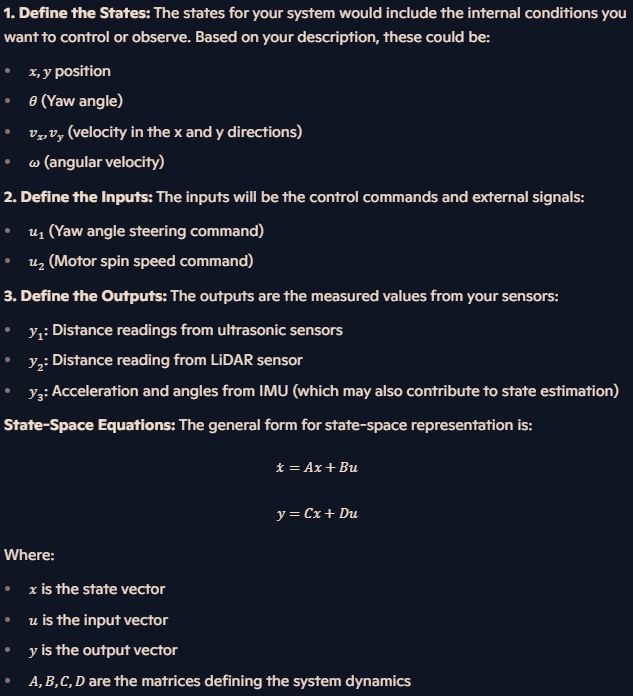
\includegraphics[width=0.535\textwidth]{./Images/copilot-ssr.JPG}
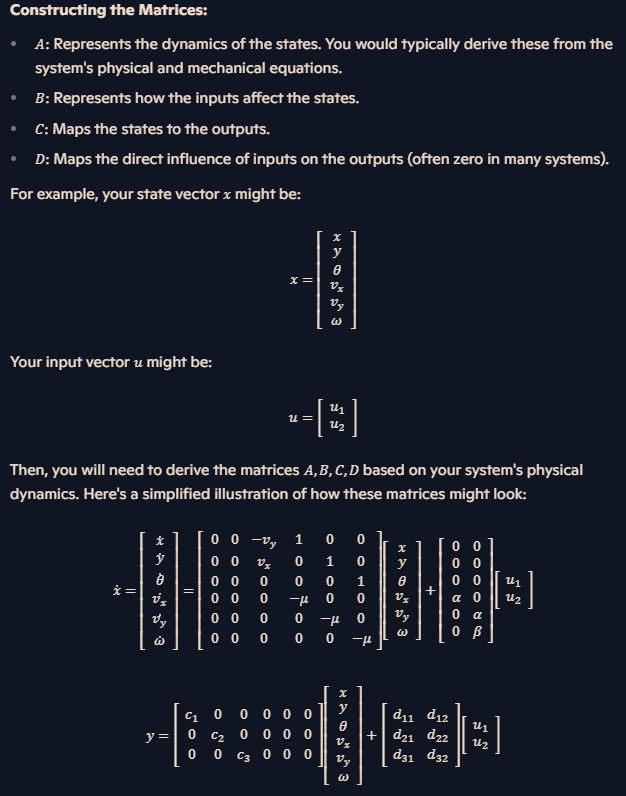
\includegraphics[width=0.465\textwidth]{./Images/copilot-ssr2.JPG}

\underline{\textit{Microsoft Copilot Output \#2: FCC}}\\

\noindent \textbf{Q:} fcc acronym

\noindent \textbf{A:} \\
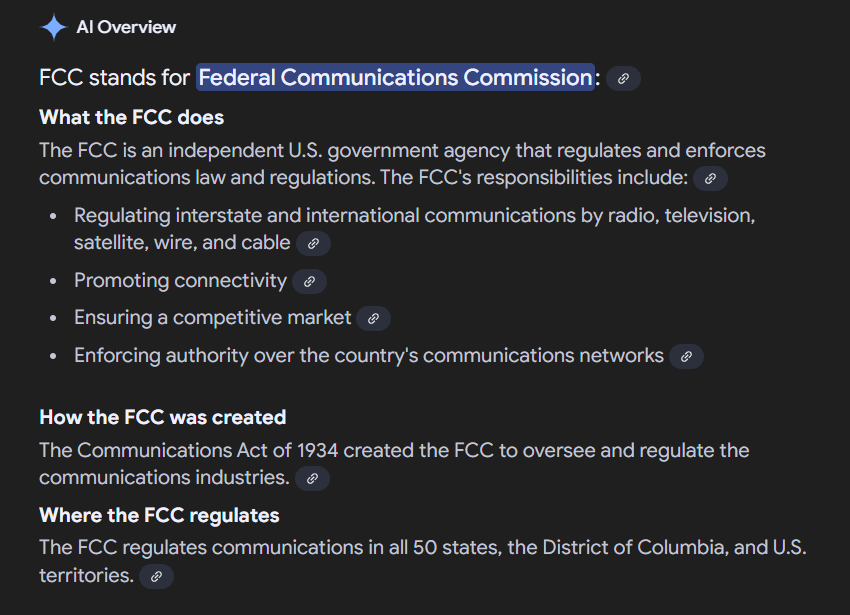
\includegraphics[width=0.535\textwidth]{./Images/fcc_ai.png}

	
	\end{singlespace}
\end{document}

